\documentclass[a4paper]{book}
\usepackage{a4wide}
\usepackage{makeidx}
\usepackage{graphicx}
\usepackage{multicol}
\usepackage{float}
\usepackage{listings}
\usepackage{color}
\usepackage{textcomp}
\usepackage{alltt}
\usepackage{times}
\usepackage{ifpdf}
\ifpdf
\usepackage[pdftex,
            pagebackref=true,
            colorlinks=true,
            linkcolor=blue,
            unicode
           ]{hyperref}
\else
\usepackage[ps2pdf,
            pagebackref=true,
            colorlinks=true,
            linkcolor=blue,
            unicode
           ]{hyperref}
\usepackage{pspicture}
\fi
\usepackage[utf8]{inputenc}
\usepackage{doxygen}
\lstset{language=C++,inputencoding=utf8,basicstyle=\footnotesize,breaklines=true,breakatwhitespace=true,tabsize=8,numbers=left }
\makeindex
\setcounter{tocdepth}{3}
\renewcommand{\footrulewidth}{0.4pt}
\begin{document}
\hypersetup{pageanchor=false}
\begin{titlepage}
\vspace*{7cm}
\begin{center}
{\Large 3D Player }\\
\vspace*{1cm}
{\large Generated by Doxygen 1.6.3}\\
\vspace*{0.5cm}
{\small Thu Jun 10 22:05:23 2010}\\
\end{center}
\end{titlepage}
\clearemptydoublepage
\pagenumbering{roman}
\tableofcontents
\clearemptydoublepage
\pagenumbering{arabic}
\hypersetup{pageanchor=true}
\chapter{Class Index}
\section{Class List}
Here are the classes, structs, unions and interfaces with brief descriptions:\begin{DoxyCompactList}
\item\contentsline{section}{\hyperlink{struct___nv___stereo___image___header}{\_\-Nv\_\-Stereo\_\-Image\_\-Header} }{\pageref{struct___nv___stereo___image___header}}{}
\item\contentsline{section}{\hyperlink{class_my_timer}{MyTimer} }{\pageref{class_my_timer}}{}
\end{DoxyCompactList}

\chapter{File Index}
\section{File List}
Here is a list of all files with brief descriptions:\begin{DoxyCompactList}
\item\contentsline{section}{MVCCommonLib/\hyperlink{_array_list_8h}{ArrayList.h} }{\pageref{_array_list_8h}}{}
\item\contentsline{section}{MVCCommonLib/\hyperlink{_common_8h}{Common.h} }{\pageref{_common_8h}}{}
\item\contentsline{section}{MVCCommonLib/\hyperlink{_debug_8cpp}{Debug.cpp} }{\pageref{_debug_8cpp}}{}
\item\contentsline{section}{MVCCommonLib/\hyperlink{_debug_8h}{Debug.h} }{\pageref{_debug_8h}}{}
\item\contentsline{section}{MVCCommonLib/\hyperlink{_macros_8h}{Macros.h} }{\pageref{_macros_8h}}{}
\item\contentsline{section}{MVCCommonLib/\hyperlink{_pair_8h}{Pair.h} }{\pageref{_pair_8h}}{}
\item\contentsline{section}{MVCCommonLib/\hyperlink{_picture_info_8h}{PictureInfo.h} }{\pageref{_picture_info_8h}}{}
\item\contentsline{section}{MVCCommonLib/\hyperlink{_sliding_window_8cpp}{SlidingWindow.cpp} }{\pageref{_sliding_window_8cpp}}{}
\item\contentsline{section}{MVCCommonLib/\hyperlink{_sliding_window_8h}{SlidingWindow.h} }{\pageref{_sliding_window_8h}}{}
\item\contentsline{section}{MVCCommonLib/\hyperlink{_types_8h}{Types.h} }{\pageref{_types_8h}}{}
\item\contentsline{section}{MVCCommonLib/Arch/\hyperlink{_arch_8h}{Arch.h} }{\pageref{_arch_8h}}{}
\item\contentsline{section}{MVCCommonLib/Arch/Linux/\hyperlink{_arch_linux_8cpp}{ArchLinux.cpp} }{\pageref{_arch_linux_8cpp}}{}
\item\contentsline{section}{MVCCommonLib/Arch/Linux/\hyperlink{_arch_linux_8h}{ArchLinux.h} }{\pageref{_arch_linux_8h}}{}
\item\contentsline{section}{MVCCommonLib/Arch/LinuxCELL/\hyperlink{_arch_c_e_l_l_8cpp}{ArchCELL.cpp} }{\pageref{_arch_c_e_l_l_8cpp}}{}
\item\contentsline{section}{MVCCommonLib/Arch/LinuxCELL/\hyperlink{_arch_c_e_l_l_8h}{ArchCELL.h} }{\pageref{_arch_c_e_l_l_8h}}{}
\item\contentsline{section}{MVCCommonLib/Arch/LinuxCELL/\hyperlink{_arch_p_p_u_8cpp}{ArchPPU.cpp} }{\pageref{_arch_p_p_u_8cpp}}{}
\item\contentsline{section}{MVCCommonLib/Arch/LinuxCELL/\hyperlink{_arch_p_p_u_8h}{ArchPPU.h} }{\pageref{_arch_p_p_u_8h}}{}
\item\contentsline{section}{MVCCommonLib/Arch/LinuxCELL/\hyperlink{_arch_s_p_u_8cpp}{ArchSPU.cpp} }{\pageref{_arch_s_p_u_8cpp}}{}
\item\contentsline{section}{MVCCommonLib/Arch/LinuxCELL/\hyperlink{_arch_s_p_u_8h}{ArchSPU.h} }{\pageref{_arch_s_p_u_8h}}{}
\item\contentsline{section}{MVCCommonLib/Arch/Windows/\hyperlink{_arch_windows_8cpp}{ArchWindows.cpp} }{\pageref{_arch_windows_8cpp}}{}
\item\contentsline{section}{MVCCommonLib/Arch/Windows/\hyperlink{_arch_windows_8h}{ArchWindows.h} }{\pageref{_arch_windows_8h}}{}
\item\contentsline{section}{MVCCommonLib/Codec/\hyperlink{_bitstream_8h}{Bitstream.h} }{\pageref{_bitstream_8h}}{}
\item\contentsline{section}{MVCCommonLib/Codec/\hyperlink{_consts4_standard_8h}{Consts4Standard.h} }{\pageref{_consts4_standard_8h}}{}
\item\contentsline{section}{MVCCommonLib/Codec/\hyperlink{_loop_filter_8cpp}{LoopFilter.cpp} }{\pageref{_loop_filter_8cpp}}{}
\item\contentsline{section}{MVCCommonLib/Codec/\hyperlink{_loop_filter_8h}{LoopFilter.h} }{\pageref{_loop_filter_8h}}{}
\item\contentsline{section}{MVCCommonLib/Codec/\hyperlink{_m_v_c_common_lib_2_codec_2_p_b_predict_8cpp}{PBPredict.cpp} }{\pageref{_m_v_c_common_lib_2_codec_2_p_b_predict_8cpp}}{}
\item\contentsline{section}{MVCCommonLib/Codec/\hyperlink{_m_v_c_common_lib_2_codec_2_p_b_predict_8h}{PBPredict.h} }{\pageref{_m_v_c_common_lib_2_codec_2_p_b_predict_8h}}{}
\item\contentsline{section}{MVCCommonLib/Codec/\hyperlink{_picture_param_8h}{PictureParam.h} }{\pageref{_picture_param_8h}}{}
\item\contentsline{section}{MVCCommonLib/Codec/\hyperlink{_sequence_param_8h}{SequenceParam.h} }{\pageref{_sequence_param_8h}}{}
\item\contentsline{section}{MVCCommonLib/Codec/\hyperlink{_slice_param_8h}{SliceParam.h} }{\pageref{_slice_param_8h}}{}
\item\contentsline{section}{MVCCommonLib/Codec/\hyperlink{vlc_8h}{vlc.h} }{\pageref{vlc_8h}}{}
\item\contentsline{section}{MVCCommonLib/Codec/\hyperlink{vlc_pred_8cpp}{vlcPred.cpp} }{\pageref{vlc_pred_8cpp}}{}
\item\contentsline{section}{MVCCommonLib/Codec/\hyperlink{vlc_pred_8h}{vlcPred.h} }{\pageref{vlc_pred_8h}}{}
\item\contentsline{section}{MVCCommonLib/Codec/IFrame/\hyperlink{_i_predict_8cpp}{IPredict.cpp} }{\pageref{_i_predict_8cpp}}{}
\item\contentsline{section}{MVCCommonLib/Codec/IFrame/\hyperlink{_i_predict_8h}{IPredict.h} }{\pageref{_i_predict_8h}}{}
\item\contentsline{section}{MVCDecoder/\hyperlink{_bitstream_data_8h}{BitstreamData.h} }{\pageref{_bitstream_data_8h}}{}
\item\contentsline{section}{MVCDecoder/\hyperlink{_codec_info_8cpp}{CodecInfo.cpp} }{\pageref{_codec_info_8cpp}}{}
\item\contentsline{section}{MVCDecoder/\hyperlink{_codec_info_8h}{CodecInfo.h} }{\pageref{_codec_info_8h}}{}
\item\contentsline{section}{MVCDecoder/\hyperlink{_configure_8cpp}{Configure.cpp} }{\pageref{_configure_8cpp}}{}
\item\contentsline{section}{MVCDecoder/\hyperlink{_configure_8h}{Configure.h} }{\pageref{_configure_8h}}{}
\item\contentsline{section}{MVCDecoder/\hyperlink{_mvc_decoder_8cpp}{MvcDecoder.cpp} }{\pageref{_mvc_decoder_8cpp}}{}
\item\contentsline{section}{MVCDecoder/\hyperlink{_raw_data_8h}{RawData.h} }{\pageref{_raw_data_8h}}{}
\item\contentsline{section}{MVCDecoder/\hyperlink{_task_dispatcher_8cpp}{TaskDispatcher.cpp} }{\pageref{_task_dispatcher_8cpp}}{}
\item\contentsline{section}{MVCDecoder/\hyperlink{_task_dispatcher_8h}{TaskDispatcher.h} }{\pageref{_task_dispatcher_8h}}{}
\item\contentsline{section}{MVCDecoder/Codec/\hyperlink{_c_a_v_l_c_8cpp}{CAVLC.cpp} }{\pageref{_c_a_v_l_c_8cpp}}{}
\item\contentsline{section}{MVCDecoder/Codec/\hyperlink{_c_a_v_l_c_8h}{CAVLC.h} }{\pageref{_c_a_v_l_c_8h}}{}
\item\contentsline{section}{MVCDecoder/Codec/\hyperlink{_configure_slave_8cpp}{ConfigureSlave.cpp} }{\pageref{_configure_slave_8cpp}}{}
\item\contentsline{section}{MVCDecoder/Codec/\hyperlink{_configure_slave_8h}{ConfigureSlave.h} }{\pageref{_configure_slave_8h}}{}
\item\contentsline{section}{MVCDecoder/Codec/\hyperlink{_d_c_t_transform_8cpp}{DCTTransform.cpp} }{\pageref{_d_c_t_transform_8cpp}}{}
\item\contentsline{section}{MVCDecoder/Codec/\hyperlink{_d_c_t_transform_8h}{DCTTransform.h} }{\pageref{_d_c_t_transform_8h}}{}
\item\contentsline{section}{MVCDecoder/Codec/\hyperlink{_quantisation_8cpp}{Quantisation.cpp} }{\pageref{_quantisation_8cpp}}{}
\item\contentsline{section}{MVCDecoder/Codec/\hyperlink{_quantisation_8h}{Quantisation.h} }{\pageref{_quantisation_8h}}{}
\item\contentsline{section}{MVCDecoder/Codec/\hyperlink{_scanner_8h}{Scanner.h} }{\pageref{_scanner_8h}}{}
\item\contentsline{section}{MVCDecoder/Codec/IFrame/\hyperlink{_i_c_a_v_l_c_8cpp}{ICAVLC.cpp} }{\pageref{_i_c_a_v_l_c_8cpp}}{}
\item\contentsline{section}{MVCDecoder/Codec/IFrame/\hyperlink{_i_c_a_v_l_c_8h}{ICAVLC.h} }{\pageref{_i_c_a_v_l_c_8h}}{}
\item\contentsline{section}{MVCDecoder/Codec/IFrame/\hyperlink{_i_macroblock_codec_8cpp}{IMacroblockCodec.cpp} }{\pageref{_i_macroblock_codec_8cpp}}{}
\item\contentsline{section}{MVCDecoder/Codec/IFrame/\hyperlink{_i_macroblock_codec_8h}{IMacroblockCodec.h} }{\pageref{_i_macroblock_codec_8h}}{}
\item\contentsline{section}{MVCDecoder/Codec/IFrame/\hyperlink{_i_slice_8cpp}{ISlice.cpp} }{\pageref{_i_slice_8cpp}}{}
\item\contentsline{section}{MVCDecoder/Codec/IFrame/\hyperlink{_i_slice_8h}{ISlice.h} }{\pageref{_i_slice_8h}}{}
\item\contentsline{section}{MVCDecoder/Codec/PBFrame/\hyperlink{_p_b_c_a_v_l_c_8cpp}{PBCAVLC.cpp} }{\pageref{_p_b_c_a_v_l_c_8cpp}}{}
\item\contentsline{section}{MVCDecoder/Codec/PBFrame/\hyperlink{_p_b_c_a_v_l_c_8h}{PBCAVLC.h} }{\pageref{_p_b_c_a_v_l_c_8h}}{}
\item\contentsline{section}{MVCDecoder/Codec/PBFrame/\hyperlink{_p_b_macroblock_codec_8cpp}{PBMacroblockCodec.cpp} }{\pageref{_p_b_macroblock_codec_8cpp}}{}
\item\contentsline{section}{MVCDecoder/Codec/PBFrame/\hyperlink{_p_b_macroblock_codec_8h}{PBMacroblockCodec.h} }{\pageref{_p_b_macroblock_codec_8h}}{}
\item\contentsline{section}{MVCDecoder/Codec/PBFrame/\hyperlink{_m_v_c_decoder_2_codec_2_p_b_frame_2_p_b_predict_8cpp}{PBPredict.cpp} }{\pageref{_m_v_c_decoder_2_codec_2_p_b_frame_2_p_b_predict_8cpp}}{}
\item\contentsline{section}{MVCDecoder/Codec/PBFrame/\hyperlink{_m_v_c_decoder_2_codec_2_p_b_frame_2_p_b_predict_8h}{PBPredict.h} }{\pageref{_m_v_c_decoder_2_codec_2_p_b_frame_2_p_b_predict_8h}}{}
\item\contentsline{section}{MVCDecoder/Codec/PBFrame/\hyperlink{_p_slice_8cpp}{PSlice.cpp} }{\pageref{_p_slice_8cpp}}{}
\item\contentsline{section}{MVCDecoder/Codec/PBFrame/\hyperlink{_p_slice_8h}{PSlice.h} }{\pageref{_p_slice_8h}}{}
\item\contentsline{section}{MVCDecoder/Controller/\hyperlink{_a_frame_controller_8h}{AFrameController.h} }{\pageref{_a_frame_controller_8h}}{}
\item\contentsline{section}{MVCDecoder/Controller/\hyperlink{_frame_controller___parallel_8cpp}{FrameController\_\-Parallel.cpp} }{\pageref{_frame_controller___parallel_8cpp}}{}
\item\contentsline{section}{MVCDecoder/Controller/\hyperlink{_frame_controller___parallel_8h}{FrameController\_\-Parallel.h} }{\pageref{_frame_controller___parallel_8h}}{}
\item\contentsline{section}{MVCDecoder/spu/decodeframe\_\-b/\hyperlink{decodeframe__b_8cpp}{decodeframe\_\-b.cpp} }{\pageref{decodeframe__b_8cpp}}{}
\item\contentsline{section}{MVCDecoder/spu/decodeframe\_\-b/\hyperlink{decodeframe__b_8h}{decodeframe\_\-b.h} }{\pageref{decodeframe__b_8h}}{}
\item\contentsline{section}{MVCDecoder/spu/decodeframe\_\-i/\hyperlink{decodeframe__i_8cpp}{decodeframe\_\-i.cpp} }{\pageref{decodeframe__i_8cpp}}{}
\item\contentsline{section}{MVCDecoder/spu/decodeframe\_\-i/\hyperlink{decodeframe__i_8h}{decodeframe\_\-i.h} }{\pageref{decodeframe__i_8h}}{}
\item\contentsline{section}{MVCDecoder/spu/decodeframe\_\-p/\hyperlink{decodeframe__p_8cpp}{decodeframe\_\-p.cpp} }{\pageref{decodeframe__p_8cpp}}{}
\item\contentsline{section}{MVCDecoder/spu/decodeframe\_\-p/\hyperlink{decodeframe__p_8h}{decodeframe\_\-p.h} }{\pageref{decodeframe__p_8h}}{}
\item\contentsline{section}{MVCDecoder/Stream/\hyperlink{_in_stream_8cpp}{InStream.cpp} }{\pageref{_in_stream_8cpp}}{}
\item\contentsline{section}{MVCDecoder/Stream/\hyperlink{_in_stream_8h}{InStream.h} }{\pageref{_in_stream_8h}}{}
\end{DoxyCompactList}

\chapter{Class Documentation}
\hypertarget{struct___nv___stereo___image___header}{
\section{\_\-Nv\_\-Stereo\_\-Image\_\-Header Struct Reference}
\label{struct___nv___stereo___image___header}\index{\_\-Nv\_\-Stereo\_\-Image\_\-Header@{\_\-Nv\_\-Stereo\_\-Image\_\-Header}}
}


{\ttfamily \#include $<$utils.h$>$}

\subsection*{Public Attributes}
\begin{DoxyCompactItemize}
\item 
unsigned int \hyperlink{struct___nv___stereo___image___header_aac21b6be816ef3e6b98d1f1183263fd9}{dwSignature}
\item 
unsigned int \hyperlink{struct___nv___stereo___image___header_a495218c0378e538de8c3504daa0a0846}{dwWidth}
\item 
unsigned int \hyperlink{struct___nv___stereo___image___header_a72c1451aca7cb9c87540b647d51b25ad}{dwHeight}
\item 
unsigned int \hyperlink{struct___nv___stereo___image___header_a9a51ead5061c21601c50b0e1ee2be9a0}{dwBPP}
\item 
unsigned int \hyperlink{struct___nv___stereo___image___header_ad99da98f0c7e667408c3bba51ff5d047}{dwFlags}
\end{DoxyCompactItemize}


\subsection{Detailed Description}


Definition at line \hyperlink{utils_8h_source_l00007}{7} of file \hyperlink{utils_8h_source}{utils.h}.



\subsection{Member Data Documentation}
\hypertarget{struct___nv___stereo___image___header_a9a51ead5061c21601c50b0e1ee2be9a0}{
\index{\_\-Nv\_\-Stereo\_\-Image\_\-Header@{\_\-Nv\_\-Stereo\_\-Image\_\-Header}!dwBPP@{dwBPP}}
\index{dwBPP@{dwBPP}!_Nv_Stereo_Image_Header@{\_\-Nv\_\-Stereo\_\-Image\_\-Header}}
\subsubsection[{dwBPP}]{\setlength{\rightskip}{0pt plus 5cm}unsigned int {\bf \_\-Nv\_\-Stereo\_\-Image\_\-Header::dwBPP}}}
\label{struct___nv___stereo___image___header_a9a51ead5061c21601c50b0e1ee2be9a0}


Definition at line \hyperlink{utils_8h_source_l00011}{11} of file \hyperlink{utils_8h_source}{utils.h}.

\hypertarget{struct___nv___stereo___image___header_ad99da98f0c7e667408c3bba51ff5d047}{
\index{\_\-Nv\_\-Stereo\_\-Image\_\-Header@{\_\-Nv\_\-Stereo\_\-Image\_\-Header}!dwFlags@{dwFlags}}
\index{dwFlags@{dwFlags}!_Nv_Stereo_Image_Header@{\_\-Nv\_\-Stereo\_\-Image\_\-Header}}
\subsubsection[{dwFlags}]{\setlength{\rightskip}{0pt plus 5cm}unsigned int {\bf \_\-Nv\_\-Stereo\_\-Image\_\-Header::dwFlags}}}
\label{struct___nv___stereo___image___header_ad99da98f0c7e667408c3bba51ff5d047}


Definition at line \hyperlink{utils_8h_source_l00012}{12} of file \hyperlink{utils_8h_source}{utils.h}.

\hypertarget{struct___nv___stereo___image___header_a72c1451aca7cb9c87540b647d51b25ad}{
\index{\_\-Nv\_\-Stereo\_\-Image\_\-Header@{\_\-Nv\_\-Stereo\_\-Image\_\-Header}!dwHeight@{dwHeight}}
\index{dwHeight@{dwHeight}!_Nv_Stereo_Image_Header@{\_\-Nv\_\-Stereo\_\-Image\_\-Header}}
\subsubsection[{dwHeight}]{\setlength{\rightskip}{0pt plus 5cm}unsigned int {\bf \_\-Nv\_\-Stereo\_\-Image\_\-Header::dwHeight}}}
\label{struct___nv___stereo___image___header_a72c1451aca7cb9c87540b647d51b25ad}


Definition at line \hyperlink{utils_8h_source_l00010}{10} of file \hyperlink{utils_8h_source}{utils.h}.

\hypertarget{struct___nv___stereo___image___header_aac21b6be816ef3e6b98d1f1183263fd9}{
\index{\_\-Nv\_\-Stereo\_\-Image\_\-Header@{\_\-Nv\_\-Stereo\_\-Image\_\-Header}!dwSignature@{dwSignature}}
\index{dwSignature@{dwSignature}!_Nv_Stereo_Image_Header@{\_\-Nv\_\-Stereo\_\-Image\_\-Header}}
\subsubsection[{dwSignature}]{\setlength{\rightskip}{0pt plus 5cm}unsigned int {\bf \_\-Nv\_\-Stereo\_\-Image\_\-Header::dwSignature}}}
\label{struct___nv___stereo___image___header_aac21b6be816ef3e6b98d1f1183263fd9}


Definition at line \hyperlink{utils_8h_source_l00008}{8} of file \hyperlink{utils_8h_source}{utils.h}.

\hypertarget{struct___nv___stereo___image___header_a495218c0378e538de8c3504daa0a0846}{
\index{\_\-Nv\_\-Stereo\_\-Image\_\-Header@{\_\-Nv\_\-Stereo\_\-Image\_\-Header}!dwWidth@{dwWidth}}
\index{dwWidth@{dwWidth}!_Nv_Stereo_Image_Header@{\_\-Nv\_\-Stereo\_\-Image\_\-Header}}
\subsubsection[{dwWidth}]{\setlength{\rightskip}{0pt plus 5cm}unsigned int {\bf \_\-Nv\_\-Stereo\_\-Image\_\-Header::dwWidth}}}
\label{struct___nv___stereo___image___header_a495218c0378e538de8c3504daa0a0846}


Definition at line \hyperlink{utils_8h_source_l00009}{9} of file \hyperlink{utils_8h_source}{utils.h}.



The documentation for this struct was generated from the following file:\begin{DoxyCompactItemize}
\item 
/Volumes/BOOTCAMP/Workspace/Solutions/MVC/proj/Direct3DTutorial/Direct3DTutorial/\hyperlink{utils_8h}{utils.h}\end{DoxyCompactItemize}

\hypertarget{class_my_timer}{
\section{MyTimer Class Reference}
\label{class_my_timer}\index{MyTimer@{MyTimer}}
}


{\ttfamily \#include $<$mytimer.h$>$}

\subsection*{Public Member Functions}
\begin{DoxyCompactItemize}
\item 
\hyperlink{class_my_timer_a75440365bcfd96d34be38d8a0c9c014b}{MyTimer} ()
\item 
void \hyperlink{class_my_timer_a74b18b409d493579f6b3d0972590a7a6}{Start} ()
\item 
void \hyperlink{class_my_timer_a9c499fe726dbd8a30c528727f42e993d}{End} ()
\item 
LONGLONG \hyperlink{class_my_timer_abd0f6728cf64f7b5d81235588bb8e3c2}{getElapsedTime} ()
\item 
void \hyperlink{class_my_timer_ae616c920850e8d388f93f0d354b25ba5}{Reset} ()
\item 
unsigned \_\-\_\-int64 \hyperlink{class_my_timer_ae695b0dd5d9c28c1d3dc46ba4c616eec}{GetCycleCount} ()
\end{DoxyCompactItemize}
\subsection*{Public Attributes}
\begin{DoxyCompactItemize}
\item 
LONGLONG \hyperlink{class_my_timer_adef1d73f6cbdc533c45766b6fa739154}{costTime}
\end{DoxyCompactItemize}


\subsection{Detailed Description}


Definition at line \hyperlink{mytimer_8h_source_l00005}{5} of file \hyperlink{mytimer_8h_source}{mytimer.h}.



\subsection{Constructor \& Destructor Documentation}
\hypertarget{class_my_timer_a75440365bcfd96d34be38d8a0c9c014b}{
\index{MyTimer@{MyTimer}!MyTimer@{MyTimer}}
\index{MyTimer@{MyTimer}!MyTimer@{MyTimer}}
\subsubsection[{MyTimer}]{\setlength{\rightskip}{0pt plus 5cm}MyTimer::MyTimer ()\hspace{0.3cm}{\ttfamily  \mbox{[}inline\mbox{]}}}}
\label{class_my_timer_a75440365bcfd96d34be38d8a0c9c014b}


Definition at line \hyperlink{mytimer_8h_source_l00016}{16} of file \hyperlink{mytimer_8h_source}{mytimer.h}.



\subsection{Member Function Documentation}
\hypertarget{class_my_timer_a9c499fe726dbd8a30c528727f42e993d}{
\index{MyTimer@{MyTimer}!End@{End}}
\index{End@{End}!MyTimer@{MyTimer}}
\subsubsection[{End}]{\setlength{\rightskip}{0pt plus 5cm}void MyTimer::End ()\hspace{0.3cm}{\ttfamily  \mbox{[}inline\mbox{]}}}}
\label{class_my_timer_a9c499fe726dbd8a30c528727f42e993d}


Definition at line \hyperlink{mytimer_8h_source_l00027}{27} of file \hyperlink{mytimer_8h_source}{mytimer.h}.

\hypertarget{class_my_timer_ae695b0dd5d9c28c1d3dc46ba4c616eec}{
\index{MyTimer@{MyTimer}!GetCycleCount@{GetCycleCount}}
\index{GetCycleCount@{GetCycleCount}!MyTimer@{MyTimer}}
\subsubsection[{GetCycleCount}]{\setlength{\rightskip}{0pt plus 5cm}unsigned \_\-\_\-int64 MyTimer::GetCycleCount ()\hspace{0.3cm}{\ttfamily  \mbox{[}inline\mbox{]}}}}
\label{class_my_timer_ae695b0dd5d9c28c1d3dc46ba4c616eec}


Definition at line \hyperlink{mytimer_8h_source_l00041}{41} of file \hyperlink{mytimer_8h_source}{mytimer.h}.

\hypertarget{class_my_timer_abd0f6728cf64f7b5d81235588bb8e3c2}{
\index{MyTimer@{MyTimer}!getElapsedTime@{getElapsedTime}}
\index{getElapsedTime@{getElapsedTime}!MyTimer@{MyTimer}}
\subsubsection[{getElapsedTime}]{\setlength{\rightskip}{0pt plus 5cm}LONGLONG MyTimer::getElapsedTime ()\hspace{0.3cm}{\ttfamily  \mbox{[}inline\mbox{]}}}}
\label{class_my_timer_abd0f6728cf64f7b5d81235588bb8e3c2}


Definition at line \hyperlink{mytimer_8h_source_l00032}{32} of file \hyperlink{mytimer_8h_source}{mytimer.h}.



Here is the caller graph for this function:\nopagebreak
\begin{figure}[H]
\begin{center}
\leavevmode
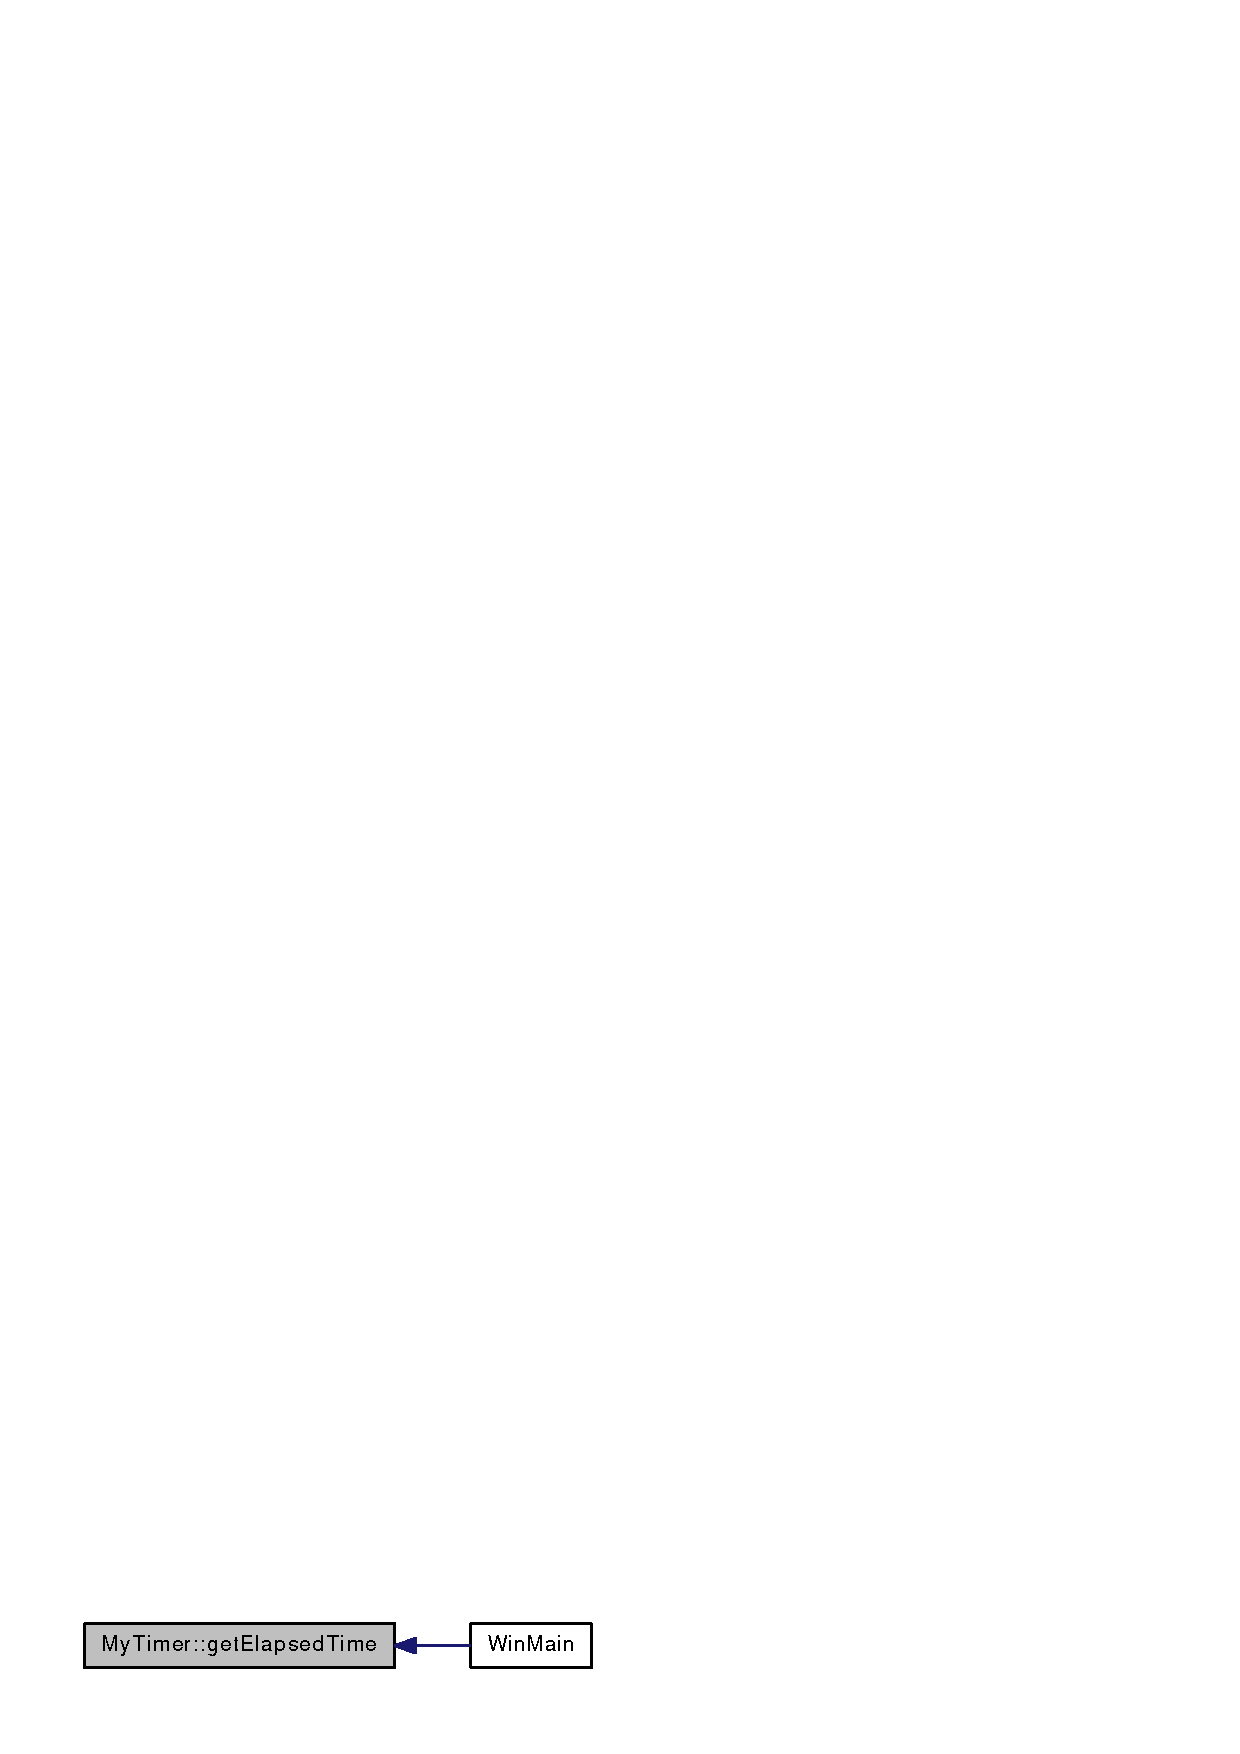
\includegraphics[width=144pt]{class_my_timer_abd0f6728cf64f7b5d81235588bb8e3c2_icgraph}
\end{center}
\end{figure}


\hypertarget{class_my_timer_ae616c920850e8d388f93f0d354b25ba5}{
\index{MyTimer@{MyTimer}!Reset@{Reset}}
\index{Reset@{Reset}!MyTimer@{MyTimer}}
\subsubsection[{Reset}]{\setlength{\rightskip}{0pt plus 5cm}void MyTimer::Reset ()\hspace{0.3cm}{\ttfamily  \mbox{[}inline\mbox{]}}}}
\label{class_my_timer_ae616c920850e8d388f93f0d354b25ba5}


Definition at line \hyperlink{mytimer_8h_source_l00037}{37} of file \hyperlink{mytimer_8h_source}{mytimer.h}.

\hypertarget{class_my_timer_a74b18b409d493579f6b3d0972590a7a6}{
\index{MyTimer@{MyTimer}!Start@{Start}}
\index{Start@{Start}!MyTimer@{MyTimer}}
\subsubsection[{Start}]{\setlength{\rightskip}{0pt plus 5cm}void MyTimer::Start ()\hspace{0.3cm}{\ttfamily  \mbox{[}inline\mbox{]}}}}
\label{class_my_timer_a74b18b409d493579f6b3d0972590a7a6}


Definition at line \hyperlink{mytimer_8h_source_l00023}{23} of file \hyperlink{mytimer_8h_source}{mytimer.h}.



Here is the caller graph for this function:\nopagebreak
\begin{figure}[H]
\begin{center}
\leavevmode
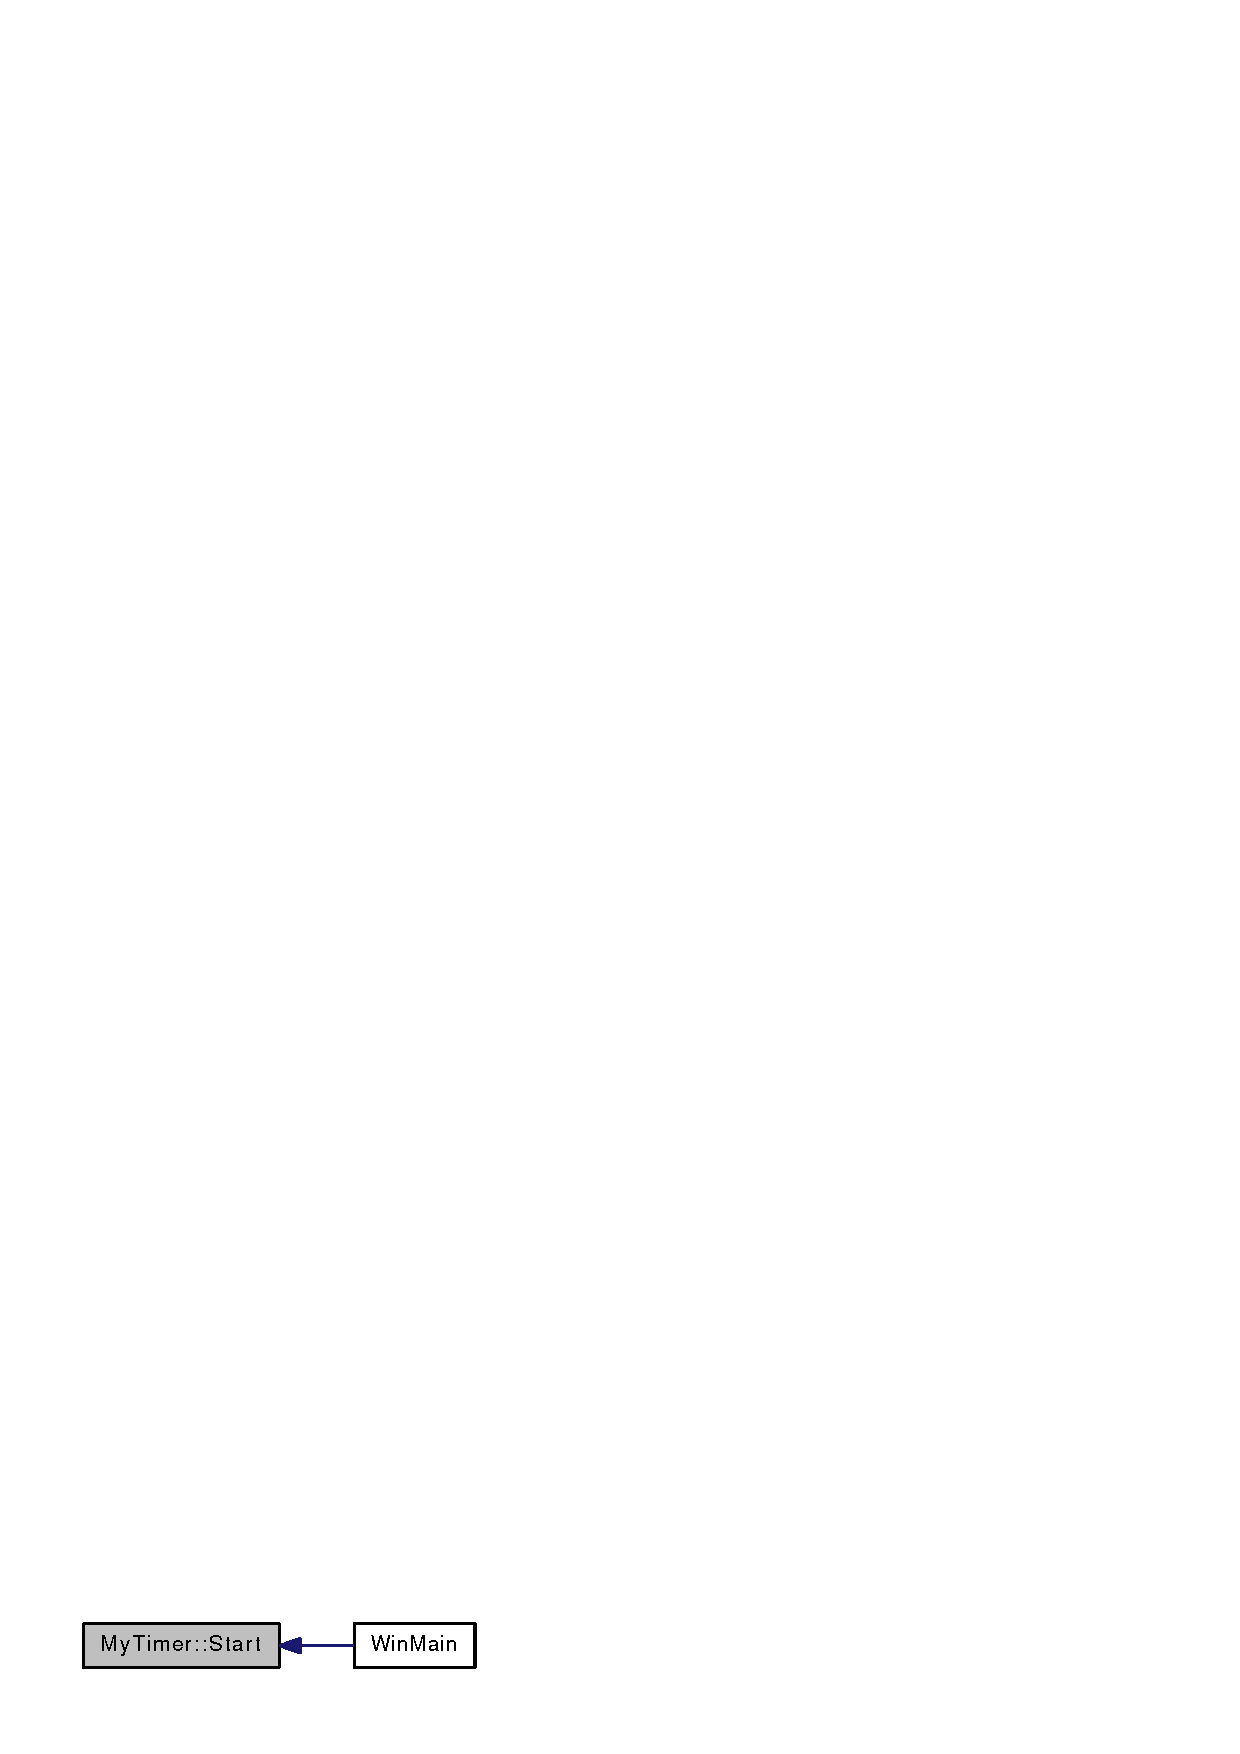
\includegraphics[width=116pt]{class_my_timer_a74b18b409d493579f6b3d0972590a7a6_icgraph}
\end{center}
\end{figure}




\subsection{Member Data Documentation}
\hypertarget{class_my_timer_adef1d73f6cbdc533c45766b6fa739154}{
\index{MyTimer@{MyTimer}!costTime@{costTime}}
\index{costTime@{costTime}!MyTimer@{MyTimer}}
\subsubsection[{costTime}]{\setlength{\rightskip}{0pt plus 5cm}LONGLONG {\bf MyTimer::costTime}}}
\label{class_my_timer_adef1d73f6cbdc533c45766b6fa739154}


Definition at line \hyperlink{mytimer_8h_source_l00013}{13} of file \hyperlink{mytimer_8h_source}{mytimer.h}.



The documentation for this class was generated from the following file:\begin{DoxyCompactItemize}
\item 
/Volumes/BOOTCAMP/Workspace/Solutions/MVC/proj/Direct3DTutorial/Direct3DTutorial/\hyperlink{mytimer_8h}{mytimer.h}\end{DoxyCompactItemize}

\chapter{File Documentation}
\hypertarget{config_8h}{
\section{/Volumes/BOOTCAMP/Workspace/Solutions/MVC/proj/Direct3DTutorial/Direct3DTutorial/config.h File Reference}
\label{config_8h}\index{/Volumes/BOOTCAMP/Workspace/Solutions/MVC/proj/Direct3DTutorial/Direct3DTutorial/config.h@{/Volumes/BOOTCAMP/Workspace/Solutions/MVC/proj/Direct3DTutorial/Direct3DTutorial/config.h}}
}
\subsection*{Variables}
\begin{DoxyCompactItemize}
\item 
int \hyperlink{config_8h_a5dde88e08c88df4ec4c201ab068a909b}{gImageWidth} = 720
\item 
int \hyperlink{config_8h_af737c15e6577f2676602957bc1ac2ab1}{gImageHeight} = 576
\item 
wstring \hyperlink{config_8h_a526270325c61739d50933ee42ef9563f}{filenameWstrL}
\item 
wstring \hyperlink{config_8h_a3b06e388f8261198f0fe86aafca02c41}{filenameWstrR}
\item 
string \hyperlink{config_8h_a65980faa7a98d89e3581eb3ac8777192}{filenameStrL}
\item 
string \hyperlink{config_8h_a19fa526345d6a5020afd0ef78ab58f71}{filenameStrR}
\item 
LPCWSTR \hyperlink{config_8h_a9e78e5f975acc8e56d6a84214321a534}{filenameL}
\item 
LPCWSTR \hyperlink{config_8h_ab2d091b589f33f799378b4dbf379e537}{filenameR}
\item 
LPCSTR \hyperlink{config_8h_a4efd8a98fc24b184ad75501454b3c2b7}{filenameLL}
\item 
LPCSTR \hyperlink{config_8h_ac31be6060769b3c9c0c533e0cf269b28}{filenameRR}
\item 
string \hyperlink{config_8h_a5cfb7ac53a84ac65db638d7926c1216b}{prefixL1} = \char`\"{}../imgSeq/Knights\_\-Quest/L/Knights\_\-Quest\_\-576p\char`\"{}
\item 
string \hyperlink{config_8h_a0cc8c7e0d207c825f13d92d52480abfc}{prefixR1} = \char`\"{}../imgSeq/Knights\_\-Quest/R/Knights\_\-Quest\_\-576p\char`\"{}
\item 
string \hyperlink{config_8h_a887452eecbb8843e5530a1597eb8e357}{suffix} = \char`\"{}.jpg\char`\"{}
\item 
int \hyperlink{config_8h_a1daaec6dd86a744de60951adc0d7491c}{totalFrames1} = 2615
\item 
string \hyperlink{config_8h_ad2536ccefd202465bc9de3185f689385}{prefixL2} = \char`\"{}../imgSeq/twoeye/L/twoeye\_\-720x576\char`\"{}
\item 
string \hyperlink{config_8h_a655684630849cbc78a1a701627a5be79}{prefixR2} = \char`\"{}../imgSeq/twoeye/R/twoeye\_\-720x576\char`\"{}
\item 
int \hyperlink{config_8h_a30f8e88254cae72861ca9f1082036f13}{totalFrames2} = 1608
\item 
string \hyperlink{config_8h_afcc1487cc6eb36a2fc6233b441f2787b}{prefixL3} = \char`\"{}../imgSeq/Demo/L/Demo\_\-\char`\"{}
\item 
string \hyperlink{config_8h_ad994e29c70b4b20e5aa11c462d2eaa23}{prefixR3} = \char`\"{}../imgSeq/Demo/R/Demo\_\-\char`\"{}
\item 
int \hyperlink{config_8h_a4058af0c43622045689a17dbf546a095}{totalFrames3} = 539
\item 
int \hyperlink{config_8h_a64af52e30206638c00ad08ee8894e3c8}{demo} = 2
\item 
string \hyperlink{config_8h_a6082de4d3555d07a84270f7bacac9a63}{prefixL} = \hyperlink{config_8h_ad2536ccefd202465bc9de3185f689385}{prefixL2}
\item 
string \hyperlink{config_8h_a939852ed72b1f29dd46c267ba1894687}{prefixR} = \hyperlink{config_8h_a655684630849cbc78a1a701627a5be79}{prefixR2}
\item 
int \hyperlink{config_8h_a0186bee82f4d469206cfcb18da843a46}{totalFrames} = \hyperlink{config_8h_a30f8e88254cae72861ca9f1082036f13}{totalFrames2}
\item 
double \hyperlink{config_8h_a63da2a617b72a1630998a4d8b4d26cd3}{fps} = 25
\item 
ofstream \hyperlink{config_8h_a0a2814a2252fee90794304506ef2e9c0}{fout}
\end{DoxyCompactItemize}


\subsection{Variable Documentation}
\hypertarget{config_8h_a64af52e30206638c00ad08ee8894e3c8}{
\index{config.h@{config.h}!demo@{demo}}
\index{demo@{demo}!config.h@{config.h}}
\subsubsection[{demo}]{\setlength{\rightskip}{0pt plus 5cm}int {\bf demo} = 2}}
\label{config_8h_a64af52e30206638c00ad08ee8894e3c8}


Definition at line \hyperlink{config_8h_source_l00032}{32} of file \hyperlink{config_8h_source}{config.h}.

\hypertarget{config_8h_a9e78e5f975acc8e56d6a84214321a534}{
\index{config.h@{config.h}!filenameL@{filenameL}}
\index{filenameL@{filenameL}!config.h@{config.h}}
\subsubsection[{filenameL}]{\setlength{\rightskip}{0pt plus 5cm}LPCWSTR {\bf filenameL}}}
\label{config_8h_a9e78e5f975acc8e56d6a84214321a534}


Definition at line \hyperlink{config_8h_source_l00011}{11} of file \hyperlink{config_8h_source}{config.h}.

\hypertarget{config_8h_a4efd8a98fc24b184ad75501454b3c2b7}{
\index{config.h@{config.h}!filenameLL@{filenameLL}}
\index{filenameLL@{filenameLL}!config.h@{config.h}}
\subsubsection[{filenameLL}]{\setlength{\rightskip}{0pt plus 5cm}LPCSTR {\bf filenameLL}}}
\label{config_8h_a4efd8a98fc24b184ad75501454b3c2b7}


Definition at line \hyperlink{config_8h_source_l00012}{12} of file \hyperlink{config_8h_source}{config.h}.

\hypertarget{config_8h_ab2d091b589f33f799378b4dbf379e537}{
\index{config.h@{config.h}!filenameR@{filenameR}}
\index{filenameR@{filenameR}!config.h@{config.h}}
\subsubsection[{filenameR}]{\setlength{\rightskip}{0pt plus 5cm}LPCWSTR {\bf filenameR}}}
\label{config_8h_ab2d091b589f33f799378b4dbf379e537}


Definition at line \hyperlink{config_8h_source_l00011}{11} of file \hyperlink{config_8h_source}{config.h}.

\hypertarget{config_8h_ac31be6060769b3c9c0c533e0cf269b28}{
\index{config.h@{config.h}!filenameRR@{filenameRR}}
\index{filenameRR@{filenameRR}!config.h@{config.h}}
\subsubsection[{filenameRR}]{\setlength{\rightskip}{0pt plus 5cm}LPCSTR {\bf filenameRR}}}
\label{config_8h_ac31be6060769b3c9c0c533e0cf269b28}


Definition at line \hyperlink{config_8h_source_l00012}{12} of file \hyperlink{config_8h_source}{config.h}.

\hypertarget{config_8h_a65980faa7a98d89e3581eb3ac8777192}{
\index{config.h@{config.h}!filenameStrL@{filenameStrL}}
\index{filenameStrL@{filenameStrL}!config.h@{config.h}}
\subsubsection[{filenameStrL}]{\setlength{\rightskip}{0pt plus 5cm}string {\bf filenameStrL}}}
\label{config_8h_a65980faa7a98d89e3581eb3ac8777192}


Definition at line \hyperlink{config_8h_source_l00010}{10} of file \hyperlink{config_8h_source}{config.h}.

\hypertarget{config_8h_a19fa526345d6a5020afd0ef78ab58f71}{
\index{config.h@{config.h}!filenameStrR@{filenameStrR}}
\index{filenameStrR@{filenameStrR}!config.h@{config.h}}
\subsubsection[{filenameStrR}]{\setlength{\rightskip}{0pt plus 5cm}string {\bf filenameStrR}}}
\label{config_8h_a19fa526345d6a5020afd0ef78ab58f71}


Definition at line \hyperlink{config_8h_source_l00010}{10} of file \hyperlink{config_8h_source}{config.h}.

\hypertarget{config_8h_a526270325c61739d50933ee42ef9563f}{
\index{config.h@{config.h}!filenameWstrL@{filenameWstrL}}
\index{filenameWstrL@{filenameWstrL}!config.h@{config.h}}
\subsubsection[{filenameWstrL}]{\setlength{\rightskip}{0pt plus 5cm}wstring {\bf filenameWstrL}}}
\label{config_8h_a526270325c61739d50933ee42ef9563f}


Definition at line \hyperlink{config_8h_source_l00009}{9} of file \hyperlink{config_8h_source}{config.h}.

\hypertarget{config_8h_a3b06e388f8261198f0fe86aafca02c41}{
\index{config.h@{config.h}!filenameWstrR@{filenameWstrR}}
\index{filenameWstrR@{filenameWstrR}!config.h@{config.h}}
\subsubsection[{filenameWstrR}]{\setlength{\rightskip}{0pt plus 5cm}wstring {\bf filenameWstrR}}}
\label{config_8h_a3b06e388f8261198f0fe86aafca02c41}


Definition at line \hyperlink{config_8h_source_l00009}{9} of file \hyperlink{config_8h_source}{config.h}.

\hypertarget{config_8h_a0a2814a2252fee90794304506ef2e9c0}{
\index{config.h@{config.h}!fout@{fout}}
\index{fout@{fout}!config.h@{config.h}}
\subsubsection[{fout}]{\setlength{\rightskip}{0pt plus 5cm}ofstream {\bf fout}}}
\label{config_8h_a0a2814a2252fee90794304506ef2e9c0}


Definition at line \hyperlink{config_8h_source_l00046}{46} of file \hyperlink{config_8h_source}{config.h}.

\hypertarget{config_8h_a63da2a617b72a1630998a4d8b4d26cd3}{
\index{config.h@{config.h}!fps@{fps}}
\index{fps@{fps}!config.h@{config.h}}
\subsubsection[{fps}]{\setlength{\rightskip}{0pt plus 5cm}double {\bf fps} = 25}}
\label{config_8h_a63da2a617b72a1630998a4d8b4d26cd3}


Definition at line \hyperlink{config_8h_source_l00043}{43} of file \hyperlink{config_8h_source}{config.h}.

\hypertarget{config_8h_af737c15e6577f2676602957bc1ac2ab1}{
\index{config.h@{config.h}!gImageHeight@{gImageHeight}}
\index{gImageHeight@{gImageHeight}!config.h@{config.h}}
\subsubsection[{gImageHeight}]{\setlength{\rightskip}{0pt plus 5cm}int {\bf gImageHeight} = 576}}
\label{config_8h_af737c15e6577f2676602957bc1ac2ab1}


Definition at line \hyperlink{config_8h_source_l00008}{8} of file \hyperlink{config_8h_source}{config.h}.

\hypertarget{config_8h_a5dde88e08c88df4ec4c201ab068a909b}{
\index{config.h@{config.h}!gImageWidth@{gImageWidth}}
\index{gImageWidth@{gImageWidth}!config.h@{config.h}}
\subsubsection[{gImageWidth}]{\setlength{\rightskip}{0pt plus 5cm}int {\bf gImageWidth} = 720}}
\label{config_8h_a5dde88e08c88df4ec4c201ab068a909b}


Definition at line \hyperlink{config_8h_source_l00007}{7} of file \hyperlink{config_8h_source}{config.h}.

\hypertarget{config_8h_a6082de4d3555d07a84270f7bacac9a63}{
\index{config.h@{config.h}!prefixL@{prefixL}}
\index{prefixL@{prefixL}!config.h@{config.h}}
\subsubsection[{prefixL}]{\setlength{\rightskip}{0pt plus 5cm}string {\bf prefixL} = {\bf prefixL2}}}
\label{config_8h_a6082de4d3555d07a84270f7bacac9a63}


Definition at line \hyperlink{config_8h_source_l00033}{33} of file \hyperlink{config_8h_source}{config.h}.

\hypertarget{config_8h_a5cfb7ac53a84ac65db638d7926c1216b}{
\index{config.h@{config.h}!prefixL1@{prefixL1}}
\index{prefixL1@{prefixL1}!config.h@{config.h}}
\subsubsection[{prefixL1}]{\setlength{\rightskip}{0pt plus 5cm}string {\bf prefixL1} = \char`\"{}../imgSeq/Knights\_\-Quest/L/Knights\_\-Quest\_\-576p\char`\"{}}}
\label{config_8h_a5cfb7ac53a84ac65db638d7926c1216b}


Definition at line \hyperlink{config_8h_source_l00015}{15} of file \hyperlink{config_8h_source}{config.h}.

\hypertarget{config_8h_ad2536ccefd202465bc9de3185f689385}{
\index{config.h@{config.h}!prefixL2@{prefixL2}}
\index{prefixL2@{prefixL2}!config.h@{config.h}}
\subsubsection[{prefixL2}]{\setlength{\rightskip}{0pt plus 5cm}string {\bf prefixL2} = \char`\"{}../imgSeq/twoeye/L/twoeye\_\-720x576\char`\"{}}}
\label{config_8h_ad2536ccefd202465bc9de3185f689385}


Definition at line \hyperlink{config_8h_source_l00021}{21} of file \hyperlink{config_8h_source}{config.h}.

\hypertarget{config_8h_afcc1487cc6eb36a2fc6233b441f2787b}{
\index{config.h@{config.h}!prefixL3@{prefixL3}}
\index{prefixL3@{prefixL3}!config.h@{config.h}}
\subsubsection[{prefixL3}]{\setlength{\rightskip}{0pt plus 5cm}string {\bf prefixL3} = \char`\"{}../imgSeq/Demo/L/Demo\_\-\char`\"{}}}
\label{config_8h_afcc1487cc6eb36a2fc6233b441f2787b}


Definition at line \hyperlink{config_8h_source_l00027}{27} of file \hyperlink{config_8h_source}{config.h}.

\hypertarget{config_8h_a939852ed72b1f29dd46c267ba1894687}{
\index{config.h@{config.h}!prefixR@{prefixR}}
\index{prefixR@{prefixR}!config.h@{config.h}}
\subsubsection[{prefixR}]{\setlength{\rightskip}{0pt plus 5cm}string {\bf prefixR} = {\bf prefixR2}}}
\label{config_8h_a939852ed72b1f29dd46c267ba1894687}


Definition at line \hyperlink{config_8h_source_l00034}{34} of file \hyperlink{config_8h_source}{config.h}.

\hypertarget{config_8h_a0cc8c7e0d207c825f13d92d52480abfc}{
\index{config.h@{config.h}!prefixR1@{prefixR1}}
\index{prefixR1@{prefixR1}!config.h@{config.h}}
\subsubsection[{prefixR1}]{\setlength{\rightskip}{0pt plus 5cm}string {\bf prefixR1} = \char`\"{}../imgSeq/Knights\_\-Quest/R/Knights\_\-Quest\_\-576p\char`\"{}}}
\label{config_8h_a0cc8c7e0d207c825f13d92d52480abfc}


Definition at line \hyperlink{config_8h_source_l00016}{16} of file \hyperlink{config_8h_source}{config.h}.

\hypertarget{config_8h_a655684630849cbc78a1a701627a5be79}{
\index{config.h@{config.h}!prefixR2@{prefixR2}}
\index{prefixR2@{prefixR2}!config.h@{config.h}}
\subsubsection[{prefixR2}]{\setlength{\rightskip}{0pt plus 5cm}string {\bf prefixR2} = \char`\"{}../imgSeq/twoeye/R/twoeye\_\-720x576\char`\"{}}}
\label{config_8h_a655684630849cbc78a1a701627a5be79}


Definition at line \hyperlink{config_8h_source_l00022}{22} of file \hyperlink{config_8h_source}{config.h}.

\hypertarget{config_8h_ad994e29c70b4b20e5aa11c462d2eaa23}{
\index{config.h@{config.h}!prefixR3@{prefixR3}}
\index{prefixR3@{prefixR3}!config.h@{config.h}}
\subsubsection[{prefixR3}]{\setlength{\rightskip}{0pt plus 5cm}string {\bf prefixR3} = \char`\"{}../imgSeq/Demo/R/Demo\_\-\char`\"{}}}
\label{config_8h_ad994e29c70b4b20e5aa11c462d2eaa23}


Definition at line \hyperlink{config_8h_source_l00028}{28} of file \hyperlink{config_8h_source}{config.h}.

\hypertarget{config_8h_a887452eecbb8843e5530a1597eb8e357}{
\index{config.h@{config.h}!suffix@{suffix}}
\index{suffix@{suffix}!config.h@{config.h}}
\subsubsection[{suffix}]{\setlength{\rightskip}{0pt plus 5cm}string {\bf suffix} = \char`\"{}.jpg\char`\"{}}}
\label{config_8h_a887452eecbb8843e5530a1597eb8e357}


Definition at line \hyperlink{config_8h_source_l00017}{17} of file \hyperlink{config_8h_source}{config.h}.

\hypertarget{config_8h_a0186bee82f4d469206cfcb18da843a46}{
\index{config.h@{config.h}!totalFrames@{totalFrames}}
\index{totalFrames@{totalFrames}!config.h@{config.h}}
\subsubsection[{totalFrames}]{\setlength{\rightskip}{0pt plus 5cm}int {\bf totalFrames} = {\bf totalFrames2}}}
\label{config_8h_a0186bee82f4d469206cfcb18da843a46}


Definition at line \hyperlink{config_8h_source_l00035}{35} of file \hyperlink{config_8h_source}{config.h}.

\hypertarget{config_8h_a1daaec6dd86a744de60951adc0d7491c}{
\index{config.h@{config.h}!totalFrames1@{totalFrames1}}
\index{totalFrames1@{totalFrames1}!config.h@{config.h}}
\subsubsection[{totalFrames1}]{\setlength{\rightskip}{0pt plus 5cm}int {\bf totalFrames1} = 2615}}
\label{config_8h_a1daaec6dd86a744de60951adc0d7491c}


Definition at line \hyperlink{config_8h_source_l00018}{18} of file \hyperlink{config_8h_source}{config.h}.

\hypertarget{config_8h_a30f8e88254cae72861ca9f1082036f13}{
\index{config.h@{config.h}!totalFrames2@{totalFrames2}}
\index{totalFrames2@{totalFrames2}!config.h@{config.h}}
\subsubsection[{totalFrames2}]{\setlength{\rightskip}{0pt plus 5cm}int {\bf totalFrames2} = 1608}}
\label{config_8h_a30f8e88254cae72861ca9f1082036f13}


Definition at line \hyperlink{config_8h_source_l00024}{24} of file \hyperlink{config_8h_source}{config.h}.

\hypertarget{config_8h_a4058af0c43622045689a17dbf546a095}{
\index{config.h@{config.h}!totalFrames3@{totalFrames3}}
\index{totalFrames3@{totalFrames3}!config.h@{config.h}}
\subsubsection[{totalFrames3}]{\setlength{\rightskip}{0pt plus 5cm}int {\bf totalFrames3} = 539}}
\label{config_8h_a4058af0c43622045689a17dbf546a095}


Definition at line \hyperlink{config_8h_source_l00030}{30} of file \hyperlink{config_8h_source}{config.h}.


\hypertarget{config_8h_source}{
\section{/Volumes/BOOTCAMP/Workspace/Solutions/MVC/proj/Direct3DTutorial/Direct3DTutorial/config.h}
}


\begin{footnotesize}\begin{alltt}
00001 \textcolor{preprocessor}{#ifndef \_CONFIG\_H\_}
00002 \textcolor{preprocessor}{}\textcolor{preprocessor}{#define \_CONFIG\_H\_}
00003 \textcolor{preprocessor}{}
00004 \textcolor{keyword}{using namespace }std;
00005 
00006 \textcolor{comment}{// screen and image size}
\hypertarget{config_8h_source_l00007}{}\hyperlink{config_8h_a5dde88e08c88df4ec4c201ab068a909b}{00007} \textcolor{keywordtype}{int} \hyperlink{config_8h_a5dde88e08c88df4ec4c201ab068a909b}{gImageWidth} = 720;
\hypertarget{config_8h_source_l00008}{}\hyperlink{config_8h_af737c15e6577f2676602957bc1ac2ab1}{00008} \textcolor{keywordtype}{int}     \hyperlink{config_8h_af737c15e6577f2676602957bc1ac2ab1}{gImageHeight} = 576;
\hypertarget{config_8h_source_l00009}{}\hyperlink{config_8h_a3b06e388f8261198f0fe86aafca02c41}{00009} wstring \hyperlink{config_8h_a526270325c61739d50933ee42ef9563f}{filenameWstrL},\hyperlink{config_8h_a3b06e388f8261198f0fe86aafca02c41}{filenameWstrR};
\hypertarget{config_8h_source_l00010}{}\hyperlink{config_8h_a19fa526345d6a5020afd0ef78ab58f71}{00010} \textcolor{keywordtype}{string} \hyperlink{config_8h_a65980faa7a98d89e3581eb3ac8777192}{filenameStrL},\hyperlink{config_8h_a19fa526345d6a5020afd0ef78ab58f71}{filenameStrR};
\hypertarget{config_8h_source_l00011}{}\hyperlink{config_8h_ab2d091b589f33f799378b4dbf379e537}{00011} LPCWSTR \hyperlink{config_8h_a9e78e5f975acc8e56d6a84214321a534}{filenameL},\hyperlink{config_8h_ab2d091b589f33f799378b4dbf379e537}{filenameR};
\hypertarget{config_8h_source_l00012}{}\hyperlink{config_8h_ac31be6060769b3c9c0c533e0cf269b28}{00012} LPCSTR \hyperlink{config_8h_a4efd8a98fc24b184ad75501454b3c2b7}{filenameLL},\hyperlink{config_8h_ac31be6060769b3c9c0c533e0cf269b28}{filenameRR};
00013 
00014 \textcolor{comment}{// knight's quest test}
\hypertarget{config_8h_source_l00015}{}\hyperlink{config_8h_a5cfb7ac53a84ac65db638d7926c1216b}{00015} \textcolor{keywordtype}{string} \hyperlink{config_8h_a5cfb7ac53a84ac65db638d7926c1216b}{prefixL1} = \textcolor{stringliteral}{"../imgSeq/Knights\_Quest/L/Knights\_Quest\_576p"};
\hypertarget{config_8h_source_l00016}{}\hyperlink{config_8h_a0cc8c7e0d207c825f13d92d52480abfc}{00016} \textcolor{keywordtype}{string} \hyperlink{config_8h_a0cc8c7e0d207c825f13d92d52480abfc}{prefixR1} = \textcolor{stringliteral}{"../imgSeq/Knights\_Quest/R/Knights\_Quest\_576p"};
\hypertarget{config_8h_source_l00017}{}\hyperlink{config_8h_a887452eecbb8843e5530a1597eb8e357}{00017} \textcolor{keywordtype}{string} \hyperlink{config_8h_a887452eecbb8843e5530a1597eb8e357}{suffix} = \textcolor{stringliteral}{".jpg"};
\hypertarget{config_8h_source_l00018}{}\hyperlink{config_8h_a1daaec6dd86a744de60951adc0d7491c}{00018} \textcolor{keywordtype}{int} \hyperlink{config_8h_a1daaec6dd86a744de60951adc0d7491c}{totalFrames1} = 2615;
00019 
00020 \textcolor{comment}{// twoeye test}
\hypertarget{config_8h_source_l00021}{}\hyperlink{config_8h_ad2536ccefd202465bc9de3185f689385}{00021} \textcolor{keywordtype}{string} \hyperlink{config_8h_ad2536ccefd202465bc9de3185f689385}{prefixL2} = \textcolor{stringliteral}{"../imgSeq/twoeye/L/twoeye\_720x576"};
\hypertarget{config_8h_source_l00022}{}\hyperlink{config_8h_a655684630849cbc78a1a701627a5be79}{00022} \textcolor{keywordtype}{string} \hyperlink{config_8h_a655684630849cbc78a1a701627a5be79}{prefixR2} = \textcolor{stringliteral}{"../imgSeq/twoeye/R/twoeye\_720x576"};
00023 \textcolor{comment}{//string suffix = ".jpg";}
\hypertarget{config_8h_source_l00024}{}\hyperlink{config_8h_a30f8e88254cae72861ca9f1082036f13}{00024} \textcolor{keywordtype}{int} \hyperlink{config_8h_a30f8e88254cae72861ca9f1082036f13}{totalFrames2} = 1608;
00025 
00026 \textcolor{comment}{// demo test}
\hypertarget{config_8h_source_l00027}{}\hyperlink{config_8h_afcc1487cc6eb36a2fc6233b441f2787b}{00027} \textcolor{keywordtype}{string} \hyperlink{config_8h_afcc1487cc6eb36a2fc6233b441f2787b}{prefixL3} = \textcolor{stringliteral}{"../imgSeq/Demo/L/Demo\_"};
\hypertarget{config_8h_source_l00028}{}\hyperlink{config_8h_ad994e29c70b4b20e5aa11c462d2eaa23}{00028} \textcolor{keywordtype}{string} \hyperlink{config_8h_ad994e29c70b4b20e5aa11c462d2eaa23}{prefixR3} = \textcolor{stringliteral}{"../imgSeq/Demo/R/Demo\_"};
00029 \textcolor{comment}{//string suffix = ".jpg";}
\hypertarget{config_8h_source_l00030}{}\hyperlink{config_8h_a4058af0c43622045689a17dbf546a095}{00030} \textcolor{keywordtype}{int} \hyperlink{config_8h_a4058af0c43622045689a17dbf546a095}{totalFrames3} = 539;
00031 
\hypertarget{config_8h_source_l00032}{}\hyperlink{config_8h_a64af52e30206638c00ad08ee8894e3c8}{00032} \textcolor{keywordtype}{int} \hyperlink{config_8h_a64af52e30206638c00ad08ee8894e3c8}{demo} = 2;
\hypertarget{config_8h_source_l00033}{}\hyperlink{config_8h_a6082de4d3555d07a84270f7bacac9a63}{00033} \textcolor{keywordtype}{string} \hyperlink{config_8h_a6082de4d3555d07a84270f7bacac9a63}{prefixL} = \hyperlink{config_8h_ad2536ccefd202465bc9de3185f689385}{prefixL2};
\hypertarget{config_8h_source_l00034}{}\hyperlink{config_8h_a939852ed72b1f29dd46c267ba1894687}{00034} \textcolor{keywordtype}{string} \hyperlink{config_8h_a939852ed72b1f29dd46c267ba1894687}{prefixR} = \hyperlink{config_8h_a655684630849cbc78a1a701627a5be79}{prefixR2};
\hypertarget{config_8h_source_l00035}{}\hyperlink{config_8h_a0186bee82f4d469206cfcb18da843a46}{00035} \textcolor{keywordtype}{int} \hyperlink{config_8h_a0186bee82f4d469206cfcb18da843a46}{totalFrames} = \hyperlink{config_8h_a30f8e88254cae72861ca9f1082036f13}{totalFrames2};
00036 
00038 \textcolor{comment}{//string prefixL = prefixL1;}
00039 \textcolor{comment}{//string prefixR = prefixR1;}
00040 \textcolor{comment}{//int totalFrames = totalFrames1;}
00041 
00042 \textcolor{comment}{// video playback settings}
\hypertarget{config_8h_source_l00043}{}\hyperlink{config_8h_a63da2a617b72a1630998a4d8b4d26cd3}{00043} \textcolor{keywordtype}{double} \hyperlink{config_8h_a63da2a617b72a1630998a4d8b4d26cd3}{fps} = 25;
00044 
00045 \textcolor{comment}{// debug output}
\hypertarget{config_8h_source_l00046}{}\hyperlink{config_8h_a0a2814a2252fee90794304506ef2e9c0}{00046} ofstream \hyperlink{config_8h_a0a2814a2252fee90794304506ef2e9c0}{fout};
00047 
00048 \textcolor{preprocessor}{#endif}
\end{alltt}\end{footnotesize}

\hypertarget{main_8cpp}{
\section{/Volumes/BOOTCAMP/Workspace/Solutions/MVC/proj/Direct3DTutorial/Direct3DTutorial/main.cpp File Reference}
\label{main_8cpp}\index{/Volumes/BOOTCAMP/Workspace/Solutions/MVC/proj/Direct3DTutorial/Direct3DTutorial/main.cpp@{/Volumes/BOOTCAMP/Workspace/Solutions/MVC/proj/Direct3DTutorial/Direct3DTutorial/main.cpp}}
}
{\ttfamily \#include $<$windows.h$>$}\par
{\ttfamily \#include $<$windowsx.h$>$}\par
{\ttfamily \#include $<$d3d9.h$>$}\par
{\ttfamily \#include $<$d3dx9.h$>$}\par
{\ttfamily \#include $<$string$>$}\par
{\ttfamily \#include $<$iostream$>$}\par
{\ttfamily \#include $<$fstream$>$}\par
{\ttfamily \#include $<$sstream$>$}\par
{\ttfamily \#include $<$iomanip$>$}\par
{\ttfamily \#include $<$cstdlib$>$}\par
{\ttfamily \#include $<$atlconv.h$>$}\par
{\ttfamily \#include \char`\"{}mytimer.h\char`\"{}}\par
Include dependency graph for main.cpp:\nopagebreak
\begin{figure}[H]
\begin{center}
\leavevmode
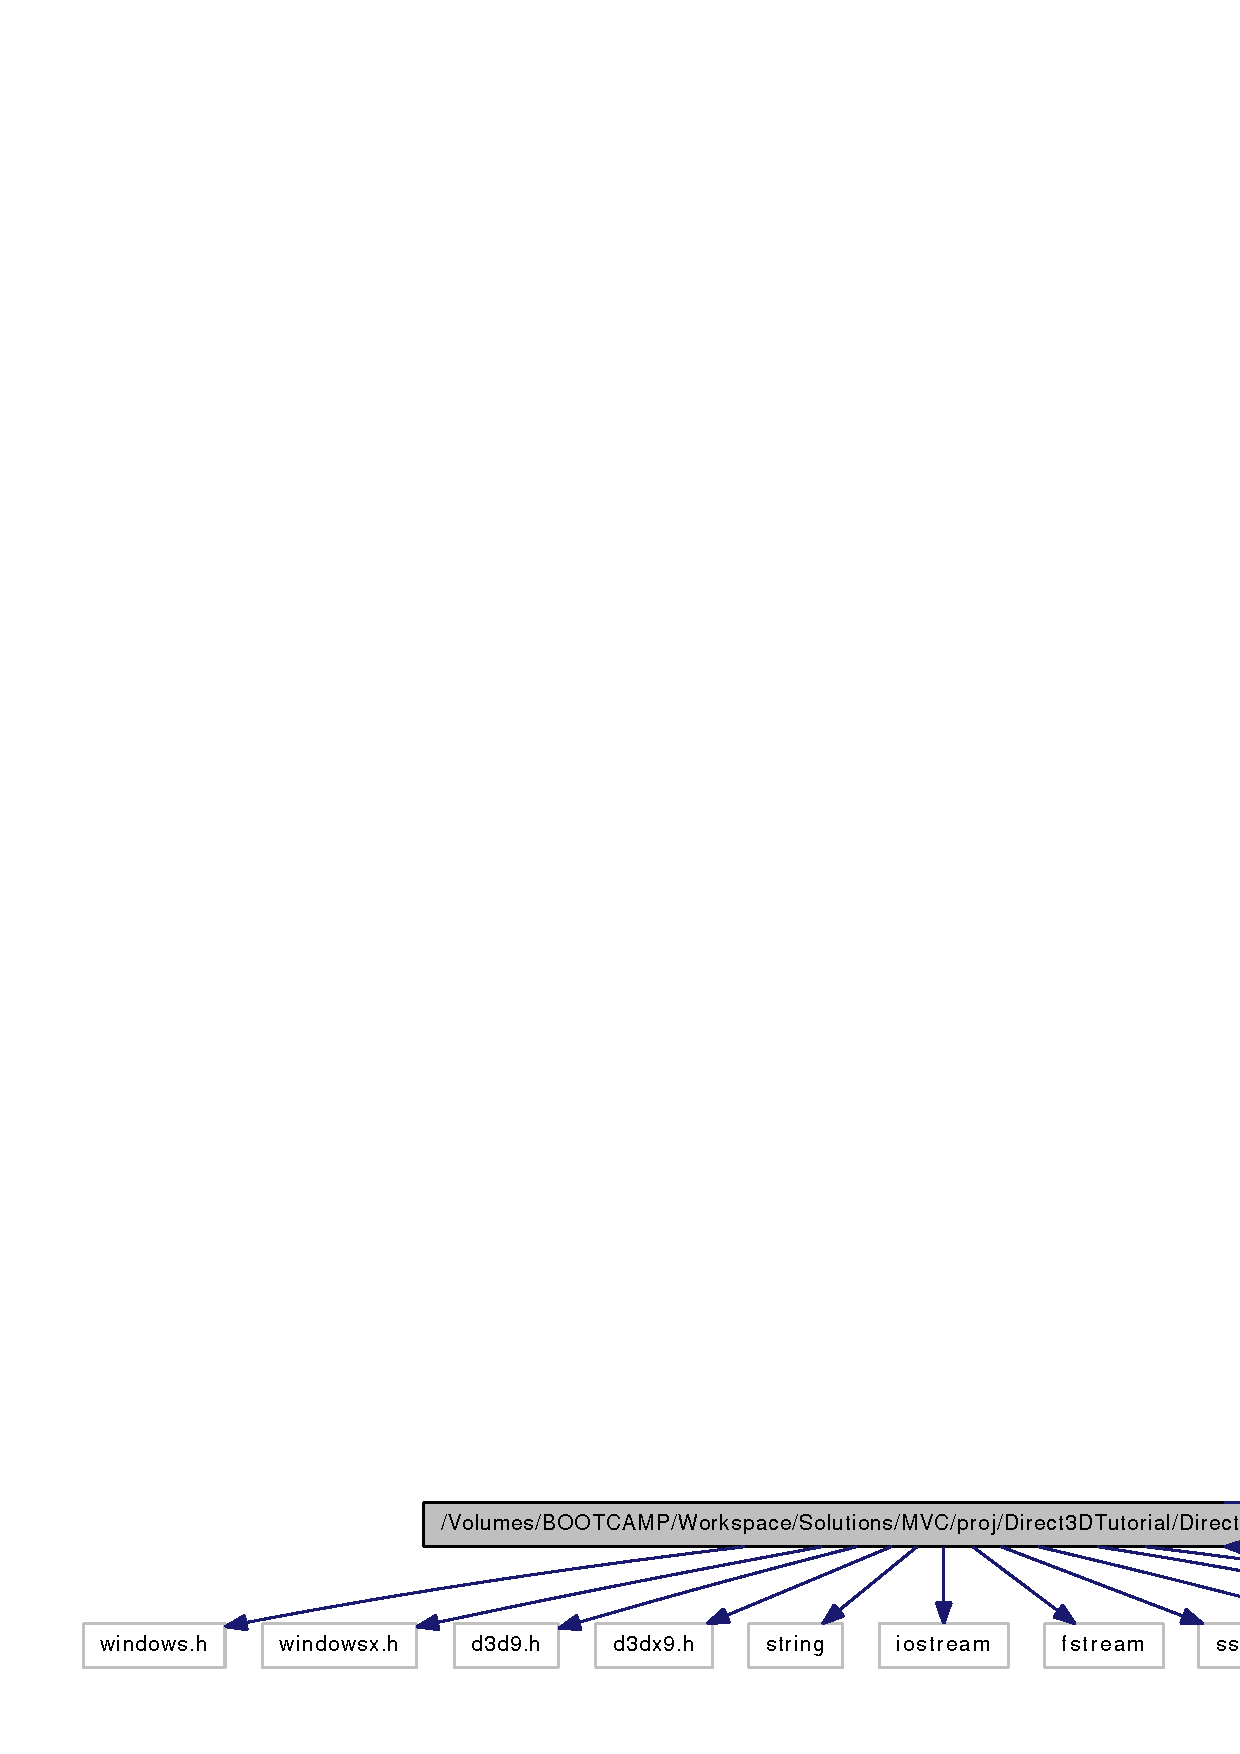
\includegraphics[width=420pt]{main_8cpp__incl}
\end{center}
\end{figure}
This graph shows which files directly or indirectly include this file:\nopagebreak
\begin{figure}[H]
\begin{center}
\leavevmode
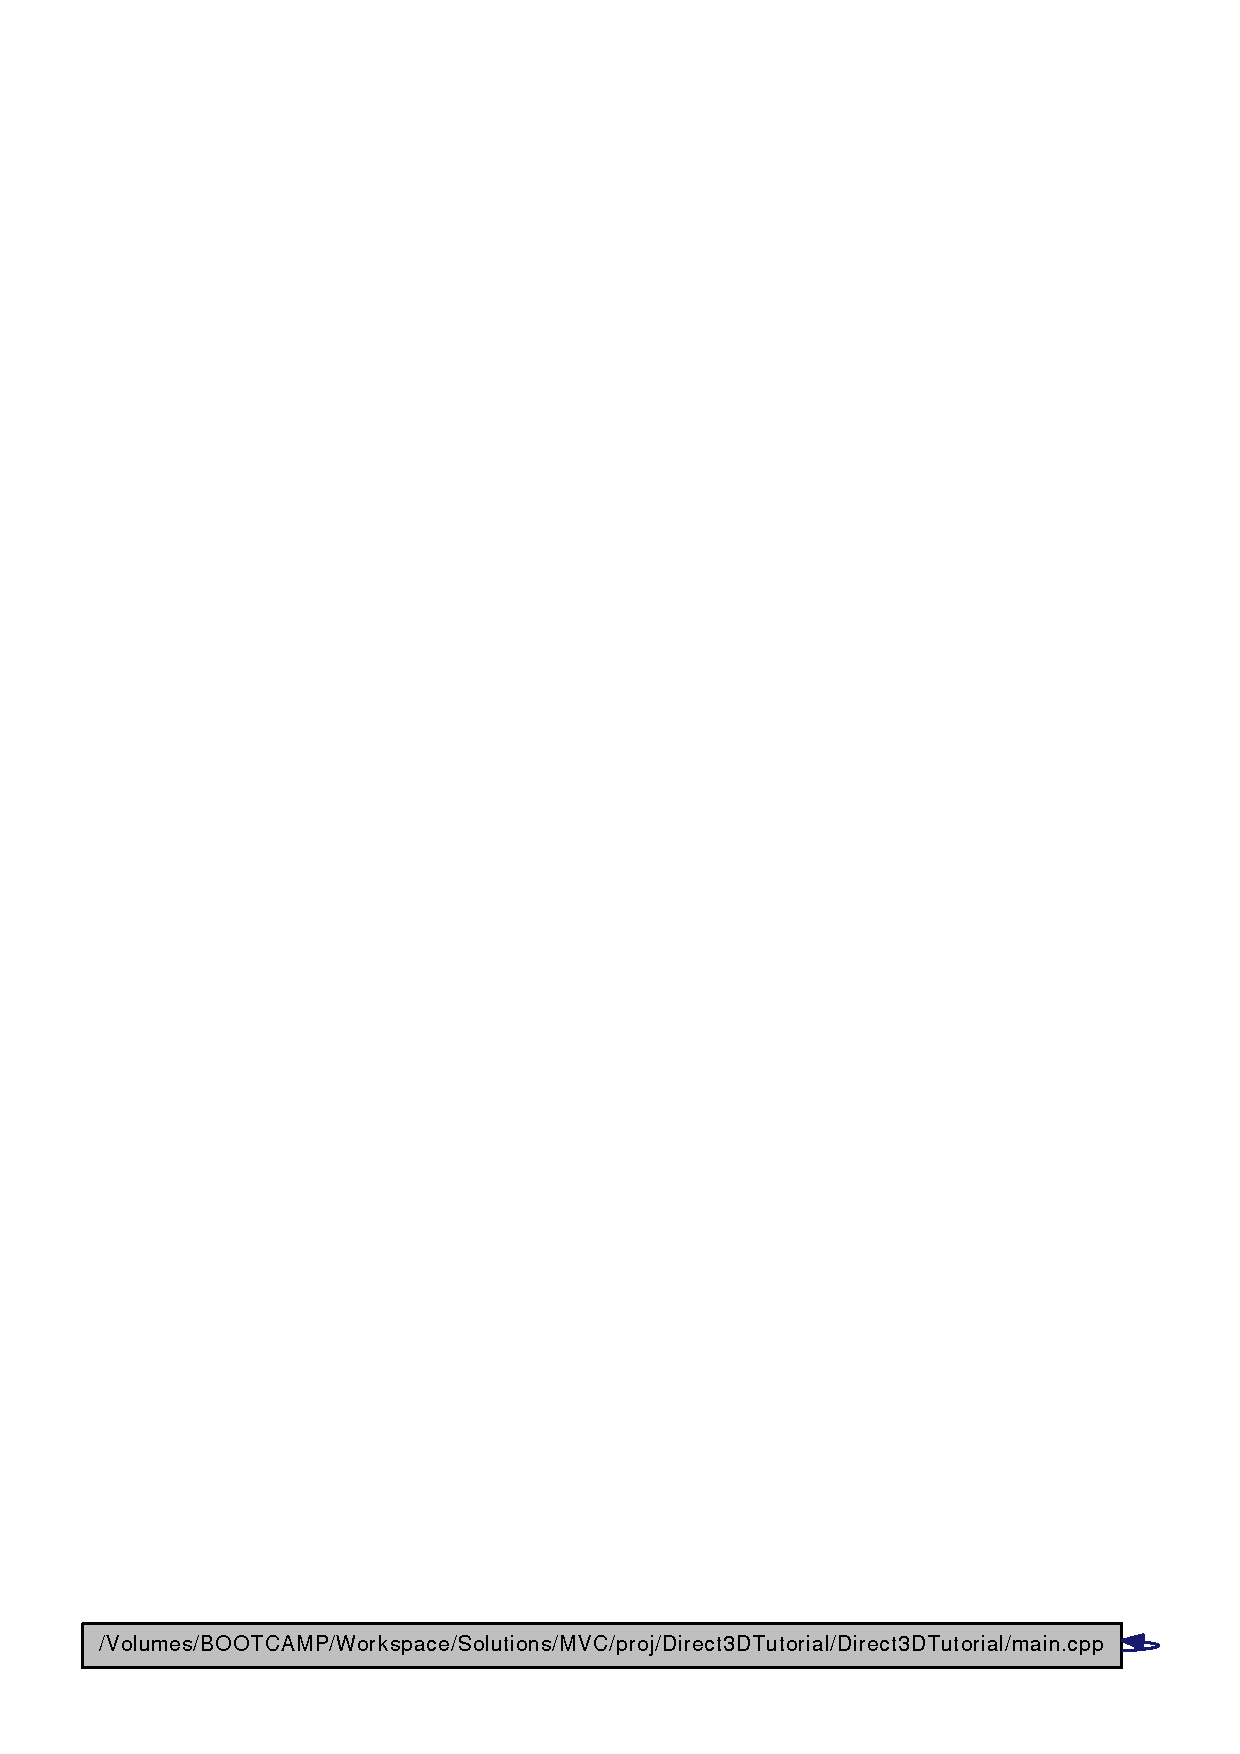
\includegraphics[width=280pt]{main_8cpp__dep__incl}
\end{center}
\end{figure}
\subsection*{Functions}
\begin{DoxyCompactItemize}
\item 
void \hyperlink{main_8cpp_adc57d8d64e4c467f6818cddd81090db7}{initD3D} (HWND hWnd)
\item 
void \hyperlink{main_8cpp_a9d208c9398ed462c31771146011c45a6}{render\_\-frame} (void)
\item 
void \hyperlink{main_8cpp_a6e0493c83a486408dbfaae7812e6e47a}{cleanD3D} (void)
\item 
void \hyperlink{main_8cpp_a6deb2598e68338891c9b1faadea263b9}{getFilename} (int)
\item 
void \hyperlink{main_8cpp_a117a4ee6ce2172cb8d6b4ac48a6c3645}{loadFrame} (int)
\item 
void \hyperlink{main_8cpp_a94b4e3bf0d4387b63e1bc86968b6550d}{render3D} (void)
\item 
LRESULT CALLBACK \hyperlink{main_8cpp_a3481ed5b54326a7e5b2562195ee71a58}{WindowProc} (HWND hWnd, UINT message, WPARAM wParam, LPARAM lParam)
\item 
int WINAPI \hyperlink{main_8cpp_a661c2abc03926acfaeb93b4ae7db4943}{WinMain} (HINSTANCE hInstance, HINSTANCE hPrevInstance, LPSTR lpCmdLine, int nCmdShow)
\item 
wstring \hyperlink{main_8cpp_aad6fe44abbb9cde538b5e84718ee3526}{s2ws} (const string \&s)
\end{DoxyCompactItemize}
\subsection*{Variables}
\begin{DoxyCompactItemize}
\item 
LPDIRECT3D9 \hyperlink{main_8cpp_aa8a3bb0b341846489cc307333d1d9811}{d3d}
\item 
LPDIRECT3DDEVICE9 \hyperlink{main_8cpp_a1c4528473f1127613d4edcaac0dad7f1}{d3ddev}
\item 
IDirect3DSurface9 $\ast$ \hyperlink{main_8cpp_a35944f88a0c5556a08bd1da88b8d89db}{gImageSrc} = NULL
\item 
IDirect3DSurface9 $\ast$ \hyperlink{main_8cpp_a94593fcbf19d34c0830799636182170e}{gBackBuf} = NULL
\item 
RECT \hyperlink{main_8cpp_a908970643424027cd7df53bf68a9cdad}{destRect}
\end{DoxyCompactItemize}


\subsection{Function Documentation}
\hypertarget{main_8cpp_a6e0493c83a486408dbfaae7812e6e47a}{
\index{main.cpp@{main.cpp}!cleanD3D@{cleanD3D}}
\index{cleanD3D@{cleanD3D}!main.cpp@{main.cpp}}
\subsubsection[{cleanD3D}]{\setlength{\rightskip}{0pt plus 5cm}void cleanD3D (void)}}
\label{main_8cpp_a6e0493c83a486408dbfaae7812e6e47a}


Definition at line \hyperlink{main_8cpp_source_l00255}{255} of file \hyperlink{main_8cpp_source}{main.cpp}.



Here is the caller graph for this function:\nopagebreak
\begin{figure}[H]
\begin{center}
\leavevmode
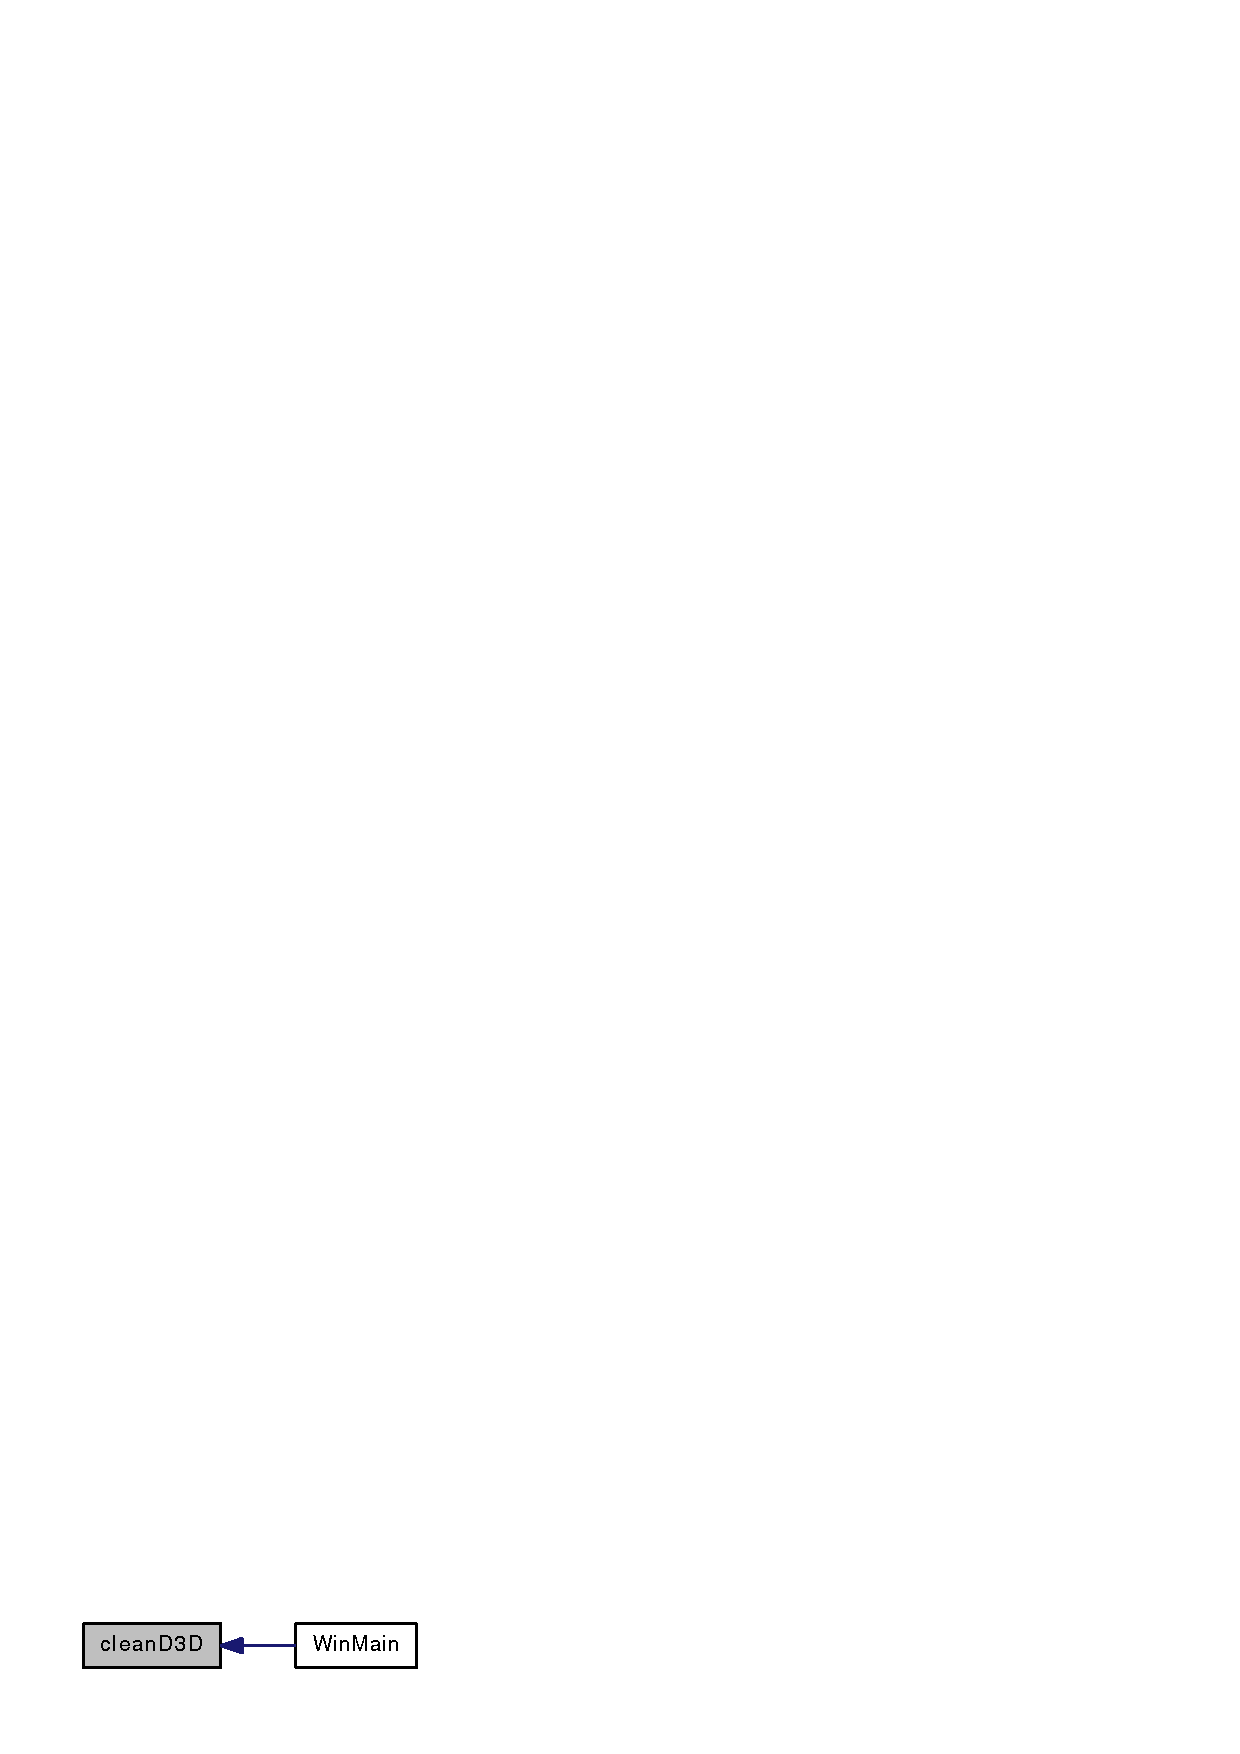
\includegraphics[width=102pt]{main_8cpp_a6e0493c83a486408dbfaae7812e6e47a_icgraph}
\end{center}
\end{figure}


\hypertarget{main_8cpp_a6deb2598e68338891c9b1faadea263b9}{
\index{main.cpp@{main.cpp}!getFilename@{getFilename}}
\index{getFilename@{getFilename}!main.cpp@{main.cpp}}
\subsubsection[{getFilename}]{\setlength{\rightskip}{0pt plus 5cm}void getFilename (int {\em \_\-frame})}}
\label{main_8cpp_a6deb2598e68338891c9b1faadea263b9}


Definition at line \hyperlink{main_8cpp_source_l00285}{285} of file \hyperlink{main_8cpp_source}{main.cpp}.



Here is the call graph for this function:\nopagebreak
\begin{figure}[H]
\begin{center}
\leavevmode
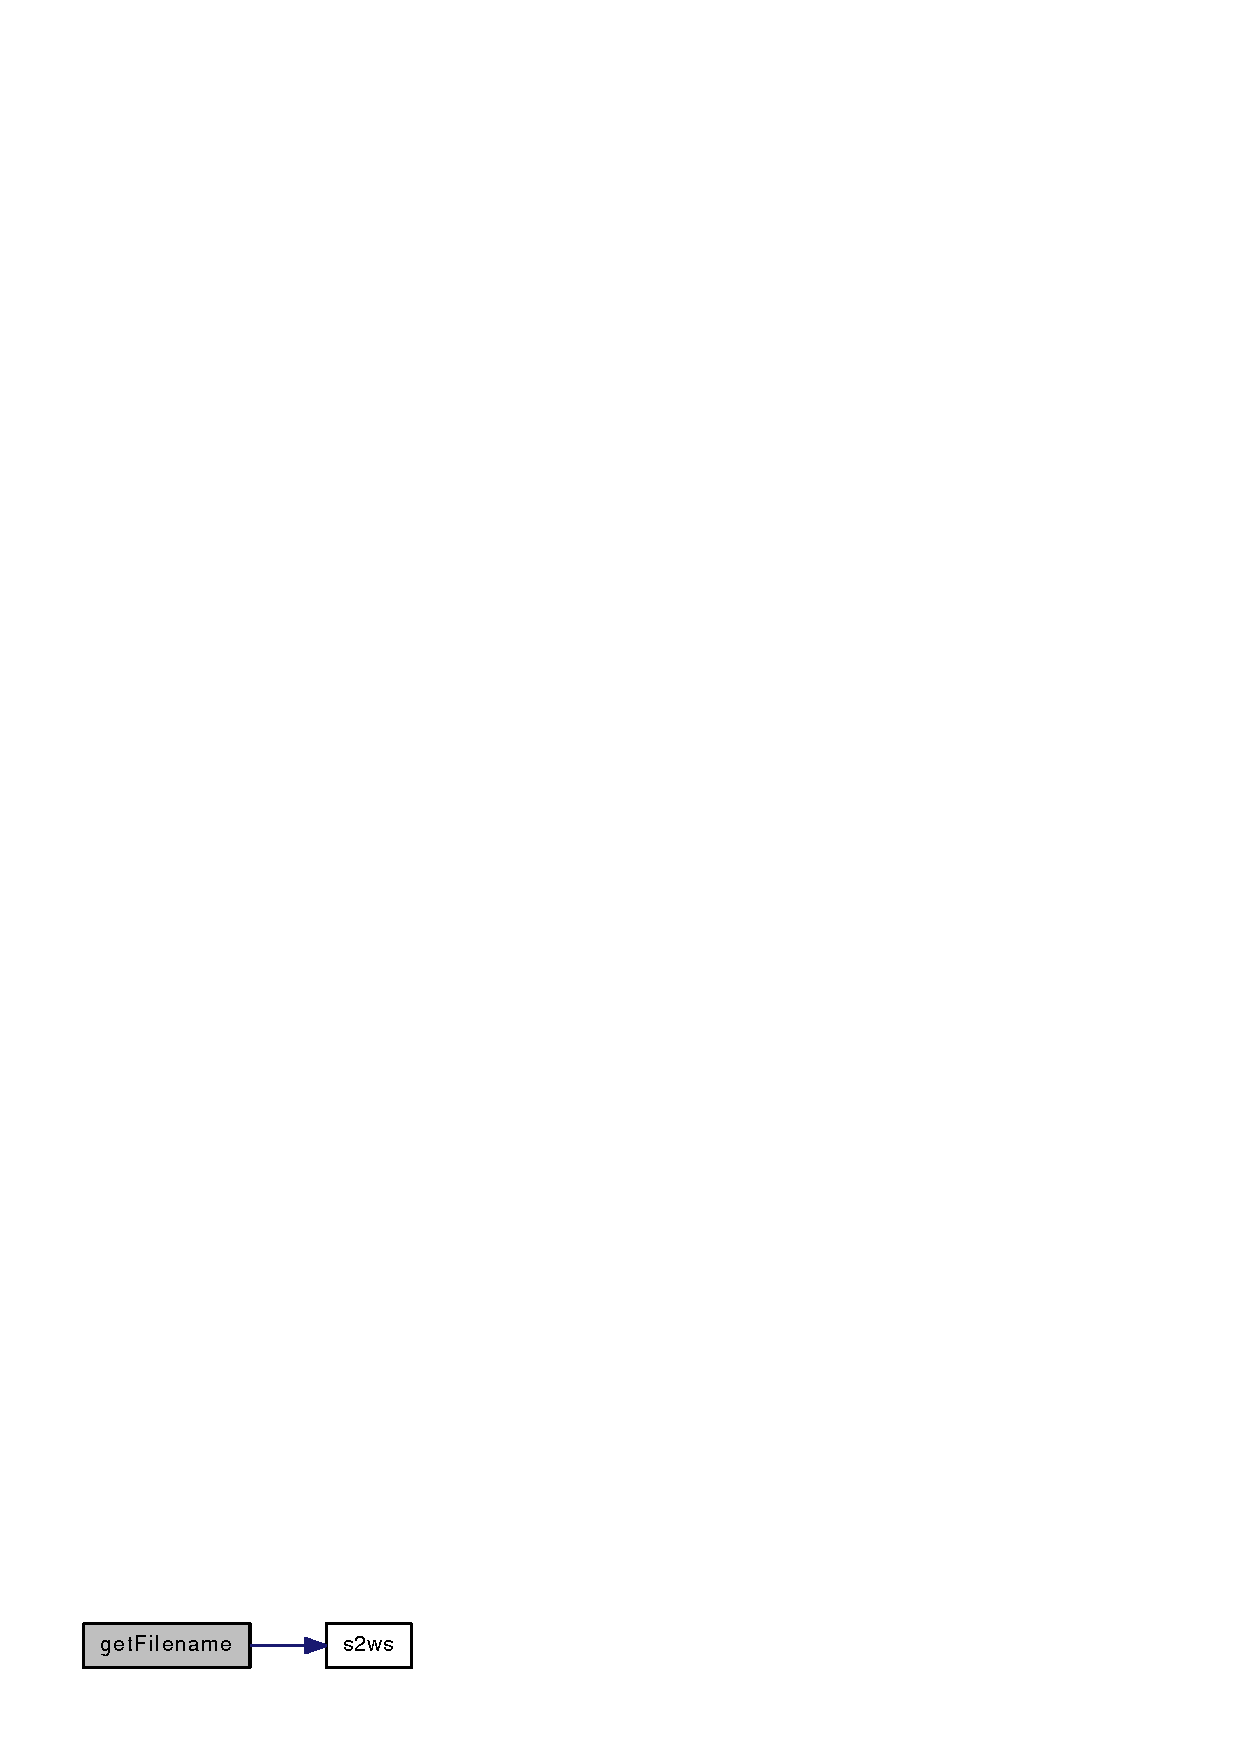
\includegraphics[width=101pt]{main_8cpp_a6deb2598e68338891c9b1faadea263b9_cgraph}
\end{center}
\end{figure}




Here is the caller graph for this function:\nopagebreak
\begin{figure}[H]
\begin{center}
\leavevmode
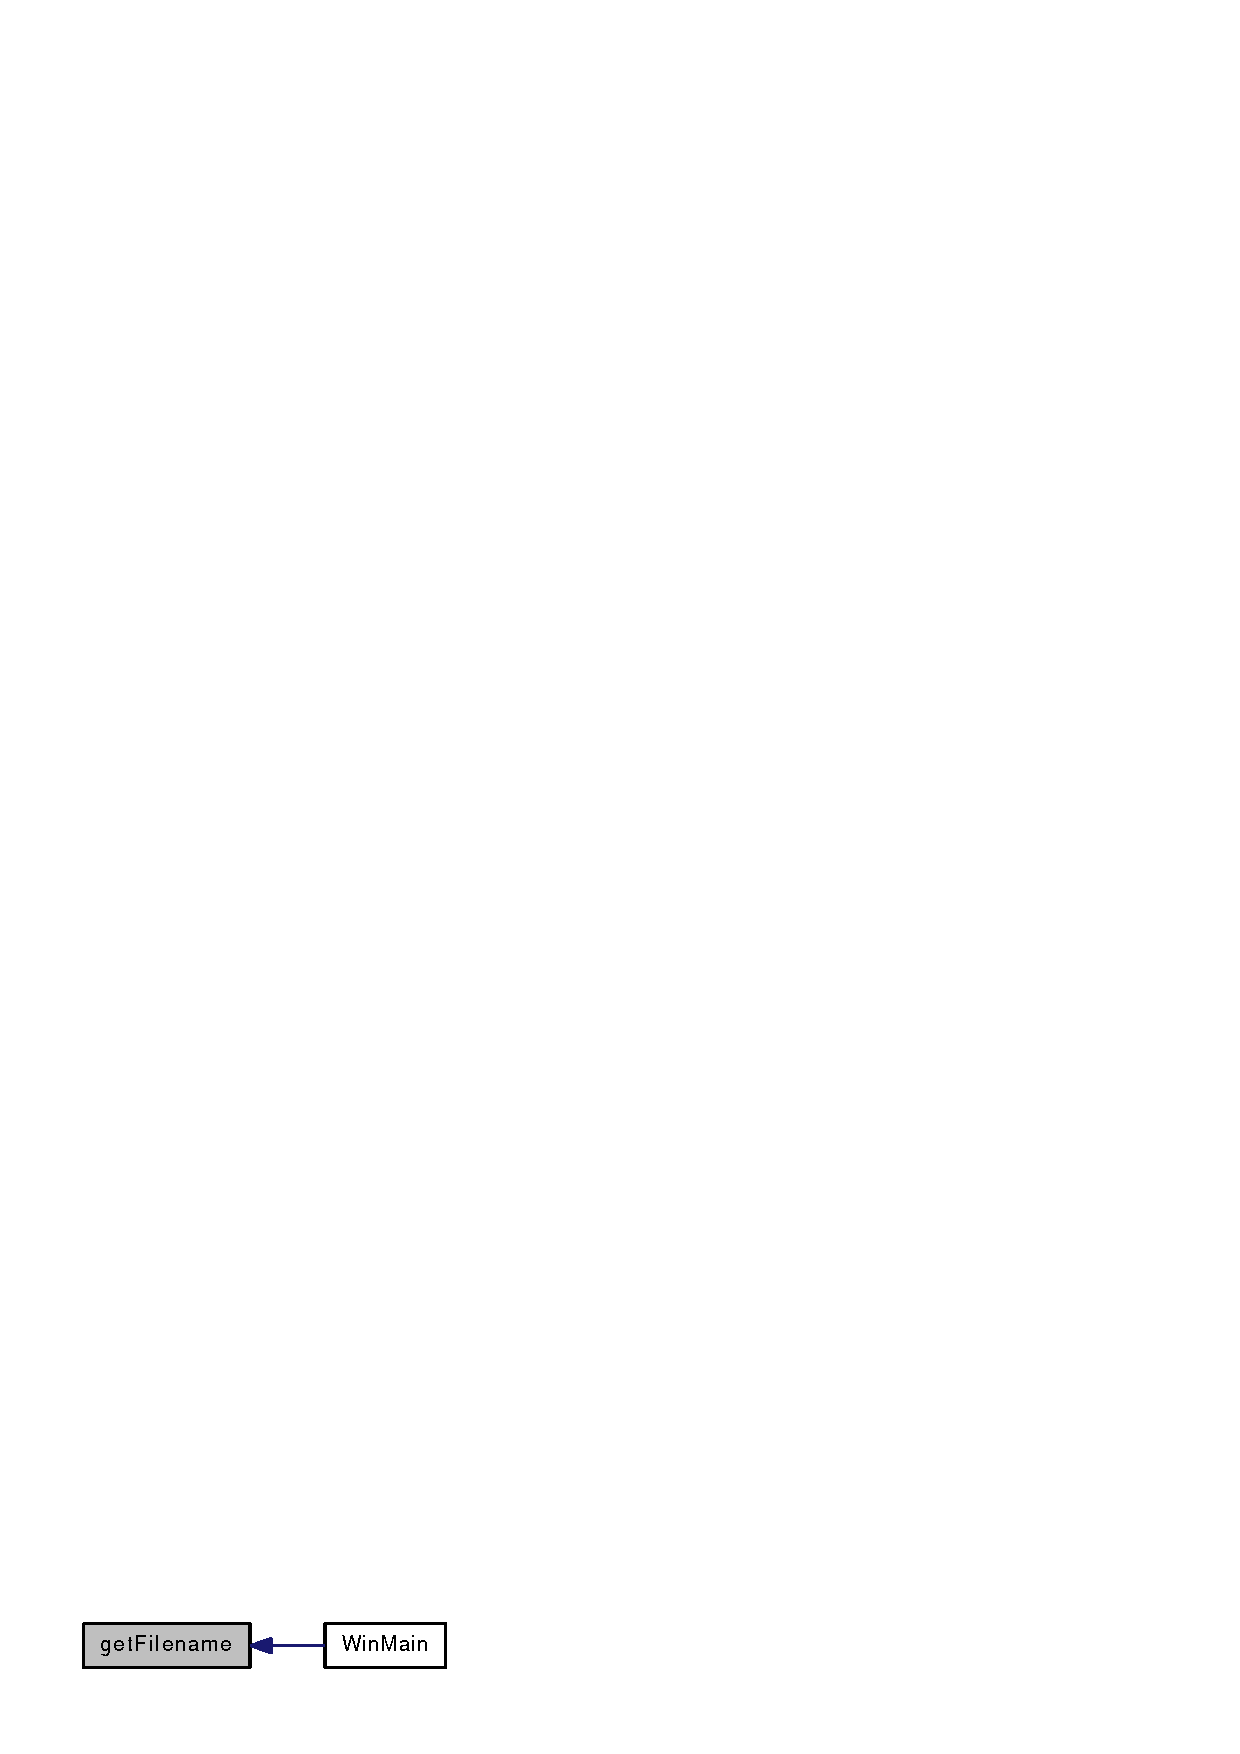
\includegraphics[width=109pt]{main_8cpp_a6deb2598e68338891c9b1faadea263b9_icgraph}
\end{center}
\end{figure}


\hypertarget{main_8cpp_adc57d8d64e4c467f6818cddd81090db7}{
\index{main.cpp@{main.cpp}!initD3D@{initD3D}}
\index{initD3D@{initD3D}!main.cpp@{main.cpp}}
\subsubsection[{initD3D}]{\setlength{\rightskip}{0pt plus 5cm}void initD3D (HWND {\em hWnd})}}
\label{main_8cpp_adc57d8d64e4c467f6818cddd81090db7}


Definition at line \hyperlink{main_8cpp_source_l00218}{218} of file \hyperlink{main_8cpp_source}{main.cpp}.



Here is the caller graph for this function:\nopagebreak
\begin{figure}[H]
\begin{center}
\leavevmode
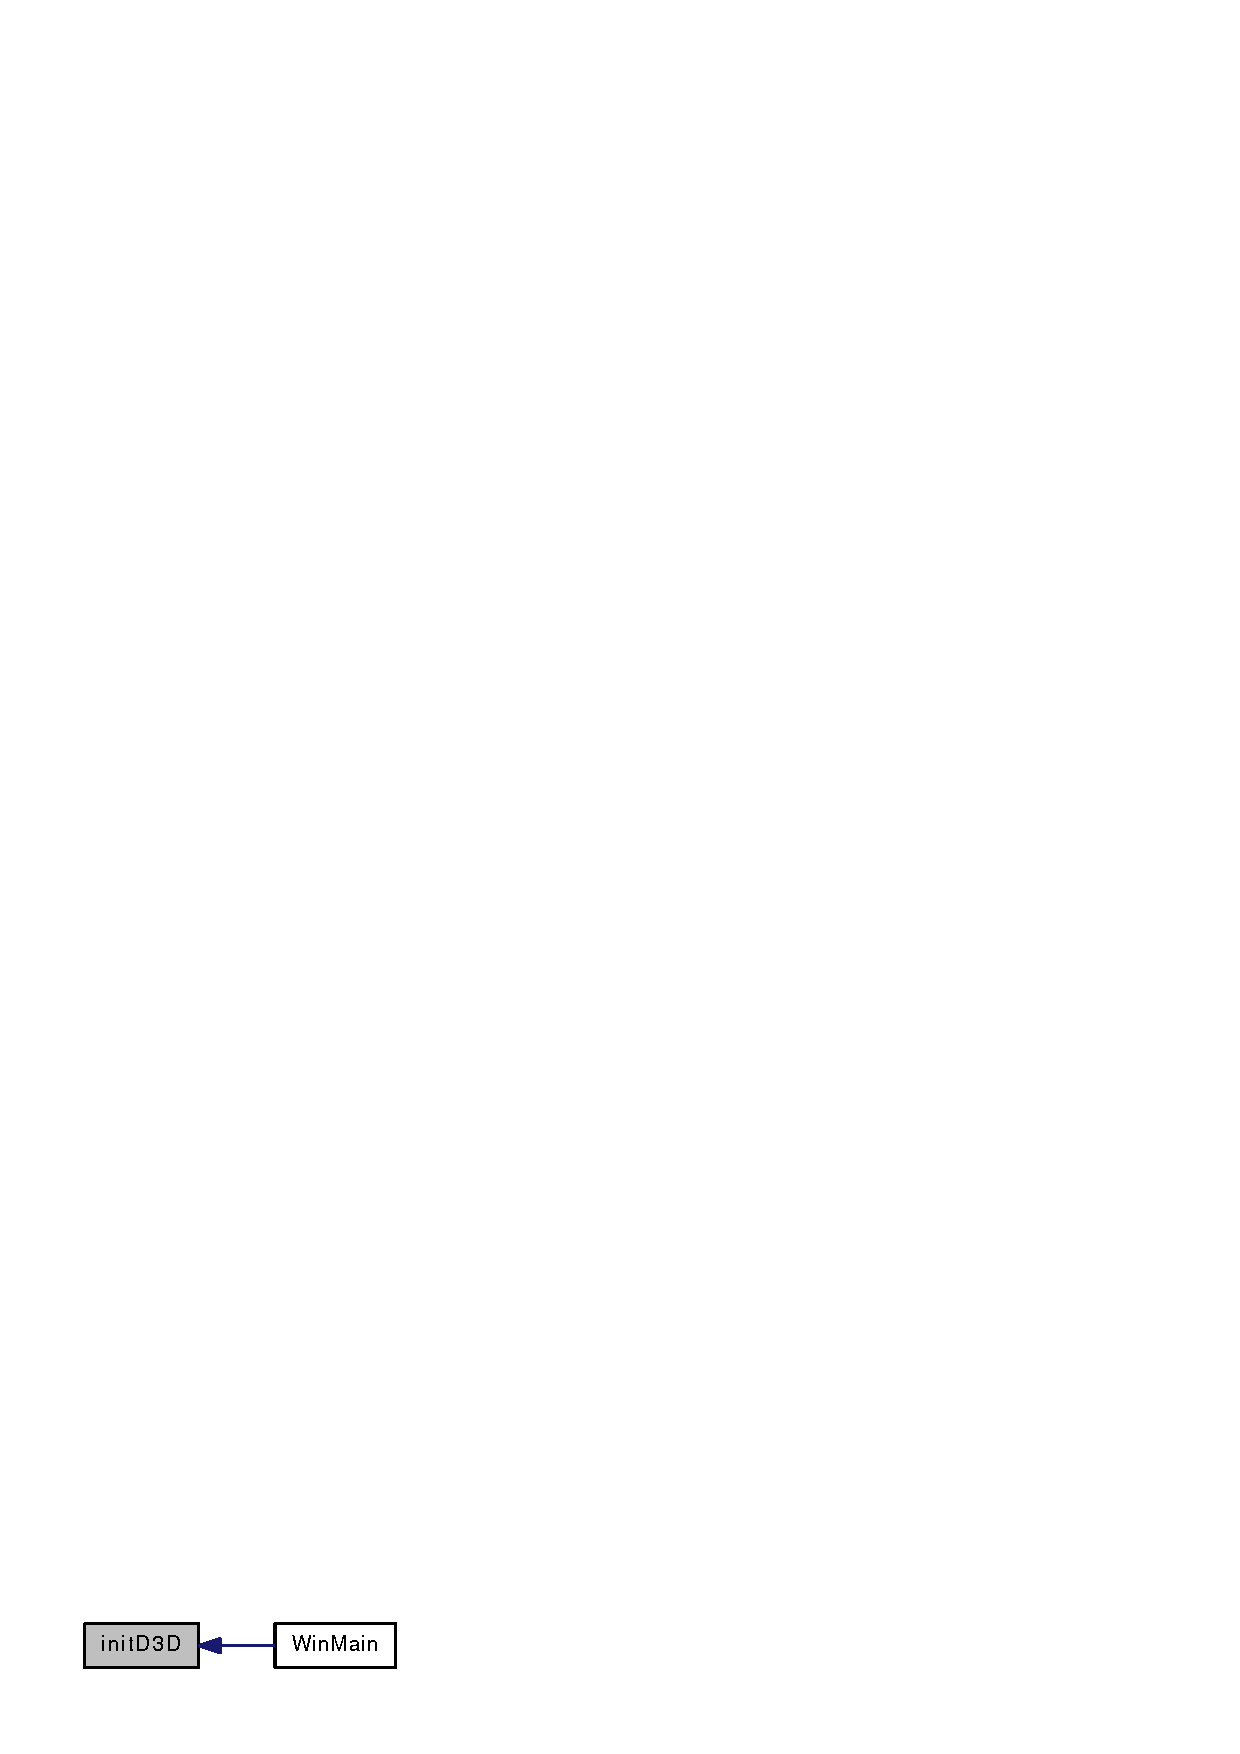
\includegraphics[width=97pt]{main_8cpp_adc57d8d64e4c467f6818cddd81090db7_icgraph}
\end{center}
\end{figure}


\hypertarget{main_8cpp_a117a4ee6ce2172cb8d6b4ac48a6c3645}{
\index{main.cpp@{main.cpp}!loadFrame@{loadFrame}}
\index{loadFrame@{loadFrame}!main.cpp@{main.cpp}}
\subsubsection[{loadFrame}]{\setlength{\rightskip}{0pt plus 5cm}void loadFrame (int {\em \_\-frame})}}
\label{main_8cpp_a117a4ee6ce2172cb8d6b4ac48a6c3645}


$\ast$ 



Definition at line \hyperlink{main_8cpp_source_l00306}{306} of file \hyperlink{main_8cpp_source}{main.cpp}.



Here is the caller graph for this function:\nopagebreak
\begin{figure}[H]
\begin{center}
\leavevmode
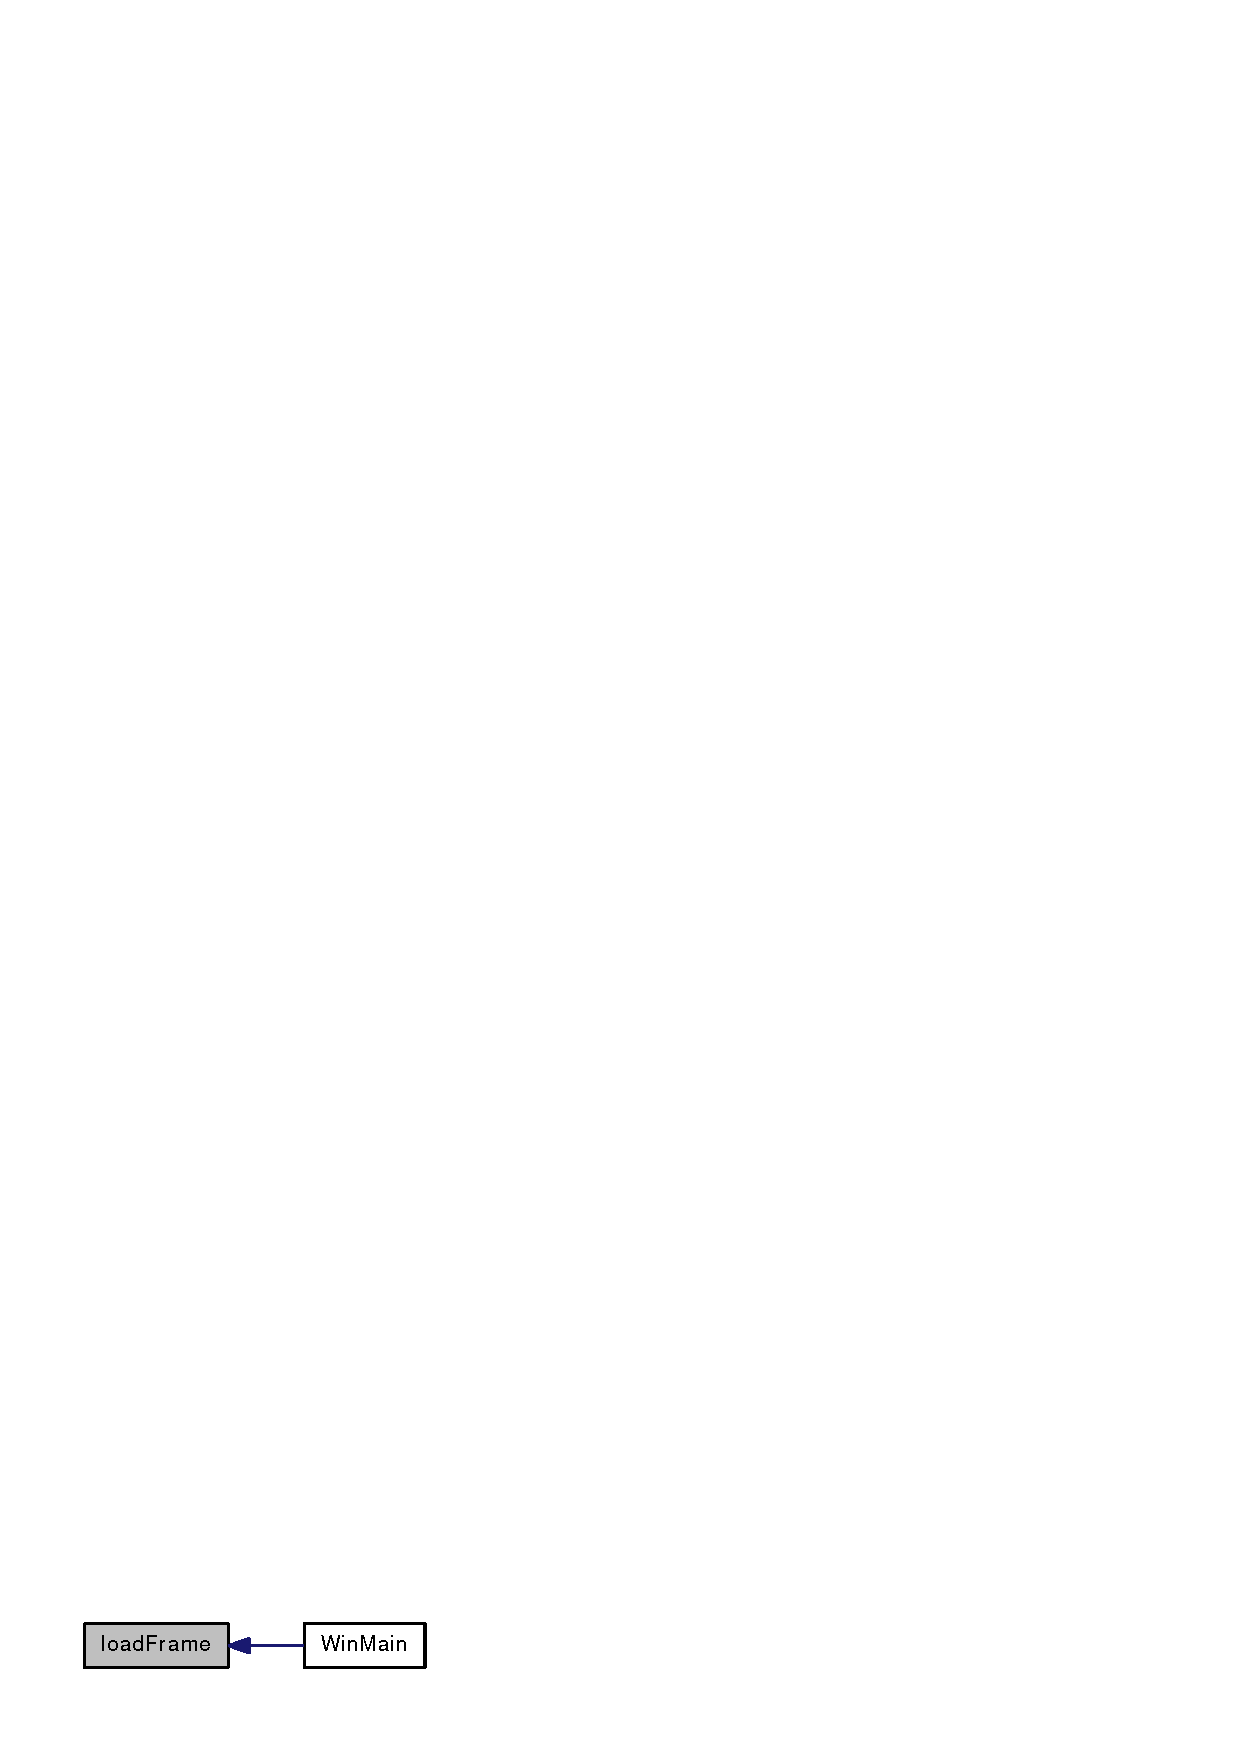
\includegraphics[width=104pt]{main_8cpp_a117a4ee6ce2172cb8d6b4ac48a6c3645_icgraph}
\end{center}
\end{figure}


\hypertarget{main_8cpp_a94b4e3bf0d4387b63e1bc86968b6550d}{
\index{main.cpp@{main.cpp}!render3D@{render3D}}
\index{render3D@{render3D}!main.cpp@{main.cpp}}
\subsubsection[{render3D}]{\setlength{\rightskip}{0pt plus 5cm}void render3D (void)}}
\label{main_8cpp_a94b4e3bf0d4387b63e1bc86968b6550d}


Definition at line \hyperlink{main_8cpp_source_l00262}{262} of file \hyperlink{main_8cpp_source}{main.cpp}.



Here is the caller graph for this function:\nopagebreak
\begin{figure}[H]
\begin{center}
\leavevmode
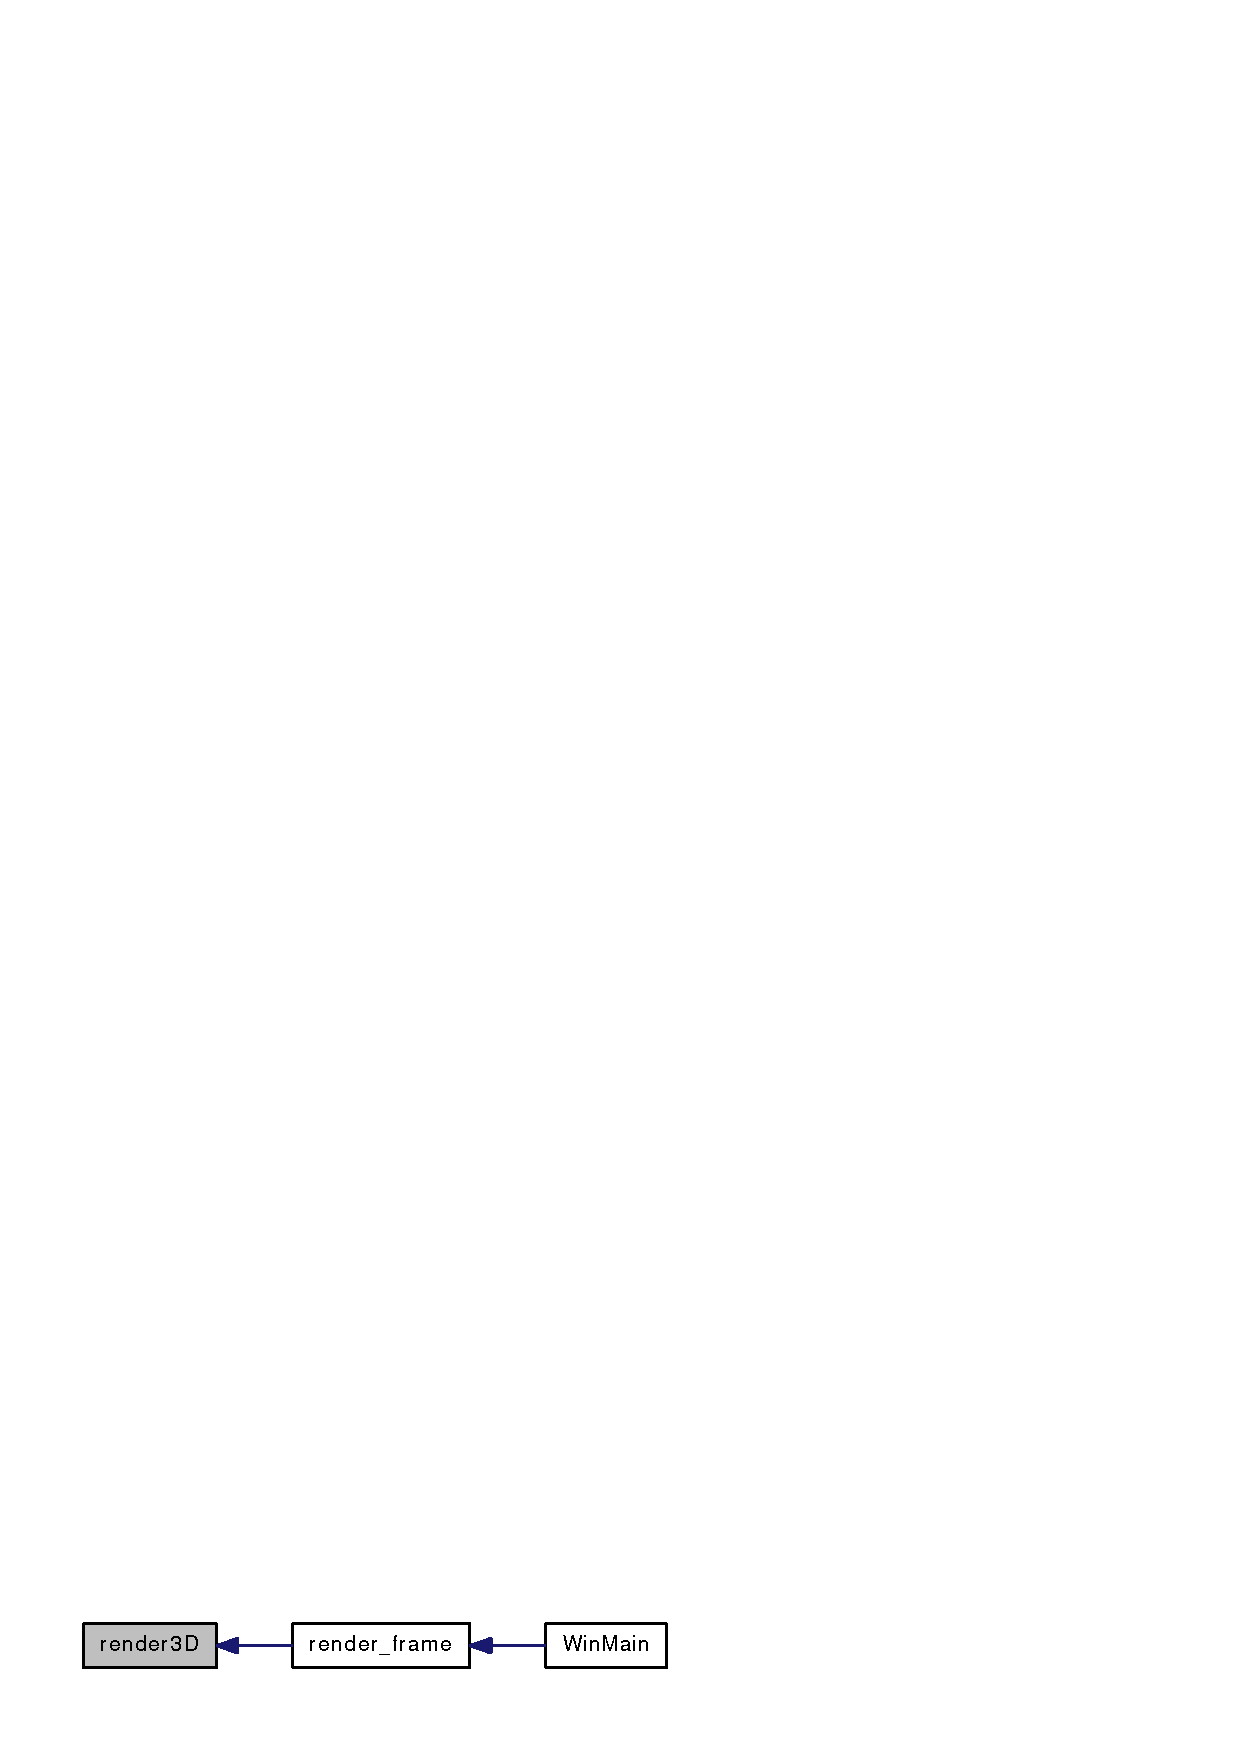
\includegraphics[width=162pt]{main_8cpp_a94b4e3bf0d4387b63e1bc86968b6550d_icgraph}
\end{center}
\end{figure}


\hypertarget{main_8cpp_a9d208c9398ed462c31771146011c45a6}{
\index{main.cpp@{main.cpp}!render\_\-frame@{render\_\-frame}}
\index{render\_\-frame@{render\_\-frame}!main.cpp@{main.cpp}}
\subsubsection[{render\_\-frame}]{\setlength{\rightskip}{0pt plus 5cm}void render\_\-frame (void)}}
\label{main_8cpp_a9d208c9398ed462c31771146011c45a6}


Definition at line \hyperlink{main_8cpp_source_l00238}{238} of file \hyperlink{main_8cpp_source}{main.cpp}.



Here is the call graph for this function:\nopagebreak
\begin{figure}[H]
\begin{center}
\leavevmode
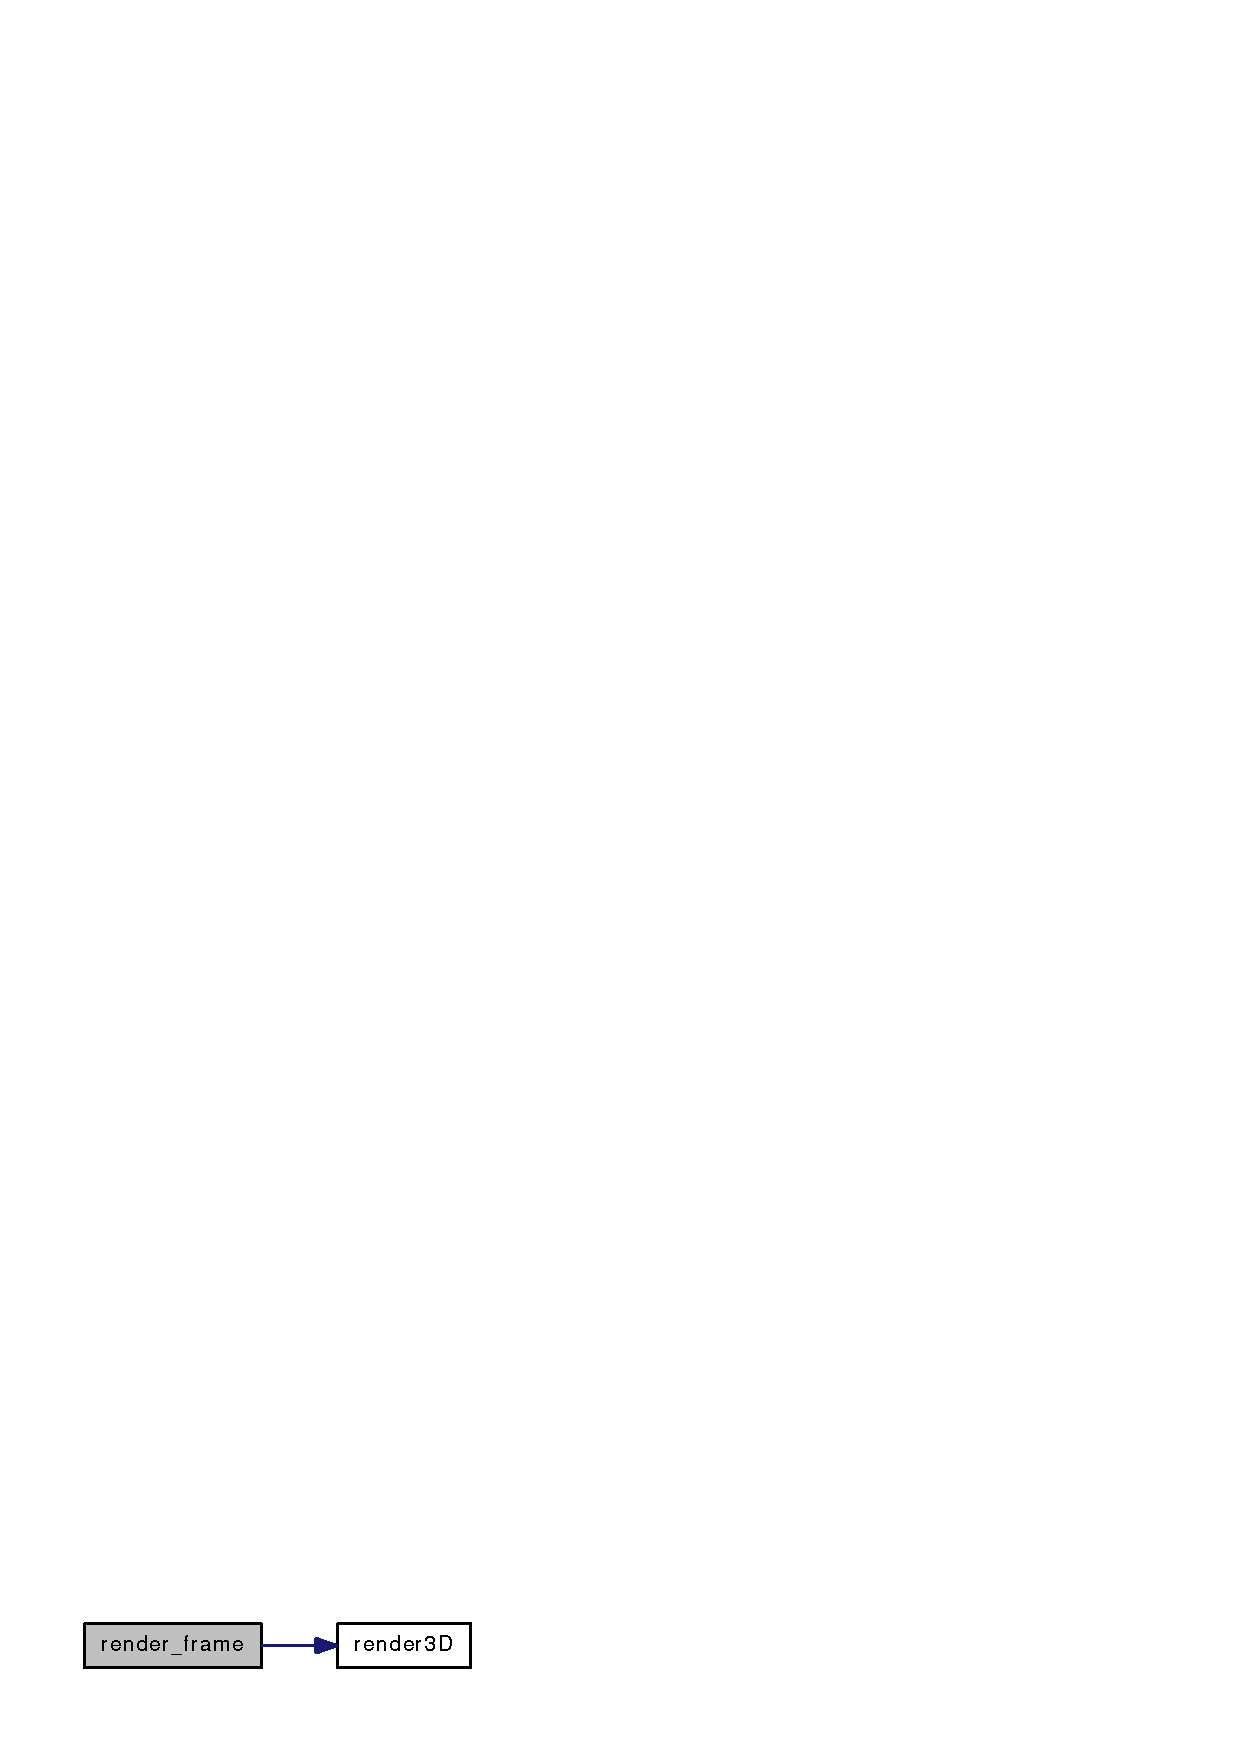
\includegraphics[width=115pt]{main_8cpp_a9d208c9398ed462c31771146011c45a6_cgraph}
\end{center}
\end{figure}




Here is the caller graph for this function:\nopagebreak
\begin{figure}[H]
\begin{center}
\leavevmode
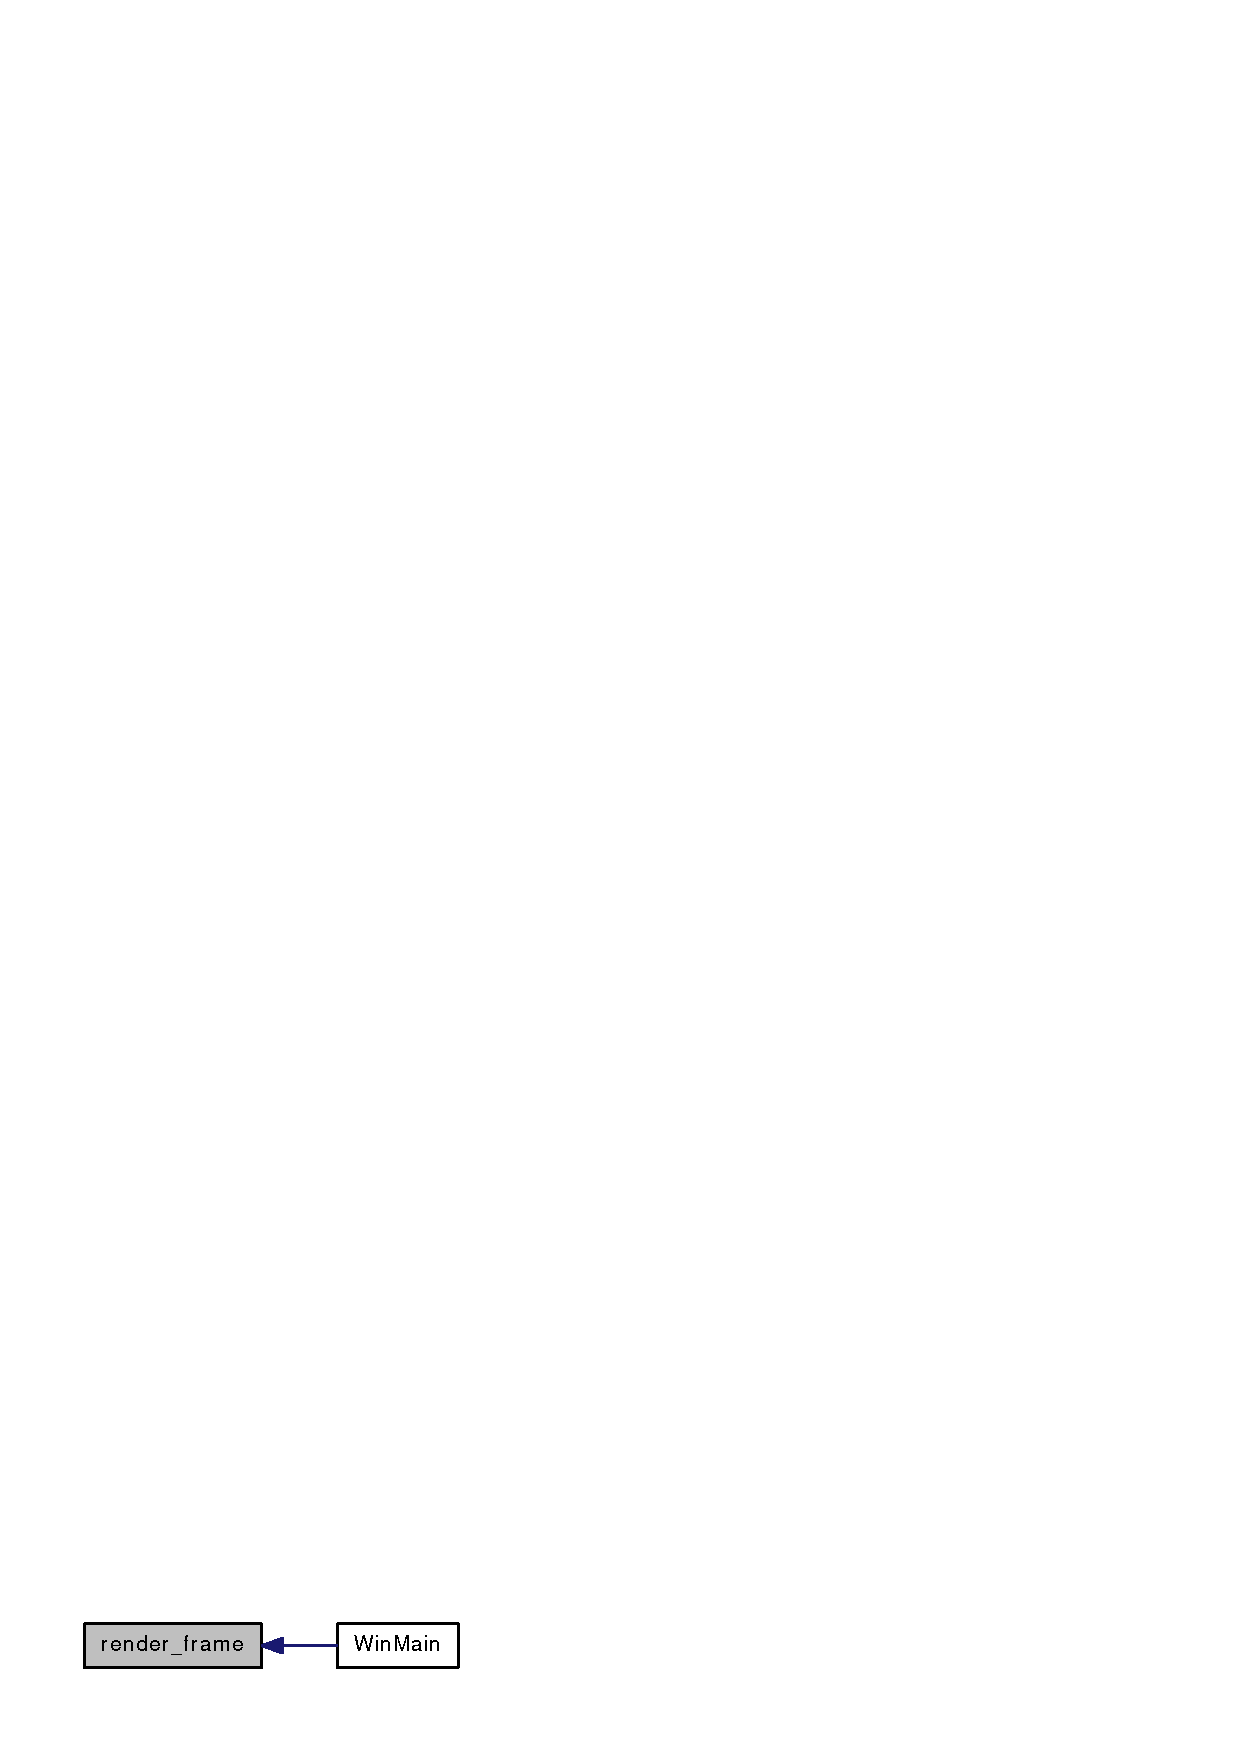
\includegraphics[width=112pt]{main_8cpp_a9d208c9398ed462c31771146011c45a6_icgraph}
\end{center}
\end{figure}


\hypertarget{main_8cpp_aad6fe44abbb9cde538b5e84718ee3526}{
\index{main.cpp@{main.cpp}!s2ws@{s2ws}}
\index{s2ws@{s2ws}!main.cpp@{main.cpp}}
\subsubsection[{s2ws}]{\setlength{\rightskip}{0pt plus 5cm}wstring s2ws (const string \& {\em s})}}
\label{main_8cpp_aad6fe44abbb9cde538b5e84718ee3526}


Definition at line \hyperlink{main_8cpp_source_l00274}{274} of file \hyperlink{main_8cpp_source}{main.cpp}.



Here is the caller graph for this function:\nopagebreak
\begin{figure}[H]
\begin{center}
\leavevmode
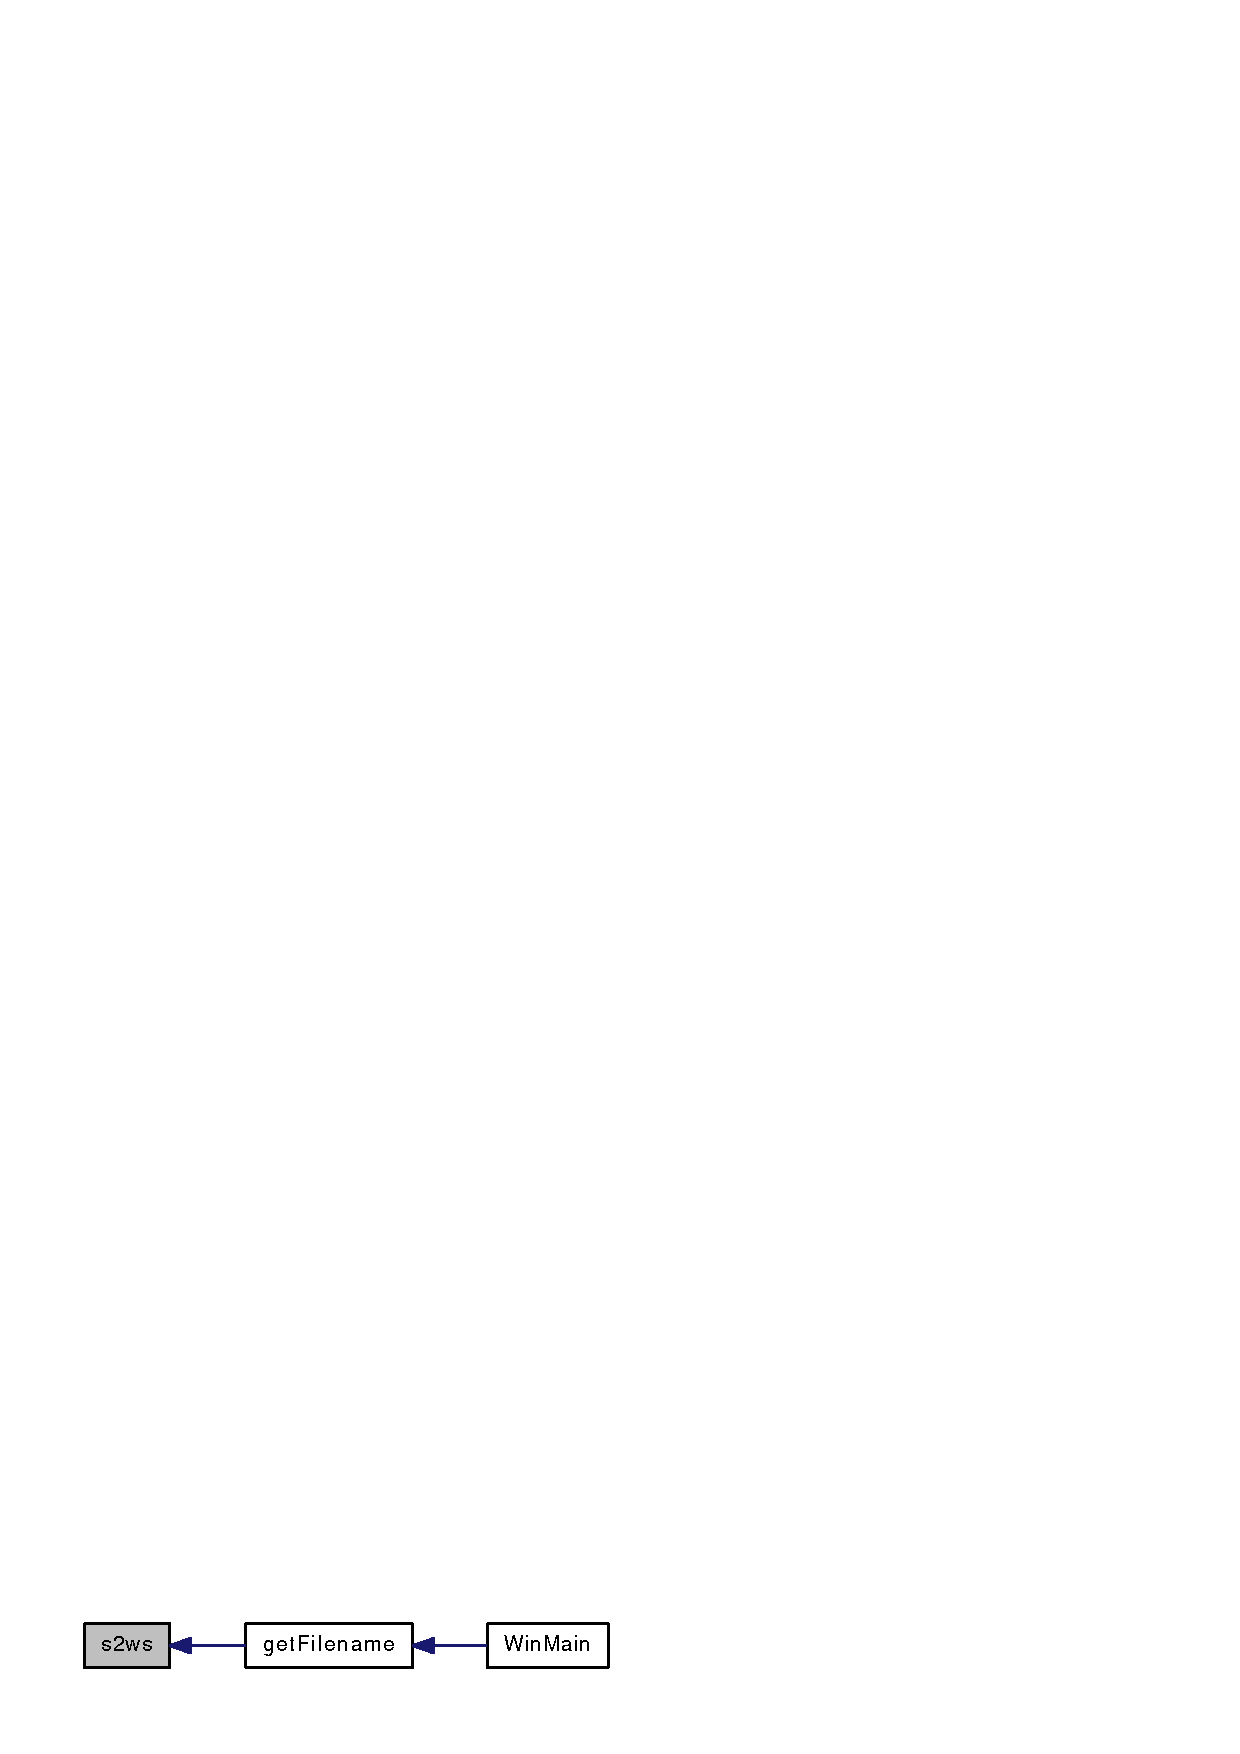
\includegraphics[width=148pt]{main_8cpp_aad6fe44abbb9cde538b5e84718ee3526_icgraph}
\end{center}
\end{figure}


\hypertarget{main_8cpp_a3481ed5b54326a7e5b2562195ee71a58}{
\index{main.cpp@{main.cpp}!WindowProc@{WindowProc}}
\index{WindowProc@{WindowProc}!main.cpp@{main.cpp}}
\subsubsection[{WindowProc}]{\setlength{\rightskip}{0pt plus 5cm}LRESULT CALLBACK WindowProc (HWND {\em hWnd}, \/  UINT {\em message}, \/  WPARAM {\em wParam}, \/  LPARAM {\em lParam})}}
\label{main_8cpp_a3481ed5b54326a7e5b2562195ee71a58}


Definition at line \hyperlink{main_8cpp_source_l00201}{201} of file \hyperlink{main_8cpp_source}{main.cpp}.



Here is the caller graph for this function:\nopagebreak
\begin{figure}[H]
\begin{center}
\leavevmode
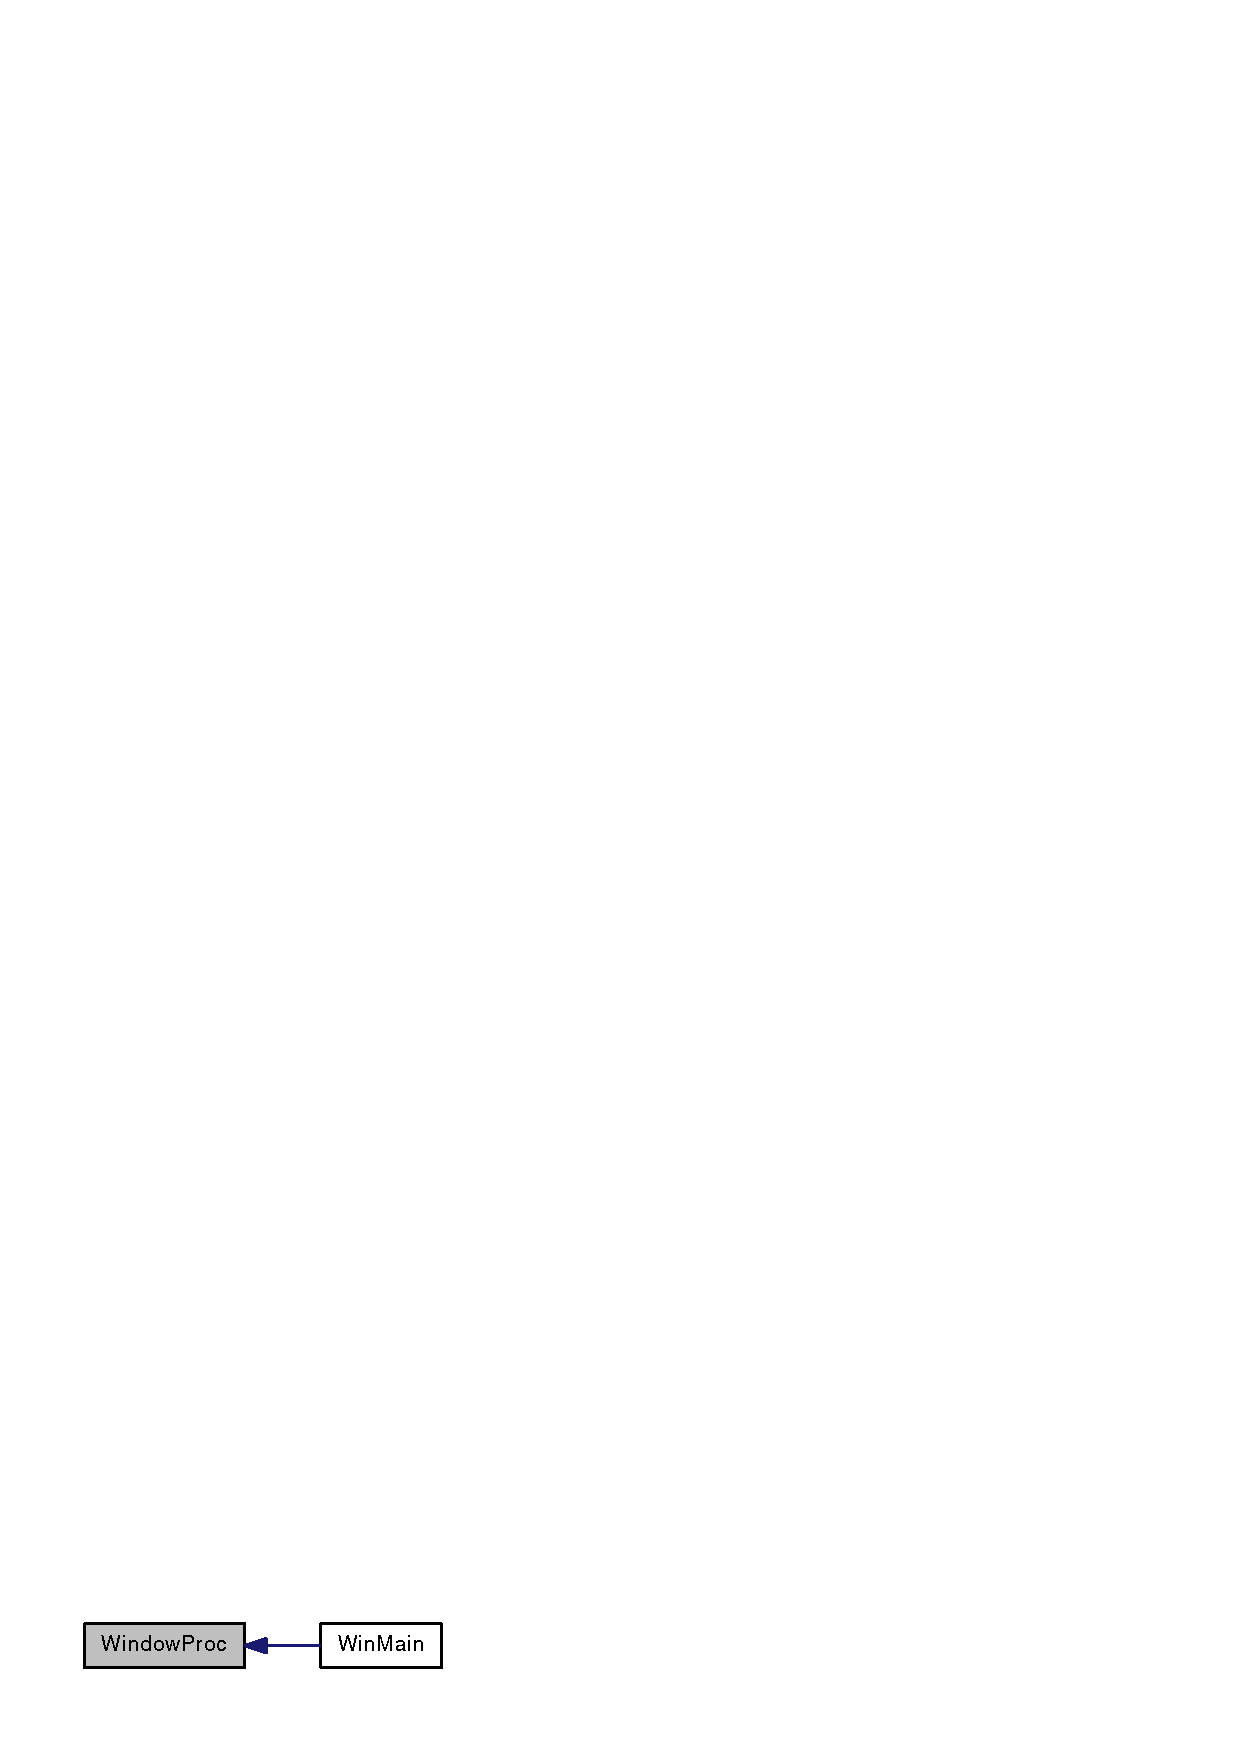
\includegraphics[width=108pt]{main_8cpp_a3481ed5b54326a7e5b2562195ee71a58_icgraph}
\end{center}
\end{figure}


\hypertarget{main_8cpp_a661c2abc03926acfaeb93b4ae7db4943}{
\index{main.cpp@{main.cpp}!WinMain@{WinMain}}
\index{WinMain@{WinMain}!main.cpp@{main.cpp}}
\subsubsection[{WinMain}]{\setlength{\rightskip}{0pt plus 5cm}int WINAPI WinMain (HINSTANCE {\em hInstance}, \/  HINSTANCE {\em hPrevInstance}, \/  LPSTR {\em lpCmdLine}, \/  int {\em nCmdShow})}}
\label{main_8cpp_a661c2abc03926acfaeb93b4ae7db4943}


Definition at line \hyperlink{main_8cpp_source_l00046}{46} of file \hyperlink{main_8cpp_source}{main.cpp}.



Here is the call graph for this function:\nopagebreak
\begin{figure}[H]
\begin{center}
\leavevmode
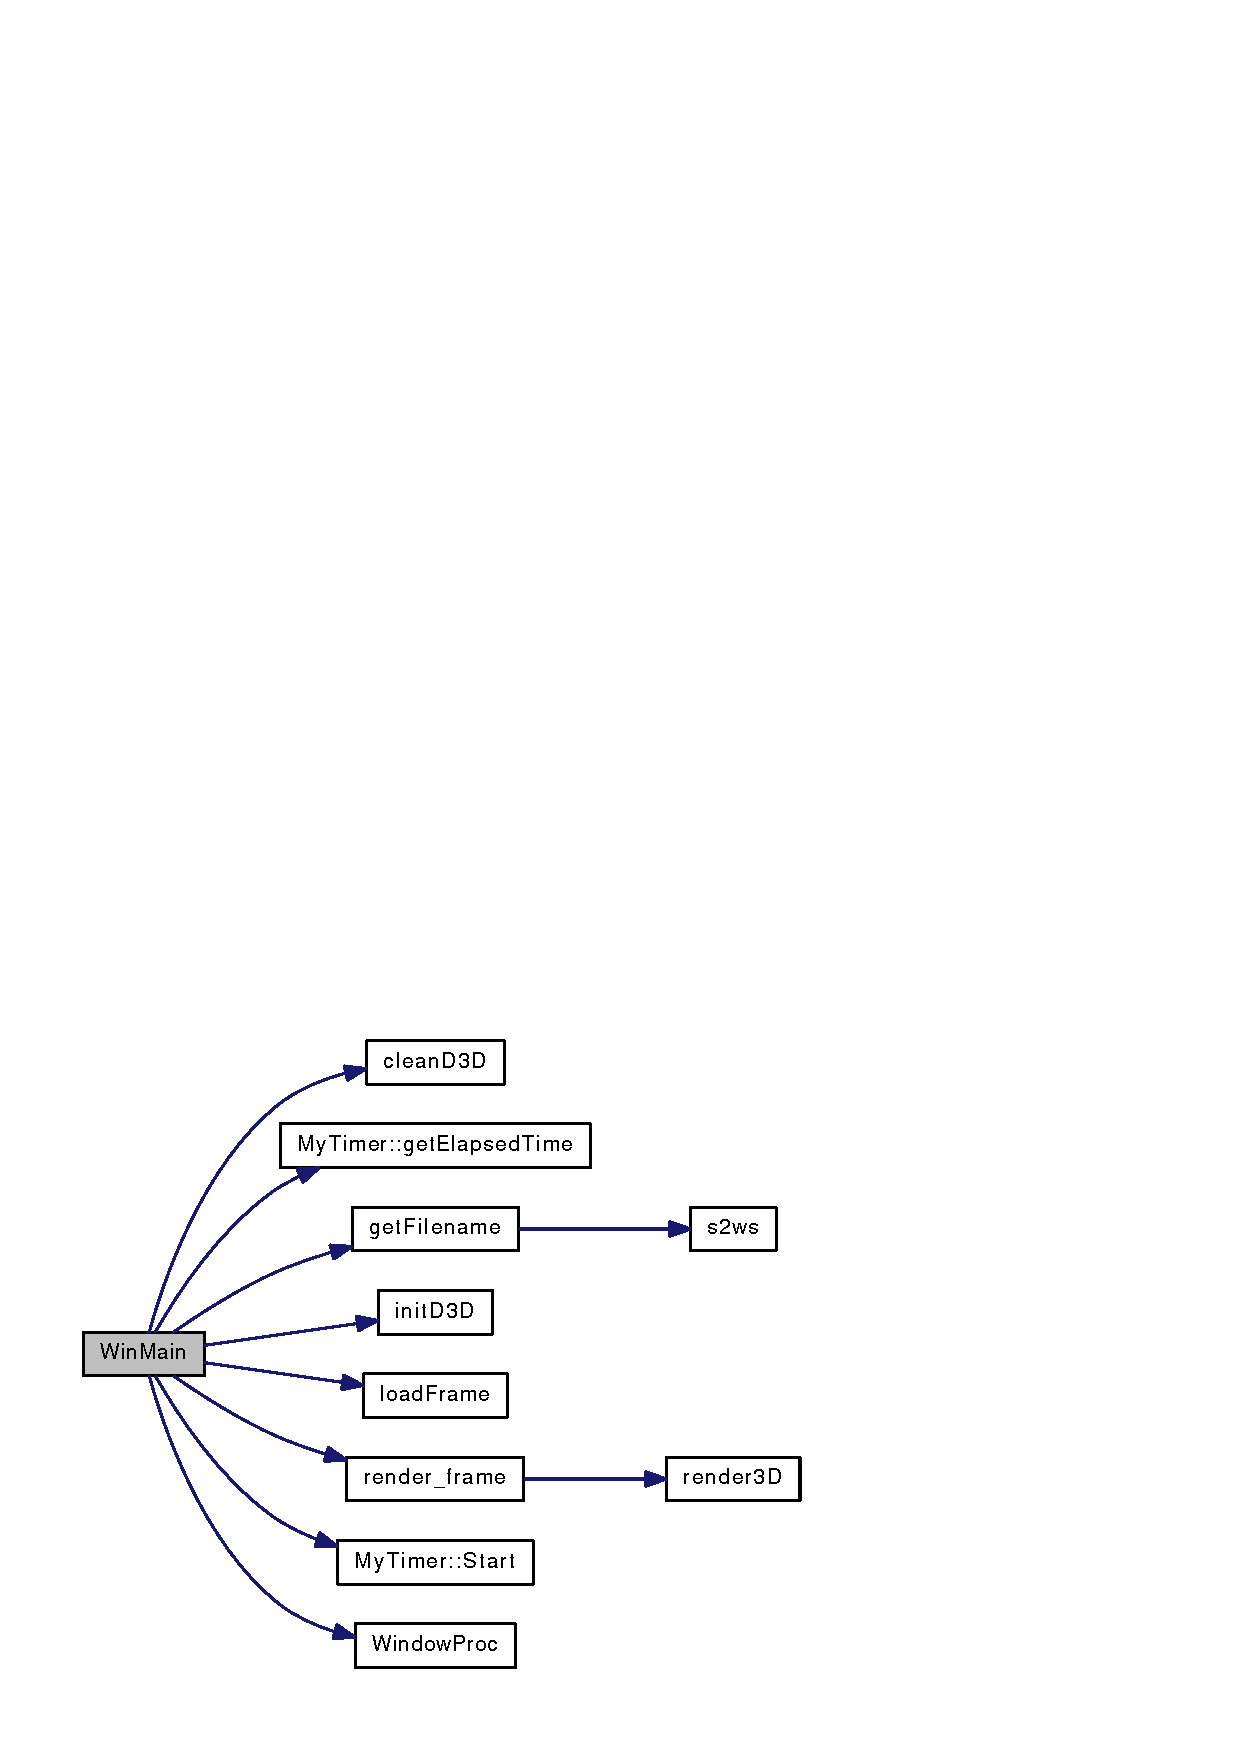
\includegraphics[width=194pt]{main_8cpp_a661c2abc03926acfaeb93b4ae7db4943_cgraph}
\end{center}
\end{figure}




\subsection{Variable Documentation}
\hypertarget{main_8cpp_aa8a3bb0b341846489cc307333d1d9811}{
\index{main.cpp@{main.cpp}!d3d@{d3d}}
\index{d3d@{d3d}!main.cpp@{main.cpp}}
\subsubsection[{d3d}]{\setlength{\rightskip}{0pt plus 5cm}LPDIRECT3D9 {\bf d3d}}}
\label{main_8cpp_aa8a3bb0b341846489cc307333d1d9811}


Definition at line \hyperlink{main_8cpp_source_l00026}{26} of file \hyperlink{main_8cpp_source}{main.cpp}.

\hypertarget{main_8cpp_a1c4528473f1127613d4edcaac0dad7f1}{
\index{main.cpp@{main.cpp}!d3ddev@{d3ddev}}
\index{d3ddev@{d3ddev}!main.cpp@{main.cpp}}
\subsubsection[{d3ddev}]{\setlength{\rightskip}{0pt plus 5cm}LPDIRECT3DDEVICE9 {\bf d3ddev}}}
\label{main_8cpp_a1c4528473f1127613d4edcaac0dad7f1}


Definition at line \hyperlink{main_8cpp_source_l00027}{27} of file \hyperlink{main_8cpp_source}{main.cpp}.

\hypertarget{main_8cpp_a908970643424027cd7df53bf68a9cdad}{
\index{main.cpp@{main.cpp}!destRect@{destRect}}
\index{destRect@{destRect}!main.cpp@{main.cpp}}
\subsubsection[{destRect}]{\setlength{\rightskip}{0pt plus 5cm}RECT {\bf destRect}}}
\label{main_8cpp_a908970643424027cd7df53bf68a9cdad}


Definition at line \hyperlink{main_8cpp_source_l00030}{30} of file \hyperlink{main_8cpp_source}{main.cpp}.

\hypertarget{main_8cpp_a94593fcbf19d34c0830799636182170e}{
\index{main.cpp@{main.cpp}!gBackBuf@{gBackBuf}}
\index{gBackBuf@{gBackBuf}!main.cpp@{main.cpp}}
\subsubsection[{gBackBuf}]{\setlength{\rightskip}{0pt plus 5cm}IDirect3DSurface9$\ast$ {\bf gBackBuf} = NULL}}
\label{main_8cpp_a94593fcbf19d34c0830799636182170e}


Definition at line \hyperlink{main_8cpp_source_l00029}{29} of file \hyperlink{main_8cpp_source}{main.cpp}.

\hypertarget{main_8cpp_a35944f88a0c5556a08bd1da88b8d89db}{
\index{main.cpp@{main.cpp}!gImageSrc@{gImageSrc}}
\index{gImageSrc@{gImageSrc}!main.cpp@{main.cpp}}
\subsubsection[{gImageSrc}]{\setlength{\rightskip}{0pt plus 5cm}IDirect3DSurface9$\ast$ {\bf gImageSrc} = NULL}}
\label{main_8cpp_a35944f88a0c5556a08bd1da88b8d89db}


Definition at line \hyperlink{main_8cpp_source_l00028}{28} of file \hyperlink{main_8cpp_source}{main.cpp}.


\hypertarget{main_8cpp_source}{
\section{/Volumes/BOOTCAMP/Workspace/Solutions/MVC/proj/Direct3DTutorial/Direct3DTutorial/main.cpp}
}


\begin{footnotesize}\begin{alltt}
00001 \textcolor{comment}{// include the basic windows header files and the Direct 3D header file}
00002 \textcolor{preprocessor}{#include <windows.h>}
00003 \textcolor{preprocessor}{#include <windowsx.h>}
00004 \textcolor{preprocessor}{#include <d3d9.h>}
00005 \textcolor{preprocessor}{#include <d3dx9.h>}
00006 
00007 \textcolor{preprocessor}{#include <string>}
00008 \textcolor{preprocessor}{#include <iostream>}
00009 \textcolor{preprocessor}{#include <fstream>}
00010 \textcolor{preprocessor}{#include <sstream>}
00011 \textcolor{preprocessor}{#include <iomanip>}
00012 \textcolor{preprocessor}{#include <cstdlib>}
00013 \textcolor{preprocessor}{#include <atlconv.h>}
00014 
00015 \textcolor{preprocessor}{#include "\hyperlink{mytimer_8h}{mytimer.h}"}
00016 \textcolor{preprocessor}{#include "\hyperlink{utils_8h}{utils.h}"}
00017 \textcolor{preprocessor}{#include "\hyperlink{config_8h}{config.h}"}
00018 
00019 \textcolor{comment}{// include the Direct3D Libary file}
00020 \textcolor{preprocessor}{#pragma comment (lib, "d3d9.lib")}
00021 \textcolor{preprocessor}{}\textcolor{preprocessor}{#pragma comment (lib, "d3dx9.lib")}
00022 \textcolor{preprocessor}{}
00023 \textcolor{keyword}{using namespace }std;
00024 
00025 \textcolor{comment}{// global declarations}
\hypertarget{main_8cpp_source_l00026}{}\hyperlink{main_8cpp_aa8a3bb0b341846489cc307333d1d9811}{00026} LPDIRECT3D9 \hyperlink{main_8cpp_aa8a3bb0b341846489cc307333d1d9811}{d3d};\textcolor{comment}{//pointer to our Direct3D interface}
\hypertarget{main_8cpp_source_l00027}{}\hyperlink{main_8cpp_a1c4528473f1127613d4edcaac0dad7f1}{00027} LPDIRECT3DDEVICE9 \hyperlink{main_8cpp_a1c4528473f1127613d4edcaac0dad7f1}{d3ddev};\textcolor{comment}{// the pointer to the device class}
\hypertarget{main_8cpp_source_l00028}{}\hyperlink{main_8cpp_a35944f88a0c5556a08bd1da88b8d89db}{00028} IDirect3DSurface9*      \hyperlink{main_8cpp_a35944f88a0c5556a08bd1da88b8d89db}{gImageSrc} = NULL; \textcolor{comment}{//Source stereo image}
\hypertarget{main_8cpp_source_l00029}{}\hyperlink{main_8cpp_a94593fcbf19d34c0830799636182170e}{00029} IDirect3DSurface9* \hyperlink{main_8cpp_a94593fcbf19d34c0830799636182170e}{gBackBuf} = NULL;
\hypertarget{main_8cpp_source_l00030}{}\hyperlink{main_8cpp_a908970643424027cd7df53bf68a9cdad}{00030} RECT \hyperlink{main_8cpp_a908970643424027cd7df53bf68a9cdad}{destRect}; \textcolor{comment}{// rectangle to change the destination of the 2 image we are loadi
      ng}
00031 
00032 \textcolor{comment}{//function prototypes}
00033 \textcolor{keywordtype}{void} \hyperlink{main_8cpp_adc57d8d64e4c467f6818cddd81090db7}{initD3D}(HWND hWnd);\textcolor{comment}{// set up and initializes Direct3D}
00034 \textcolor{keywordtype}{void} \hyperlink{main_8cpp_a9d208c9398ed462c31771146011c45a6}{render_frame}(\textcolor{keywordtype}{void});\textcolor{comment}{// renders a single frame}
00035 \textcolor{keywordtype}{void} \hyperlink{main_8cpp_a6e0493c83a486408dbfaae7812e6e47a}{cleanD3D}(\textcolor{keywordtype}{void});\textcolor{comment}{// closes Direct3D and releases memory}
00036 \textcolor{keywordtype}{void} \hyperlink{main_8cpp_a6deb2598e68338891c9b1faadea263b9}{getFilename}(\textcolor{keywordtype}{int}); \textcolor{comment}{// get filename of the next img src}
00037 \textcolor{keywordtype}{void} \hyperlink{main_8cpp_a117a4ee6ce2172cb8d6b4ac48a6c3645}{loadFrame}(\textcolor{keywordtype}{int}); \textcolor{comment}{// load dual-view frames}
00038 \textcolor{keywordtype}{void} \hyperlink{main_8cpp_a94b4e3bf0d4387b63e1bc86968b6550d}{render3D}(\textcolor{keywordtype}{void}); \textcolor{comment}{// stretches our surface to the backbuffer}
00039 
00040 
00041 \textcolor{comment}{// the WindowProc function prototype}
00042 LRESULT CALLBACK \hyperlink{main_8cpp_a3481ed5b54326a7e5b2562195ee71a58}{WindowProc}(HWND hWnd, UINT message,WPARAM wParam,LPARAM lParam);
      
00043 
00044 
00045 \textcolor{comment}{// the entry point for any Windows program}
\hypertarget{main_8cpp_source_l00046}{}\hyperlink{main_8cpp_a661c2abc03926acfaeb93b4ae7db4943}{00046} \textcolor{keywordtype}{int} WINAPI \hyperlink{main_8cpp_a661c2abc03926acfaeb93b4ae7db4943}{WinMain}(HINSTANCE hInstance,HINSTANCE hPrevInstance,LPSTR lpCmdLine,\textcolor{keywordtype}{in
      t} nCmdShow) \{
00047         \textcolor{comment}{// the handle for the window, filled by a function}
00048         HWND hWnd;
00049         \textcolor{comment}{// this struct holds information for the window class}
00050         WNDCLASSEX wc;
00051 
00052         \textcolor{comment}{// clear out the window class for use}
00053         ZeroMemory(&wc, \textcolor{keyword}{sizeof}(WNDCLASSEX));
00054 
00055         \textcolor{comment}{// fill in the struct with the needed information}
00056         wc.cbSize = \textcolor{keyword}{sizeof}(WNDCLASSEX);
00057         wc.style = CS\_HREDRAW | CS\_VREDRAW;
00058         wc.lpfnWndProc = \hyperlink{main_8cpp_a3481ed5b54326a7e5b2562195ee71a58}{WindowProc};
00059         wc.hInstance = hInstance;
00060         wc.hCursor = LoadCursor(NULL, IDC\_ARROW);
00061         \textcolor{comment}{// wc.hbrBackground = (HBRUSH)COLOR\_WINDOW;}
00062         \textcolor{keywordtype}{string} lpszClassNameStr = \textcolor{stringliteral}{"WindowClass1"};
00063         \textcolor{keywordtype}{string} windowNameStr = \textcolor{stringliteral}{"3DVision Test"};
00064         wc.lpszClassName = lpszClassNameStr.c\_str();
00065 
00066         \textcolor{comment}{// register the window class}
00067         RegisterClassEx(&wc);
00068 
00069         \textcolor{comment}{// create the window and use the result as the handle}
00070         hWnd = CreateWindowEx(NULL,
00071                 lpszClassNameStr.c\_str(),\textcolor{comment}{// name of the window class}
00072                 windowNameStr.c\_str(), \textcolor{comment}{// title of the window}
00073                 WS\_EX\_TOPMOST | WS\_POPUP,\textcolor{comment}{// fullscreen values}
00074                 0,\textcolor{comment}{// x-position of the window}
00075                 0,\textcolor{comment}{// y-position of the window}
00076                 \hyperlink{config_8h_a5dde88e08c88df4ec4c201ab068a909b}{gImageWidth},\textcolor{comment}{// width of the window}
00077                 \hyperlink{config_8h_af737c15e6577f2676602957bc1ac2ab1}{gImageHeight},\textcolor{comment}{// height of the window}
00078                 NULL,\textcolor{comment}{// we have no parent window, NULL}
00079                 NULL,\textcolor{comment}{// we aren't using menus, NULL}
00080                 hInstance,\textcolor{comment}{// application handle}
00081                 NULL);\textcolor{comment}{// used with multiple windows, NULL}
00082 
00083         \textcolor{comment}{// display the window on the screen}
00084         ShowWindow(hWnd, nCmdShow);
00085 
00086         \textcolor{comment}{// set up and initialize Direct3D}
00087         \hyperlink{main_8cpp_adc57d8d64e4c467f6818cddd81090db7}{initD3D}(hWnd);
00088 
00089         \textcolor{comment}{//3D VISION}
00090         \textcolor{comment}{// create the surface}
00091         \hyperlink{main_8cpp_a1c4528473f1127613d4edcaac0dad7f1}{d3ddev}->CreateOffscreenPlainSurface(gImageWidth *2, gImageHeight + 1, D3D
      FMT\_A8R8G8B8, D3DPOOL\_DEFAULT, &\hyperlink{main_8cpp_a35944f88a0c5556a08bd1da88b8d89db}{gImageSrc}, NULL);
00092 
00093 
00094         \hyperlink{config_8h_a0a2814a2252fee90794304506ef2e9c0}{fout}.open(\textcolor{stringliteral}{"result.txt"});
00095         \hyperlink{class_my_timer}{MyTimer} timerIns;
00096         timerIns.\hyperlink{class_my_timer_a74b18b409d493579f6b3d0972590a7a6}{Start}();
00097         LONGLONG \_start = timerIns.\hyperlink{class_my_timer_abd0f6728cf64f7b5d81235588bb8e3c2}{getElapsedTime}();
00098         LONGLONG \_current;
00099         \textcolor{keywordtype}{int} frameToRender;
00100         \textcolor{keywordtype}{int} lastRenderedFrame = -1;
00101         \textcolor{keywordtype}{bool} buffered = \textcolor{keyword}{false};
00102         \textcolor{keywordtype}{int} counter = 0;        \textcolor{comment}{// rendered frames counter}
00103         \textcolor{keywordtype}{int} bufcounter = 0;     \textcolor{comment}{// loaded frames counter}
00104 
00105         \textcolor{comment}{// Lock the stereo image}
00106         D3DLOCKED\_RECT lr;
00107         \hyperlink{main_8cpp_a35944f88a0c5556a08bd1da88b8d89db}{gImageSrc}->LockRect(&lr,NULL,0);
00108         \textcolor{comment}{// write stereo signature in the last raw of the stereo image}
00109         \hyperlink{struct___nv___stereo___image___header}{LPNVSTEREOIMAGEHEADER} pSIH = (\hyperlink{struct___nv___stereo___image___header}{LPNVSTEREOIMAGEHEADER})(((\textcolor{keywordtype}{unsigned} \textcolor{keywordtype}{char} *) l
      r.pBits) + (lr.Pitch * (gImageHeight)));
00110 
00111         \textcolor{comment}{// Update the signature header values}
00112         pSIH->\hyperlink{struct___nv___stereo___image___header_aac21b6be816ef3e6b98d1f1183263fd9}{dwSignature} = \hyperlink{utils_8h_a75d1758a6dea9bae825f3253943e334a}{NVSTEREO_IMAGE_SIGNATURE};
00113         pSIH->\hyperlink{struct___nv___stereo___image___header_a9a51ead5061c21601c50b0e1ee2be9a0}{dwBPP} = 32;
00114         \textcolor{comment}{//pSIH->dwFlags = SIH\_SWAP\_EYES; // Src image has left on left and right 
      on right, thats why this flag is not needed.}
00115         pSIH->\hyperlink{struct___nv___stereo___image___header_a495218c0378e538de8c3504daa0a0846}{dwWidth} = gImageWidth*2;
00116         pSIH->\hyperlink{struct___nv___stereo___image___header_a72c1451aca7cb9c87540b647d51b25ad}{dwHeight} = gImageHeight;
00117 
00118         \textcolor{comment}{// Unlock surface}
00119         \hyperlink{main_8cpp_a35944f88a0c5556a08bd1da88b8d89db}{gImageSrc}->UnlockRect();
00120 
00121         \textcolor{comment}{// enter the main loop:}
00122 
00123         \textcolor{comment}{// this struct holds Windows event messages}
00124         MSG msg;
00125 
00126         \textcolor{keywordflow}{while}(TRUE) \{
00127                 \textcolor{comment}{// wait for the next message in the queue, store the result in 'm
      sg'}
00128                 \textcolor{keywordflow}{while}(PeekMessage(&msg, NULL, 0, 0, PM\_REMOVE)) \{
00129                         \textcolor{comment}{// translate keystroke messages into the right format}
00130                         TranslateMessage(&msg);
00131 
00132                         \textcolor{comment}{// send the message to the WindowProc function}
00133                         DispatchMessage(&msg);
00134                 \}
00135 
00136                 \textcolor{comment}{// If the message is WM\_QUIT, exit the while loop}
00137                 \textcolor{keywordflow}{if}(msg.message == WM\_QUIT)
00138                         \textcolor{keywordflow}{break};
00139 
00140                 \_current = timerIns.\hyperlink{class_my_timer_abd0f6728cf64f7b5d81235588bb8e3c2}{getElapsedTime}() - \_start;
00141                 frameToRender = (int)(\_current * \hyperlink{config_8h_a63da2a617b72a1630998a4d8b4d26cd3}{fps} / (\textcolor{keywordtype}{double})1000000);
00142                 \textcolor{comment}{//frameToRender = frameToRender % 3 + 400;}
00143                 \textcolor{comment}{//if (counter>250)}
00144                 \textcolor{comment}{//\{}
00145                 \textcolor{comment}{//      break;}
00146                 \textcolor{comment}{//\}}
00147                 \textcolor{keywordflow}{if}(frameToRender + 1 > \hyperlink{config_8h_a0186bee82f4d469206cfcb18da843a46}{totalFrames}) \{
00148                         \textcolor{comment}{//switch to another demo}
00149                         \textcolor{keywordflow}{if}(\hyperlink{config_8h_a64af52e30206638c00ad08ee8894e3c8}{demo} == 2)\{
00150                                 \hyperlink{config_8h_a6082de4d3555d07a84270f7bacac9a63}{prefixL} = \hyperlink{config_8h_afcc1487cc6eb36a2fc6233b441f2787b}{prefixL3};
00151                                 \hyperlink{config_8h_a939852ed72b1f29dd46c267ba1894687}{prefixR} = \hyperlink{config_8h_ad994e29c70b4b20e5aa11c462d2eaa23}{prefixR3};
00152                                 \hyperlink{config_8h_a0186bee82f4d469206cfcb18da843a46}{totalFrames} = \hyperlink{config_8h_a4058af0c43622045689a17dbf546a095}{totalFrames3};
00153                                 \hyperlink{config_8h_a64af52e30206638c00ad08ee8894e3c8}{demo} = 3;
00154                         \}
00155                         \textcolor{keywordflow}{else} \textcolor{keywordflow}{if}(\hyperlink{config_8h_a64af52e30206638c00ad08ee8894e3c8}{demo} == 3)\{
00156                                 \hyperlink{config_8h_a6082de4d3555d07a84270f7bacac9a63}{prefixL} = \hyperlink{config_8h_a5cfb7ac53a84ac65db638d7926c1216b}{prefixL1};
00157                                 \hyperlink{config_8h_a939852ed72b1f29dd46c267ba1894687}{prefixR} = \hyperlink{config_8h_a0cc8c7e0d207c825f13d92d52480abfc}{prefixR1};
00158                                 \hyperlink{config_8h_a0186bee82f4d469206cfcb18da843a46}{totalFrames} = \hyperlink{config_8h_a1daaec6dd86a744de60951adc0d7491c}{totalFrames1};
00159                                 \hyperlink{config_8h_a64af52e30206638c00ad08ee8894e3c8}{demo} = 1;
00160                         \}
00161                         \textcolor{keywordflow}{else} \textcolor{keywordflow}{if}(\hyperlink{config_8h_a64af52e30206638c00ad08ee8894e3c8}{demo} == 1)\{
00162                                 \hyperlink{config_8h_a6082de4d3555d07a84270f7bacac9a63}{prefixL} = \hyperlink{config_8h_ad2536ccefd202465bc9de3185f689385}{prefixL2};
00163                                 \hyperlink{config_8h_a939852ed72b1f29dd46c267ba1894687}{prefixR} = \hyperlink{config_8h_a655684630849cbc78a1a701627a5be79}{prefixR2};
00164                                 \hyperlink{config_8h_a0186bee82f4d469206cfcb18da843a46}{totalFrames} = \hyperlink{config_8h_a30f8e88254cae72861ca9f1082036f13}{totalFrames2};
00165                                 \hyperlink{config_8h_a64af52e30206638c00ad08ee8894e3c8}{demo} = 2;
00166                         \}
00167                         \_start = timerIns.\hyperlink{class_my_timer_abd0f6728cf64f7b5d81235588bb8e3c2}{getElapsedTime}(); \textcolor{comment}{// start over}
00168                         \textcolor{keywordflow}{continue};
00169                         \textcolor{keywordflow}{break};
00170                 \}
00171                 \textcolor{keywordflow}{if}(buffered==\textcolor{keyword}{false}) \{
00172                         \hyperlink{main_8cpp_a6deb2598e68338891c9b1faadea263b9}{getFilename}(lastRenderedFrame+1);
00173                         \hyperlink{main_8cpp_a117a4ee6ce2172cb8d6b4ac48a6c3645}{loadFrame}(lastRenderedFrame+1);
00174                         \textcolor{comment}{//configureSurface();}
00175                         bufcounter++;
00176                         buffered=\textcolor{keyword}{true};
00177                 \}
00178                 \textcolor{keywordflow}{if}(frameToRender!=lastRenderedFrame) \{
00179                         \textcolor{comment}{//fout<<"rendering frame "<<frameToRender<<endl;}
00180                         \hyperlink{main_8cpp_a9d208c9398ed462c31771146011c45a6}{render_frame}();
00181                         counter++;
00182                         lastRenderedFrame = frameToRender;
00183                         buffered = \textcolor{keyword}{false};
00184                 \}
00185         \}
00186 
00187         \textcolor{comment}{// clean up DirectX and COM}
00188 
00189         \hyperlink{config_8h_a0a2814a2252fee90794304506ef2e9c0}{fout}<< \textcolor{stringliteral}{"total frames buffered = "}<<bufcounter<<endl;
00190         \hyperlink{config_8h_a0a2814a2252fee90794304506ef2e9c0}{fout}<< \textcolor{stringliteral}{"total frames rendered = "}<<counter<<endl;
00191         \textcolor{keywordtype}{double} perf = (double)counter * 1000000/ timerIns.\hyperlink{class_my_timer_abd0f6728cf64f7b5d81235588bb8e3c2}{getElapsedTime}();
00192         \hyperlink{config_8h_a0a2814a2252fee90794304506ef2e9c0}{fout} << \textcolor{stringliteral}{"actual fps reached = "}<< perf << endl;
00193         \hyperlink{config_8h_a0a2814a2252fee90794304506ef2e9c0}{fout}.close();
00194         \textcolor{comment}{// return this part of the WM\_QUIT message to Windows}
00195         \hyperlink{main_8cpp_a6e0493c83a486408dbfaae7812e6e47a}{cleanD3D}();
00196         \textcolor{keywordflow}{return} msg.wParam;
00197 \}
00198 
00200 \textcolor{comment}{// this is the main message handler for the program}
\hypertarget{main_8cpp_source_l00201}{}\hyperlink{main_8cpp_a3481ed5b54326a7e5b2562195ee71a58}{00201} LRESULT CALLBACK \hyperlink{main_8cpp_a3481ed5b54326a7e5b2562195ee71a58}{WindowProc}(HWND hWnd, UINT message, WPARAM wParam, LPARAM lParam
      ) \{
00202         \textcolor{comment}{// sort through and find what code to run for the message given}
00203         \textcolor{keywordflow}{switch}(message) \{
00204                 \textcolor{comment}{// this message is read when the window is closed}
00205 \textcolor{keywordflow}{case} WM\_DESTROY: \{
00206         \textcolor{comment}{// close the application entirely}
00207         PostQuitMessage(0);
00208         \textcolor{keywordflow}{return} 0;
00209                                  \}
00210                                  \textcolor{keywordflow}{break};
00211         \}
00212 
00213         \textcolor{comment}{// Handle any messages the switch statement didn't}
00214         \textcolor{keywordflow}{return} DefWindowProc (hWnd, message, wParam, lParam);
00215 \}
00216 
00217 \textcolor{comment}{// this function initializes and prepares Direct3D for use}
\hypertarget{main_8cpp_source_l00218}{}\hyperlink{main_8cpp_adc57d8d64e4c467f6818cddd81090db7}{00218} \textcolor{keywordtype}{void} \hyperlink{main_8cpp_adc57d8d64e4c467f6818cddd81090db7}{initD3D}(HWND hWnd) \{
00219         \hyperlink{main_8cpp_aa8a3bb0b341846489cc307333d1d9811}{d3d} = Direct3DCreate9(D3D\_SDK\_VERSION);\textcolor{comment}{// create the Direct3D interface}
00220 
00221         D3DPRESENT\_PARAMETERS d3dpp;\textcolor{comment}{// create a struct to hold various device inf
      ormation}
00222 
00223         ZeroMemory(&d3dpp, \textcolor{keyword}{sizeof}(d3dpp));\textcolor{comment}{// clear out the struct for use}
00224         d3dpp.Windowed = FALSE;\textcolor{comment}{// program fullscreen}
00225         d3dpp.SwapEffect = D3DSWAPEFFECT\_DISCARD;\textcolor{comment}{// discard old frames}
00226         d3dpp.hDeviceWindow = hWnd;\textcolor{comment}{// set the window to be used by Direct3D}
00227         d3dpp.BackBufferFormat = D3DFMT\_A8R8G8B8;\textcolor{comment}{// set the back buffer format to
       32 bit}
00228         d3dpp.BackBufferWidth = \hyperlink{config_8h_a5dde88e08c88df4ec4c201ab068a909b}{gImageWidth};
00229         d3dpp.BackBufferHeight = \hyperlink{config_8h_af737c15e6577f2676602957bc1ac2ab1}{gImageHeight};
00230         d3dpp.PresentationInterval = D3DPRESENT\_INTERVAL\_ONE;
00231         d3dpp.BackBufferCount = 1;
00232 
00233         \textcolor{comment}{// create a device class using this information and information from the 
      d3dpp struct}
00234         \hyperlink{main_8cpp_aa8a3bb0b341846489cc307333d1d9811}{d3d}->CreateDevice(D3DADAPTER\_DEFAULT,D3DDEVTYPE\_HAL,hWnd,D3DCREATE\_SOFTWA
      RE\_VERTEXPROCESSING,&d3dpp,&\hyperlink{main_8cpp_a1c4528473f1127613d4edcaac0dad7f1}{d3ddev});
00235 \}
00236 
00237 \textcolor{comment}{// this is the function used to render a single frame}
\hypertarget{main_8cpp_source_l00238}{}\hyperlink{main_8cpp_a9d208c9398ed462c31771146011c45a6}{00238} \textcolor{keywordtype}{void} \hyperlink{main_8cpp_a9d208c9398ed462c31771146011c45a6}{render_frame}(\textcolor{keywordtype}{void}) \{
00239         \textcolor{comment}{// clear the window to a deep blue}
00240         \hyperlink{main_8cpp_a1c4528473f1127613d4edcaac0dad7f1}{d3ddev}->Clear(0, NULL, D3DCLEAR\_TARGET, D3DCOLOR\_XRGB(0, 40, 100), 1.0f, 
      0);
00241 
00242         \hyperlink{main_8cpp_a1c4528473f1127613d4edcaac0dad7f1}{d3ddev}->BeginScene();\textcolor{comment}{// begins the 3D scene}
00243 
00244         \textcolor{comment}{// do 3D rendering on the back buffer here}
00245         \hyperlink{main_8cpp_a94b4e3bf0d4387b63e1bc86968b6550d}{render3D}();
00246 
00247 
00248         \hyperlink{main_8cpp_a1c4528473f1127613d4edcaac0dad7f1}{d3ddev}->EndScene();\textcolor{comment}{// ends the 3D scene}
00249 
00250         \hyperlink{main_8cpp_a1c4528473f1127613d4edcaac0dad7f1}{d3ddev}->Present(NULL, NULL, NULL, NULL);\textcolor{comment}{// displays the created frame}
00251 \}
00252 
00253 
00254 \textcolor{comment}{// this is the function that cleans up Direct3D and COM}
\hypertarget{main_8cpp_source_l00255}{}\hyperlink{main_8cpp_a6e0493c83a486408dbfaae7812e6e47a}{00255} \textcolor{keywordtype}{void} \hyperlink{main_8cpp_a6e0493c83a486408dbfaae7812e6e47a}{cleanD3D}(\textcolor{keywordtype}{void}) \{
00256         \hyperlink{main_8cpp_a1c4528473f1127613d4edcaac0dad7f1}{d3ddev}->Release();\textcolor{comment}{// close and release the 3D device}
00257         \hyperlink{main_8cpp_aa8a3bb0b341846489cc307333d1d9811}{d3d}->Release();\textcolor{comment}{// close and release Direct3D}
00258 \}
00259 
00260 
00261 \textcolor{comment}{// this is the function that combines two images.}
\hypertarget{main_8cpp_source_l00262}{}\hyperlink{main_8cpp_a94b4e3bf0d4387b63e1bc86968b6550d}{00262} \textcolor{keywordtype}{void} \hyperlink{main_8cpp_a94b4e3bf0d4387b63e1bc86968b6550d}{render3D}(\textcolor{keywordtype}{void}) \{
00263         \textcolor{comment}{// set destRect}
00264         \hyperlink{main_8cpp_a908970643424027cd7df53bf68a9cdad}{destRect}.left = 0;
00265         \hyperlink{main_8cpp_a908970643424027cd7df53bf68a9cdad}{destRect}.top = 0;
00266         \hyperlink{main_8cpp_a908970643424027cd7df53bf68a9cdad}{destRect}.bottom = \hyperlink{config_8h_af737c15e6577f2676602957bc1ac2ab1}{gImageHeight};
00267         \hyperlink{main_8cpp_a908970643424027cd7df53bf68a9cdad}{destRect}.right = \hyperlink{config_8h_a5dde88e08c88df4ec4c201ab068a909b}{gImageWidth};
00268 
00269         \textcolor{comment}{// Get the Backbuffer then Stretch the Surface on it.}
00270         \hyperlink{main_8cpp_a1c4528473f1127613d4edcaac0dad7f1}{d3ddev}->GetBackBuffer(0, 0, D3DBACKBUFFER\_TYPE\_MONO, &\hyperlink{main_8cpp_a94593fcbf19d34c0830799636182170e}{gBackBuf});
00271         \hyperlink{main_8cpp_a1c4528473f1127613d4edcaac0dad7f1}{d3ddev}->StretchRect(\hyperlink{main_8cpp_a35944f88a0c5556a08bd1da88b8d89db}{gImageSrc}, NULL, \hyperlink{main_8cpp_a94593fcbf19d34c0830799636182170e}{gBackBuf}, &\hyperlink{main_8cpp_a908970643424027cd7df53bf68a9cdad}{destRect}, D3DTEXF\_NONE);
00272 \}
00273 
\hypertarget{main_8cpp_source_l00274}{}\hyperlink{main_8cpp_aad6fe44abbb9cde538b5e84718ee3526}{00274} wstring \hyperlink{main_8cpp_aad6fe44abbb9cde538b5e84718ee3526}{s2ws}(\textcolor{keyword}{const} \textcolor{keywordtype}{string}& s) \{
00275         \textcolor{keywordtype}{int} len;
00276         \textcolor{keywordtype}{int} slength = (int)s.length() + 1;
00277         len = MultiByteToWideChar(CP\_ACP, 0, s.c\_str(), slength, 0, 0);
00278         \textcolor{keywordtype}{wchar\_t}* buf = \textcolor{keyword}{new} \textcolor{keywordtype}{wchar\_t}[len];
00279         MultiByteToWideChar(CP\_ACP, 0, s.c\_str(), slength, buf, len);
00280         wstring r(buf);
00281         \textcolor{keyword}{delete}[] buf;
00282         \textcolor{keywordflow}{return} r;
00283 \}
00284 
\hypertarget{main_8cpp_source_l00285}{}\hyperlink{main_8cpp_a6deb2598e68338891c9b1faadea263b9}{00285} \textcolor{keywordtype}{void} \hyperlink{main_8cpp_a6deb2598e68338891c9b1faadea263b9}{getFilename}(\textcolor{keywordtype}{int} \_frame) \{
00286         stringstream filenamer;
00287 
00288         filenamer<<\hyperlink{config_8h_a6082de4d3555d07a84270f7bacac9a63}{prefixL}<<setw(4)<<setfill(\textcolor{charliteral}{'0'})<<\_frame<<\hyperlink{config_8h_a887452eecbb8843e5530a1597eb8e357}{suffix};
00289         \textcolor{comment}{//filenamer<<prefixL<<\_frame<<suffix;}
00290         filenamer>>\hyperlink{config_8h_a65980faa7a98d89e3581eb3ac8777192}{filenameStrL};
00291         \hyperlink{config_8h_a526270325c61739d50933ee42ef9563f}{filenameWstrL} = \hyperlink{main_8cpp_aad6fe44abbb9cde538b5e84718ee3526}{s2ws}(filenameStrL);
00292 
00293         filenamer.clear();
00294         filenamer<<\hyperlink{config_8h_a939852ed72b1f29dd46c267ba1894687}{prefixR}<<setw(4)<<setfill(\textcolor{charliteral}{'0'})<<\_frame<<suffix;
00295         \textcolor{comment}{//filenamer<<prefixR<<\_frame<<suffix;}
00296         filenamer>>\hyperlink{config_8h_a19fa526345d6a5020afd0ef78ab58f71}{filenameStrR};
00297         filenamer.clear();
00298         \hyperlink{config_8h_a3b06e388f8261198f0fe86aafca02c41}{filenameWstrR} = \hyperlink{main_8cpp_aad6fe44abbb9cde538b5e84718ee3526}{s2ws}(filenameStrR);
00299 
00300         \hyperlink{config_8h_a9e78e5f975acc8e56d6a84214321a534}{filenameL} = \hyperlink{config_8h_a526270325c61739d50933ee42ef9563f}{filenameWstrL}.c\_str();
00301         \hyperlink{config_8h_ab2d091b589f33f799378b4dbf379e537}{filenameR} = \hyperlink{config_8h_a3b06e388f8261198f0fe86aafca02c41}{filenameWstrR}.c\_str();
00302         \hyperlink{config_8h_a4efd8a98fc24b184ad75501454b3c2b7}{filenameLL} = filenameStrL.c\_str();
00303         \hyperlink{config_8h_ac31be6060769b3c9c0c533e0cf269b28}{filenameRR} = filenameStrR.c\_str();
00304 \}
00305 
\hypertarget{main_8cpp_source_l00306}{}\hyperlink{main_8cpp_a117a4ee6ce2172cb8d6b4ac48a6c3645}{00306} \textcolor{keywordtype}{void} \hyperlink{main_8cpp_a117a4ee6ce2172cb8d6b4ac48a6c3645}{loadFrame}(\textcolor{keywordtype}{int} \_frame) \{
00307         \textcolor{keyword}{static} \textcolor{keywordtype}{bool} loaded = \textcolor{keyword}{false};
00308         \textcolor{keyword}{static} \textcolor{keywordtype}{char} *data1 = 0, *data2 = 0;
00309         \textcolor{keywordtype}{int} dataSize1 = 0, dataSize2 = 0;
00310         \textcolor{comment}{/*}
00311 \textcolor{comment}{        // set up destRect}
00312 \textcolor{comment}{        destRect.left = 0;}
00313 \textcolor{comment}{        destRect.top = 0;}
00314 \textcolor{comment}{        destRect.bottom = gImageHeight;}
00315 \textcolor{comment}{        destRect.right = gImageWidth;}
00316 \textcolor{comment}{        //if (!loaded)}
00317 \textcolor{comment}{        \{}
00318 \textcolor{comment}{        loaded = true;}
00319 \textcolor{comment}{        fout << "load file\(\backslash\)n";}
00320 \textcolor{comment}{        FILE *f = fopen(filenameStrL.c\_str(), "rb");}
00321 \textcolor{comment}{        //fseek(f, 0, SEEK\_END);}
00322 \textcolor{comment}{        //int fsize = ftell(f);}
00323 \textcolor{comment}{        //fseek(f, 0, SEEK\_SET);}
00324 \textcolor{comment}{        fout << "file loaded \(\backslash\)n";}
00325 \textcolor{comment}{        int fsize = 10 * 1024 * 1024;}
00326 \textcolor{comment}{        data1 = new char[10*1024*1024];}
00327 \textcolor{comment}{        dataSize1 = fread(data1, 1, fsize, f);}
00328 \textcolor{comment}{        fclose(f);}
00329 \textcolor{comment}{}
00330 \textcolor{comment}{        f = fopen(filenameStrR.c\_str(), "rb");}
00331 \textcolor{comment}{        //fseek(f, 0, SEEK\_END);}
00332 \textcolor{comment}{        //fsize = ftell(f);}
00333 \textcolor{comment}{        //fseek(f, 0, SEEK\_SET);}
00334 \textcolor{comment}{        data2 = new char[fsize];}
00335 \textcolor{comment}{        dataSize2 = fread(data2, 1, fsize, f);}
00336 \textcolor{comment}{        fclose(f);}
00337 \textcolor{comment}{}
00338 \textcolor{comment}{        fout << "Size = " << dataSize1 << " " << dataSize2 << endl;}
00339 \textcolor{comment}{        \}}
00340 \textcolor{comment}{}
00341 \textcolor{comment}{        D3DXLoadSurfaceFromMemory(gImageSrc, NULL, &destRect, data1, D3DFMT\_A8R8G
      8B8, 0, NULL, NULL,D3DX\_DEFAULT, 0);}
00342 \textcolor{comment}{        destRect.left = gImageWidth;}
00343 \textcolor{comment}{        destRect.top = 0;}
00344 \textcolor{comment}{        destRect.bottom = gImageHeight;}
00345 \textcolor{comment}{        destRect.right = gImageWidth*2;}
00346 \textcolor{comment}{        D3DXLoadSurfaceFromMemory(gImageSrc, NULL, &destRect, data2, D3DFMT\_A8R8G
      8B8, 0, NULL, NULL, D3DX\_DEFAULT, 0);}
00347 \textcolor{comment}{        */}
00348 
00350         \textcolor{comment}{// set up destRect}
00351         \hyperlink{main_8cpp_a908970643424027cd7df53bf68a9cdad}{destRect}.left = 0;
00352         \hyperlink{main_8cpp_a908970643424027cd7df53bf68a9cdad}{destRect}.top = 0;
00353         \hyperlink{main_8cpp_a908970643424027cd7df53bf68a9cdad}{destRect}.bottom = \hyperlink{config_8h_af737c15e6577f2676602957bc1ac2ab1}{gImageHeight};
00354         \hyperlink{main_8cpp_a908970643424027cd7df53bf68a9cdad}{destRect}.right = \hyperlink{config_8h_a5dde88e08c88df4ec4c201ab068a909b}{gImageWidth};
00355 
00356         \textcolor{comment}{// load left image}
00357         D3DXLoadSurfaceFromFile(\hyperlink{main_8cpp_a35944f88a0c5556a08bd1da88b8d89db}{gImageSrc}, NULL, &\hyperlink{main_8cpp_a908970643424027cd7df53bf68a9cdad}{destRect}, \hyperlink{config_8h_a4efd8a98fc24b184ad75501454b3c2b7}{filenameLL}, NULL, D3D
      X\_DEFAULT, 0, NULL);
00358 
00359         \textcolor{comment}{// shift destRect to the right}
00360         \hyperlink{main_8cpp_a908970643424027cd7df53bf68a9cdad}{destRect}.left = \hyperlink{config_8h_a5dde88e08c88df4ec4c201ab068a909b}{gImageWidth};
00361         \hyperlink{main_8cpp_a908970643424027cd7df53bf68a9cdad}{destRect}.top = 0;
00362         \hyperlink{main_8cpp_a908970643424027cd7df53bf68a9cdad}{destRect}.bottom = \hyperlink{config_8h_af737c15e6577f2676602957bc1ac2ab1}{gImageHeight};
00363         \hyperlink{main_8cpp_a908970643424027cd7df53bf68a9cdad}{destRect}.right = \hyperlink{config_8h_a5dde88e08c88df4ec4c201ab068a909b}{gImageWidth}*2;
00364 
00365         \textcolor{comment}{// load right image}
00366         D3DXLoadSurfaceFromFile(\hyperlink{main_8cpp_a35944f88a0c5556a08bd1da88b8d89db}{gImageSrc}, NULL, &\hyperlink{main_8cpp_a908970643424027cd7df53bf68a9cdad}{destRect}, \hyperlink{config_8h_ac31be6060769b3c9c0c533e0cf269b28}{filenameRR}, NULL, D3D
      X\_DEFAULT, 0, NULL);
00367         \textcolor{comment}{//*/}
00368 \}
\end{alltt}\end{footnotesize}

\hypertarget{mytimer_8h}{
\section{/Volumes/BOOTCAMP/Workspace/Solutions/MVC/proj/Direct3DTutorial/Direct3DTutorial/mytimer.h File Reference}
\label{mytimer_8h}\index{/Volumes/BOOTCAMP/Workspace/Solutions/MVC/proj/Direct3DTutorial/Direct3DTutorial/mytimer.h@{/Volumes/BOOTCAMP/Workspace/Solutions/MVC/proj/Direct3DTutorial/Direct3DTutorial/mytimer.h}}
}
{\ttfamily \#include $<$windows.h$>$}\par
Include dependency graph for mytimer.h:\nopagebreak
\begin{figure}[H]
\begin{center}
\leavevmode
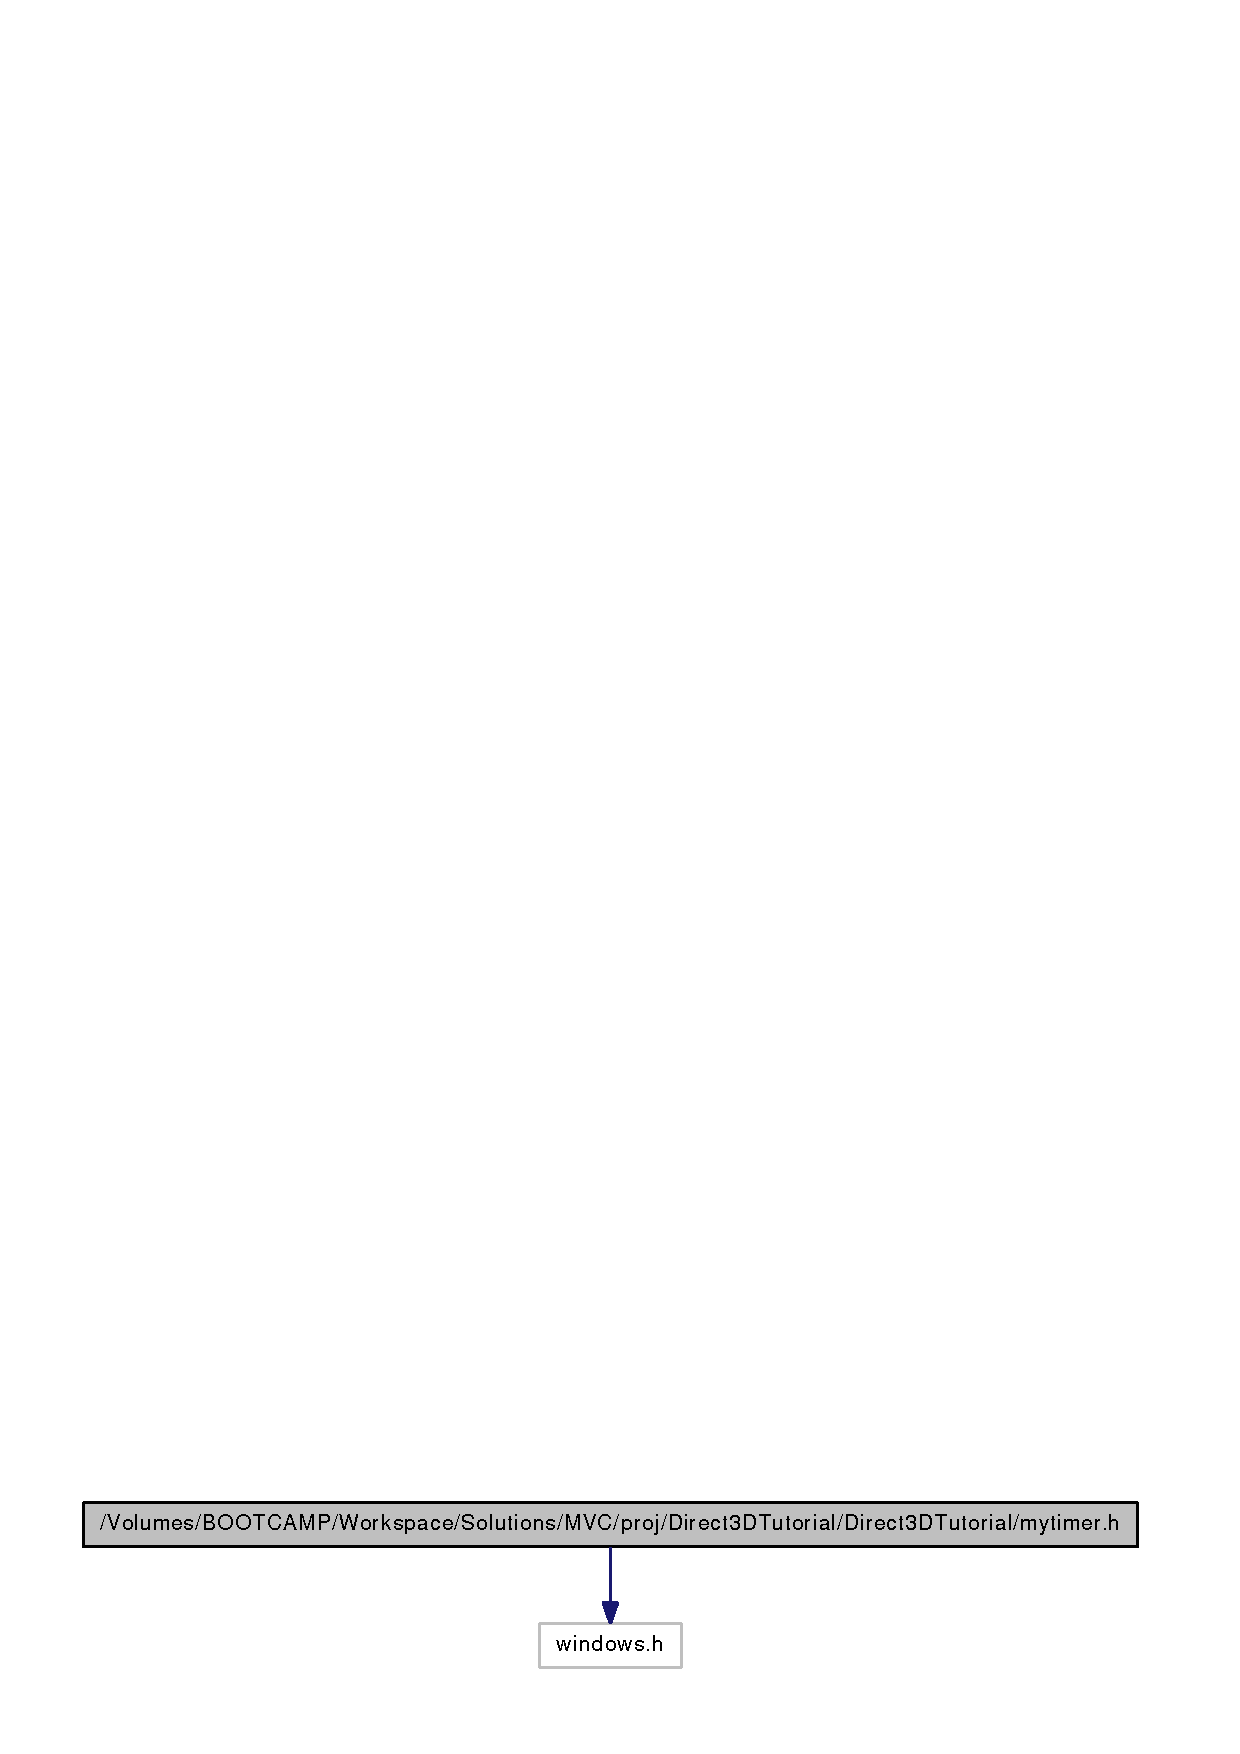
\includegraphics[width=275pt]{mytimer_8h__incl}
\end{center}
\end{figure}
\subsection*{Classes}
\begin{DoxyCompactItemize}
\item 
class \hyperlink{class_my_timer}{MyTimer}
\end{DoxyCompactItemize}

\hypertarget{mytimer_8h_source}{
\section{/Volumes/BOOTCAMP/Workspace/Solutions/MVC/proj/Direct3DTutorial/Direct3DTutorial/mytimer.h}
}


\begin{footnotesize}\begin{alltt}
00001 \textcolor{preprocessor}{#ifndef \_MYTIMER\_H\_}
00002 \textcolor{preprocessor}{}\textcolor{preprocessor}{#define \_MYTIMER\_H\_}
00003 \textcolor{preprocessor}{}\textcolor{preprocessor}{#include <windows.h>}
00004 
\hypertarget{mytimer_8h_source_l00005}{}\hyperlink{class_my_timer}{00005} \textcolor{keyword}{class }\hyperlink{class_my_timer}{MyTimer} \{
00006 \textcolor{keyword}{private}:
00007     LONGLONG \_freq;
00008     LARGE\_INTEGER \_begin;
00009     LARGE\_INTEGER \_current;
00010     LARGE\_INTEGER \_end;
00011 
00012 \textcolor{keyword}{public}:
\hypertarget{mytimer_8h_source_l00013}{}\hyperlink{class_my_timer_adef1d73f6cbdc533c45766b6fa739154}{00013}     LONGLONG \hyperlink{class_my_timer_adef1d73f6cbdc533c45766b6fa739154}{costTime};            \textcolor{comment}{// ���ѵ�ʱ��(��ȷ��ms)}
00014 
00015 \textcolor{keyword}{public}:
\hypertarget{mytimer_8h_source_l00016}{}\hyperlink{class_my_timer_a75440365bcfd96d34be38d8a0c9c014b}{00016}     \hyperlink{class_my_timer_a75440365bcfd96d34be38d8a0c9c014b}{MyTimer}() \{
00017         LARGE\_INTEGER tmp;
00018         QueryPerformanceFrequency(&tmp);
00019         \_freq = tmp.QuadPart;
00020         \hyperlink{class_my_timer_adef1d73f6cbdc533c45766b6fa739154}{costTime} = 0;
00021     \}
00022 
\hypertarget{mytimer_8h_source_l00023}{}\hyperlink{class_my_timer_a74b18b409d493579f6b3d0972590a7a6}{00023}     \textcolor{keywordtype}{void} \hyperlink{class_my_timer_a74b18b409d493579f6b3d0972590a7a6}{Start}() \{
00024         QueryPerformanceCounter(&\_begin);
00025     \}
00026 
\hypertarget{mytimer_8h_source_l00027}{}\hyperlink{class_my_timer_a9c499fe726dbd8a30c528727f42e993d}{00027}     \textcolor{keywordtype}{void} \hyperlink{class_my_timer_a9c499fe726dbd8a30c528727f42e993d}{End}() \{
00028         QueryPerformanceCounter(&\_end);
00029         \hyperlink{class_my_timer_adef1d73f6cbdc533c45766b6fa739154}{costTime} = (LONGLONG)((\_end.QuadPart - \_begin.QuadPart) * 1000000 / \_freq
      );
00030     \}
00031 
\hypertarget{mytimer_8h_source_l00032}{}\hyperlink{class_my_timer_abd0f6728cf64f7b5d81235588bb8e3c2}{00032}     LONGLONG \hyperlink{class_my_timer_abd0f6728cf64f7b5d81235588bb8e3c2}{getElapsedTime}() \{
00033         QueryPerformanceCounter(&\_current);
00034         \textcolor{keywordflow}{return} (LONGLONG)((\_current.QuadPart * 1000000 - \_begin.QuadPart* 1000000
      )  / \_freq);
00035     \}
00036 
\hypertarget{mytimer_8h_source_l00037}{}\hyperlink{class_my_timer_ae616c920850e8d388f93f0d354b25ba5}{00037}     \textcolor{keywordtype}{void} \hyperlink{class_my_timer_ae616c920850e8d388f93f0d354b25ba5}{Reset}() \{
00038         \hyperlink{class_my_timer_adef1d73f6cbdc533c45766b6fa739154}{costTime} = 0;
00039     \}
00040 
\hypertarget{mytimer_8h_source_l00041}{}\hyperlink{class_my_timer_ae695b0dd5d9c28c1d3dc46ba4c616eec}{00041}     \textcolor{keyword}{inline} \textcolor{keywordtype}{unsigned} \_\_int64 \hyperlink{class_my_timer_ae695b0dd5d9c28c1d3dc46ba4c616eec}{GetCycleCount}() \{
00042         \_\_asm \_emit 0x0F
00043         \_\_asm \_emit 0x31
00044     \}
00045 \};
00046 \textcolor{preprocessor}{#endif}
\end{alltt}\end{footnotesize}

\hypertarget{utils_8h}{
\section{/Volumes/BOOTCAMP/Workspace/Solutions/MVC/proj/Direct3DTutorial/Direct3DTutorial/utils.h File Reference}
\label{utils_8h}\index{/Volumes/BOOTCAMP/Workspace/Solutions/MVC/proj/Direct3DTutorial/Direct3DTutorial/utils.h@{/Volumes/BOOTCAMP/Workspace/Solutions/MVC/proj/Direct3DTutorial/Direct3DTutorial/utils.h}}
}
\subsection*{Classes}
\begin{DoxyCompactItemize}
\item 
struct \hyperlink{struct___nv___stereo___image___header}{\_\-Nv\_\-Stereo\_\-Image\_\-Header}
\end{DoxyCompactItemize}
\subsection*{Defines}
\begin{DoxyCompactItemize}
\item 
\#define \hyperlink{utils_8h_a75d1758a6dea9bae825f3253943e334a}{NVSTEREO\_\-IMAGE\_\-SIGNATURE}~0x4433564e
\item 
\#define \hyperlink{utils_8h_a6d44bc2736224ee0c6a2a2993ff68fe4}{SIH\_\-SWAP\_\-EYES}~0x00000001
\item 
\#define \hyperlink{utils_8h_a6783bfb43af2b326cdf8ca43ffa47b5a}{SIH\_\-SCALE\_\-TO\_\-FIT}~0x00000002
\end{DoxyCompactItemize}
\subsection*{Typedefs}
\begin{DoxyCompactItemize}
\item 
typedef struct \hyperlink{struct___nv___stereo___image___header}{\_\-Nv\_\-Stereo\_\-Image\_\-Header} \hyperlink{utils_8h_abb939508f3472b819dc3970388873cd4}{NVSTEREOIMAGEHEADER}
\item 
typedef struct \hyperlink{struct___nv___stereo___image___header}{\_\-Nv\_\-Stereo\_\-Image\_\-Header} $\ast$ \hyperlink{utils_8h_ab31f02c284aafa2623be9cd843915844}{LPNVSTEREOIMAGEHEADER}
\end{DoxyCompactItemize}


\subsection{Define Documentation}
\hypertarget{utils_8h_a75d1758a6dea9bae825f3253943e334a}{
\index{utils.h@{utils.h}!NVSTEREO\_\-IMAGE\_\-SIGNATURE@{NVSTEREO\_\-IMAGE\_\-SIGNATURE}}
\index{NVSTEREO\_\-IMAGE\_\-SIGNATURE@{NVSTEREO\_\-IMAGE\_\-SIGNATURE}!utils.h@{utils.h}}
\subsubsection[{NVSTEREO\_\-IMAGE\_\-SIGNATURE}]{\setlength{\rightskip}{0pt plus 5cm}\#define NVSTEREO\_\-IMAGE\_\-SIGNATURE~0x4433564e}}
\label{utils_8h_a75d1758a6dea9bae825f3253943e334a}


Definition at line \hyperlink{utils_8h_source_l00004}{4} of file \hyperlink{utils_8h_source}{utils.h}.

\hypertarget{utils_8h_a6783bfb43af2b326cdf8ca43ffa47b5a}{
\index{utils.h@{utils.h}!SIH\_\-SCALE\_\-TO\_\-FIT@{SIH\_\-SCALE\_\-TO\_\-FIT}}
\index{SIH\_\-SCALE\_\-TO\_\-FIT@{SIH\_\-SCALE\_\-TO\_\-FIT}!utils.h@{utils.h}}
\subsubsection[{SIH\_\-SCALE\_\-TO\_\-FIT}]{\setlength{\rightskip}{0pt plus 5cm}\#define SIH\_\-SCALE\_\-TO\_\-FIT~0x00000002}}
\label{utils_8h_a6783bfb43af2b326cdf8ca43ffa47b5a}


Definition at line \hyperlink{utils_8h_source_l00018}{18} of file \hyperlink{utils_8h_source}{utils.h}.

\hypertarget{utils_8h_a6d44bc2736224ee0c6a2a2993ff68fe4}{
\index{utils.h@{utils.h}!SIH\_\-SWAP\_\-EYES@{SIH\_\-SWAP\_\-EYES}}
\index{SIH\_\-SWAP\_\-EYES@{SIH\_\-SWAP\_\-EYES}!utils.h@{utils.h}}
\subsubsection[{SIH\_\-SWAP\_\-EYES}]{\setlength{\rightskip}{0pt plus 5cm}\#define SIH\_\-SWAP\_\-EYES~0x00000001}}
\label{utils_8h_a6d44bc2736224ee0c6a2a2993ff68fe4}


Definition at line \hyperlink{utils_8h_source_l00017}{17} of file \hyperlink{utils_8h_source}{utils.h}.



\subsection{Typedef Documentation}
\hypertarget{utils_8h_ab31f02c284aafa2623be9cd843915844}{
\index{utils.h@{utils.h}!LPNVSTEREOIMAGEHEADER@{LPNVSTEREOIMAGEHEADER}}
\index{LPNVSTEREOIMAGEHEADER@{LPNVSTEREOIMAGEHEADER}!utils.h@{utils.h}}
\subsubsection[{LPNVSTEREOIMAGEHEADER}]{\setlength{\rightskip}{0pt plus 5cm}typedef struct {\bf \_\-Nv\_\-Stereo\_\-Image\_\-Header} $\ast$ {\bf LPNVSTEREOIMAGEHEADER}}}
\label{utils_8h_ab31f02c284aafa2623be9cd843915844}
\hypertarget{utils_8h_abb939508f3472b819dc3970388873cd4}{
\index{utils.h@{utils.h}!NVSTEREOIMAGEHEADER@{NVSTEREOIMAGEHEADER}}
\index{NVSTEREOIMAGEHEADER@{NVSTEREOIMAGEHEADER}!utils.h@{utils.h}}
\subsubsection[{NVSTEREOIMAGEHEADER}]{\setlength{\rightskip}{0pt plus 5cm}typedef struct {\bf \_\-Nv\_\-Stereo\_\-Image\_\-Header}  {\bf NVSTEREOIMAGEHEADER}}}
\label{utils_8h_abb939508f3472b819dc3970388873cd4}

\hypertarget{utils_8h_source}{
\section{/Volumes/BOOTCAMP/Workspace/Solutions/MVC/proj/Direct3DTutorial/Direct3DTutorial/utils.h}
}


\begin{footnotesize}\begin{alltt}
00001 \textcolor{comment}{// Nvidia Stereo signature}
00002 
00003 \textcolor{comment}{// Stereo Blitdefines}
\hypertarget{utils_8h_source_l00004}{}\hyperlink{utils_8h_a75d1758a6dea9bae825f3253943e334a}{00004} \textcolor{preprocessor}{#define NVSTEREO\_IMAGE\_SIGNATURE 0x4433564e //NV3D}
00005 \textcolor{preprocessor}{}
00006 
\hypertarget{utils_8h_source_l00007}{}\hyperlink{struct___nv___stereo___image___header}{00007} \textcolor{keyword}{typedef} \textcolor{keyword}{struct }\hyperlink{struct___nv___stereo___image___header}{_Nv_Stereo_Image_Header} \{
\hypertarget{utils_8h_source_l00008}{}\hyperlink{struct___nv___stereo___image___header_aac21b6be816ef3e6b98d1f1183263fd9}{00008}     \textcolor{keywordtype}{unsigned} \textcolor{keywordtype}{int} \hyperlink{struct___nv___stereo___image___header_aac21b6be816ef3e6b98d1f1183263fd9}{dwSignature};
\hypertarget{utils_8h_source_l00009}{}\hyperlink{struct___nv___stereo___image___header_a495218c0378e538de8c3504daa0a0846}{00009}     \textcolor{keywordtype}{unsigned} \textcolor{keywordtype}{int} \hyperlink{struct___nv___stereo___image___header_a495218c0378e538de8c3504daa0a0846}{dwWidth};
\hypertarget{utils_8h_source_l00010}{}\hyperlink{struct___nv___stereo___image___header_a72c1451aca7cb9c87540b647d51b25ad}{00010}     \textcolor{keywordtype}{unsigned} \textcolor{keywordtype}{int} \hyperlink{struct___nv___stereo___image___header_a72c1451aca7cb9c87540b647d51b25ad}{dwHeight};
\hypertarget{utils_8h_source_l00011}{}\hyperlink{struct___nv___stereo___image___header_a9a51ead5061c21601c50b0e1ee2be9a0}{00011}     \textcolor{keywordtype}{unsigned} \textcolor{keywordtype}{int} \hyperlink{struct___nv___stereo___image___header_a9a51ead5061c21601c50b0e1ee2be9a0}{dwBPP};
\hypertarget{utils_8h_source_l00012}{}\hyperlink{struct___nv___stereo___image___header_ad99da98f0c7e667408c3bba51ff5d047}{00012}     \textcolor{keywordtype}{unsigned} \textcolor{keywordtype}{int} \hyperlink{struct___nv___stereo___image___header_ad99da98f0c7e667408c3bba51ff5d047}{dwFlags};
00013 \} \hyperlink{struct___nv___stereo___image___header}{NVSTEREOIMAGEHEADER}, *\hyperlink{struct___nv___stereo___image___header}{LPNVSTEREOIMAGEHEADER};
00014 
00015 
00016 \textcolor{comment}{// ORedflags in the dwFlagsfielsof the \_Nv\_Stereo\_Image\_Headerstructure above}
\hypertarget{utils_8h_source_l00017}{}\hyperlink{utils_8h_a6d44bc2736224ee0c6a2a2993ff68fe4}{00017} \textcolor{preprocessor}{#define SIH\_SWAP\_EYES 0x00000001}
\hypertarget{utils_8h_source_l00018}{}\hyperlink{utils_8h_a6783bfb43af2b326cdf8ca43ffa47b5a}{00018} \textcolor{preprocessor}{}\textcolor{preprocessor}{#define SIH\_SCALE\_TO\_FIT 0x00000002}
\end{alltt}\end{footnotesize}

\printindex
\end{document}
